\documentclass[11pt]{article}
\usepackage[margin=1.25in]{geometry}
\usepackage{setspace}
\usepackage{fancyhdr}
\usepackage[T1]{fontenc}
\usepackage{microtype} 
\usepackage{mathpazo} %
\usepackage[utf8]{inputenc} %
\usepackage{nomencl}
\usepackage{siunitx}
\makenomenclature
\renewcommand{\nomname}{Nomenclature}


\pagestyle{fancy}
\lhead{} \chead{} \rhead{}
\lfoot{} \cfoot{\thepage} \rfoot{}
\renewcommand{\headrulewidth}{0pt}
\renewcommand{\footrulewidth}{0pt}



\setlength{\parskip}{.6\baselineskip}
\setlength{\parindent}{0pt}

\usepackage[centertags]{amsmath}
\usepackage{amssymb}
\usepackage{bm}
\usepackage[psamsfonts,mathscr]{eucal}
\usepackage[Symbol]{upgreek}
\usepackage{mathtools}
\usepackage{amsfonts}

\renewcommand{\vec}[1]{\mathbf{#1}}
\newcommand{\mat}[1]{\mathsf{#1}}
\newcommand{\tp}[1]{{#1}^{\footnotesize T}}
\setlength{\abovedisplayskip}{0pt}
\setlength{\belowdisplayskip}{0pt}
\setlength{\abovedisplayshortskip}{0pt}
\setlength{\belowdisplayshortskip}{0pt}

\usepackage{graphicx}
\graphicspath{{Figures/}}





\usepackage{afterpage}

\usepackage[table,xcdraw]{xcolor}
\usepackage{tikz}
\usepackage{wrapfig}
\definecolor{PlainBlue}{rgb}{0,0,.7}
\definecolor{PlainRed}{rgb}{.7,0,0}
\definecolor{BrownRed}{rgb}{.77,0.33,0.31}
\definecolor{ForestGreen}{HTML}{1b6f1b}



\usepackage{tikz}
\usetikzlibrary{shapes.geometric, arrows.meta, positioning}


\usepackage{multirow}
\usepackage{multicol}
\usepackage{booktabs}
\usepackage[most]{tcolorbox}
\usepackage{blindtext}
\usepackage{enumitem}
\usepackage{float}
\usepackage{stfloats}
\usepackage{afterpage}
\usepackage[normalem]{ulem}
\usepackage[export]{adjustbox}
\usepackage[labelformat=parens]{subcaption}
\usepackage{caption}
\captionsetup[figure]{labelfont={bf}}
\captionsetup[table]{labelfont={bf}}

\usepackage[numbers,sort&compress]{natbib}
\usepackage[colorlinks=true,citecolor=ForestGreen,linkcolor=BrownRed,urlcolor=PlainBlue,bookmarks=false]{hyperref}
\usepackage[capitalise]{cleveref}


\usepackage{algorithmicx}
\usepackage{algorithm}
\usepackage{algcompatible}
\usepackage{pgfplots}
\pgfplotsset{compat=1.17}

\usepackage{authblk}


\usepackage{epsfig}
\setlength{\textfloatsep}{0pt}
\setlength{\belowcaptionskip}{11pt}
\renewcommand{\topfraction}{0.9}
\renewcommand{\dbltopfraction}{0.9}
\renewcommand{\textfraction}{0.07}
\renewcommand{\floatpagefraction}{0.85}
\renewcommand{\dblfloatpagefraction}{0.9}
\setlength{\intextsep}{10pt plus 2pt minus 2pt}
\setlength{\textfloatsep}{10pt plus 2pt minus 2pt}
\renewcommand{\arraystretch}{1.7}

\renewcommand{\footnoterule}{%
	\kern -3pt
	\hrule width \textwidth height 0.5pt
	\kern 2pt%
}
\setlength{\skip\footins}{1cm}

\usepackage[colorinlistoftodos,prependcaption,textsize=tiny]{todonotes}
\usepackage{xargs}
\newcommandx{\unsure}[2][1=]{\todo[linecolor=red,backgroundcolor=red!25,bordercolor=red,#1]{#2}}
\newcommandx{\change}[2][1=]{\todo[linecolor=blue,backgroundcolor=blue!25,bordercolor=blue,#1]{#2}}
\newcommandx{\info}[2][1=]{\todo[linecolor=OliveGreen,backgroundcolor=OliveGreen!25,bordercolor=OliveGreen,#1]{#2}}
\newcommandx{\improvement}[2][1=]{\todo[linecolor=Plum,backgroundcolor=Plum!25,bordercolor=Plum,#1]{#2}}
\newcommandx{\thiswillnotshow}[2][1=]{\todo[disable,#1]{#2}}

\usepackage{nomencl}
\makenomenclature
\renewcommand{\nomname}{List of Symbols and Abbreviations}
\setlength{\nomlabelwidth}{2cm} %



\usepackage{amsthm}
\usepackage[english]{babel}
\newtheorem{theorem}{Theorem}[section]


\renewcommand{\algorithmicrequire}{\textbf{Input:}}
\renewcommand{\algorithmicensure}{\textbf{Output:}}
\newcommand{\podjac} {\ensuremath{\Phi_\jac}}
\newcommand{\podres} {\ensuremath{\Phi_\res}}

\newcounter{remarkcounter}
\setcounter{remarkcounter}{0}

\newcommand{\remark}{%
    \refstepcounter{remarkcounter} %
    \paragraph{Remark~\arabic{remarkcounter}}%
}







\title{\vspace{-2pt}{\bf Hyper-reduction Techniques for Efficient Simulation of Large-Scale Engineering Systems: A Tutorial}}

\author[1]{Suparno Bhattacharyya}
\author[1,2]{Jian Tao}%
\author[3]{Eduardo Gildin}
\author[4]{Jean Ragusa}

\affil[1]{Institute of Data Science\\Texas A\&M University, College Station, TX, USA}
\affil[2]{College of Performance, Visualization \& Fine Arts\\Texas A\&M University, College Station, TX, USA}
\affil[3]{Department of Petroleum Engineering\\Texas A\&M University, College Station, TX, USA}
\affil[4]{Department of Nuclear Engineering\\Texas A\&M University, College Station, TX, USA}

\date{}



\begin{document}
\maketitle



\begin{abstract}
    Reduced order models (ROMs) provide compact representations of complex engineering systems governed by partial differential equations (PDEs), enabling efficient simulations of computationally intensive problems. 
    ROMs are typically constructed by projecting high-dimensional governing equations onto reduced subspaces derived from techniques like Singular Value Decomposition or Proper Orthogonal Decomposition. 
    However, conventional ROMs face challenges in nonlinear systems due to the computational cost of repeatedly accessing high-dimensional solution spaces for nonlinear term evaluations.
	Hyper-reduction methods address this bottleneck by efficiently approximating non-linear term evaluations, substantially enhancing ROM performance. 
    Hyper-reduction also prove invaluable for tackling prohibitively large parametric linear problems that lack an efficient parameter-affine decomposition. 
	This paper provides a holistic overview of hyper-reduction algorithms, emphasizing their theoretical foundations and practical implementation across academic research and industrial applications. 
	With the rapid advancement of data-driven methods, reduced-order modeling has become indispensable for analyzing and simulating large-scale systems, including fluid dynamics, thermal processes, and structural mechanics. 
	Consequently, a detailed discussion on different hyper-reduction techniques is both timely and valuable, addressing the growing demand for efficient computational tools in science and engineering.
    The paper discusses state-of-the-art hyper-reduction techniques, including discrete empirical interpolation methods (DEIM), energy-conserving sampling and weighting (ECSW), and emerging machine learning-based approaches. 
    A nonlinear parametric heat conduction example is used to illustrate the implementation of these methods. 
    The analysis highlights their strengths and weaknesses based on standard metrics, offering insights into their practical utility.
    The paper concludes by exploring future research directions and potential applications of hyper-reduction, including its integration with real-time simulations and digital twin systems.  
\end{abstract}








\section{Introduction}

Large-scale simulations \cite{AthanasiosAntoulasUnknown} are prevalent across numerous engineering fields \cite{benner2020model}.
They are used in applications ranging from computational fluid dynamics \cite{moin1998direct,germano1991a_dynamic,slotnick2014cfd,dowell2001modeling}, aerodynamic simulations in the automotive and aviation industries \cite{mehta2014large,ripepi2018reduced-order,Mavriplis_2007} to reservoir simulations in the petroleum sector \cite{Jenny2003multi,germano1991a_dynamic}, as well as in alternative energy domains such as nuclear engineering \cite{williamson2012multidimensional,gaston2015physics} and extreme-scale thermomechanical and hydrodynamic simulations \cite{jamshidiaval2021comprehensive,dambakizi2009multiscale,zhang2016thermo-mechanical,tasker2008a_hydrodynamic}.
Most, if not all, of such systems are characterized by nonlinear multi-physics multi-scale governing equations \cite{Guillot_2019,Huang_2017,kramer2016model}, which are extremely resource intensive to simulate with high-fidelity, especially where many-query computations are crucial.
The governing equations for these systems are often expressed as partial differential equations.
Common approximation techniques such as finite element \cite{zienkiewicz2005finite,nreddy2018introduction,jrhughes2000finite,hughes2012finite} or finite volume methods \cite{moukalled2016finite,versteeg_introduction_2007} when employed on these governing equations, lead to prohibitively large systems of equations.
Simulation of such systems often takes days or weeks even with modern high-end computing facilities \cite{farhat2014dimensional}.


Surprisingly, however, the behavior exhibited by these large-scale systems is often dictated by only a few dominant correlations in the system-generated data, which suggests an intrinsic dimensionality \cite{camastra2016intrinsic,kak2020intrinsic,verleysen1999forecasting,verveer1995evaluation} much lower than the dimensionality of the original high-fidelity models (HFM).
In this regard, data-driven techniques are frequently employed to identify a low-dimensional manifold or a \textit{latent space} \cite{Fries_2022,ghojogh2023elements}, that captures these dominant characteristics of the data.
Once the latent space is identified, a \textit{reduced-order model (ROM)} or a \textit{surrogate model} \cite{lucia2004reduced-order,moore2003principal,holmes1996turbulence,rowley2005model,kerschen2005the,hall2010proper,dowell2023reduced} %
is formulated in this space, effectively representing the dominant behavior of the HFM.
Solutions derived in the latent space are then lifted to full-space to obtain an approximate full-order solution.
This approach leads to substantial computational speed-up with minimal loss in accuracy.


Proper orthogonal decomposition \cite{chatterjee2000introductiona,holmes1996turbulence,liang2002proper,cusumano1994experimental,feeny1998on,aubry1991on}  is among the most widely utilized methods for constructing a low-dimensional \textit{linear} subspace that captures the dominant trends in the data by maximizing the variance captured.
This subspace is then used with Galerkin (or Petrov-Galerkin) projection \cite{carlberg2011efficient,parish2020adjoint,xiao2013non-linear,chen1998petrov--galerkin,grimberg2021mesh} of the governing equations, resulting in a ROM.
These ROMs are commonly referred to as projection-based ROMs (pROMs) \cite{benner2015survey,hinze2005proper}.




This paper focuses on pROMs of large-scale nonlinear models derived from discretized nonlinear partial differential equations (PDEs) \cite{quarteroni2008numerical}.
Contrary to expectations, pROMs for nonlinear systems can be computationally expensive to evaluate, and in some cases, even more costly than the original HFM they intend to reduce \cite{farhat2014dimensional}.
Nonlinear ROMs typically employ iterative schemes, such as Newton-Raphson methods \cite{ypma1995historical}, to solve the system, necessitating repeated evaluation and projection of the full-order nonlinear terms.
The evaluation of these nonlinearities requires access to full-order solutions, which are obtained by lifting the solution from the reduced latent space back to the full-order space, effectively negating the intended computational efficiency of the pROM.
Therefore, efficiently handling the evaluation of model nonlinearities is critical to maintaining the computational efficiency of ROMs.
This is where hyper-reduction methods, a term introduced by Ryckelynck in \cite{ryckelynck2005priori}, play a pivotal role.
These methods offer computationally efficient strategies to evaluate the nonlinear terms in the problem to enhance computational speed-up.
The methods are divided into two main categories: Approximate-then-project methods and project-then-approximate methods \cite{farhat2021_5_bookchapter,grimberg2021mesh}.


\begin{figure}[t]
	    \centering
	    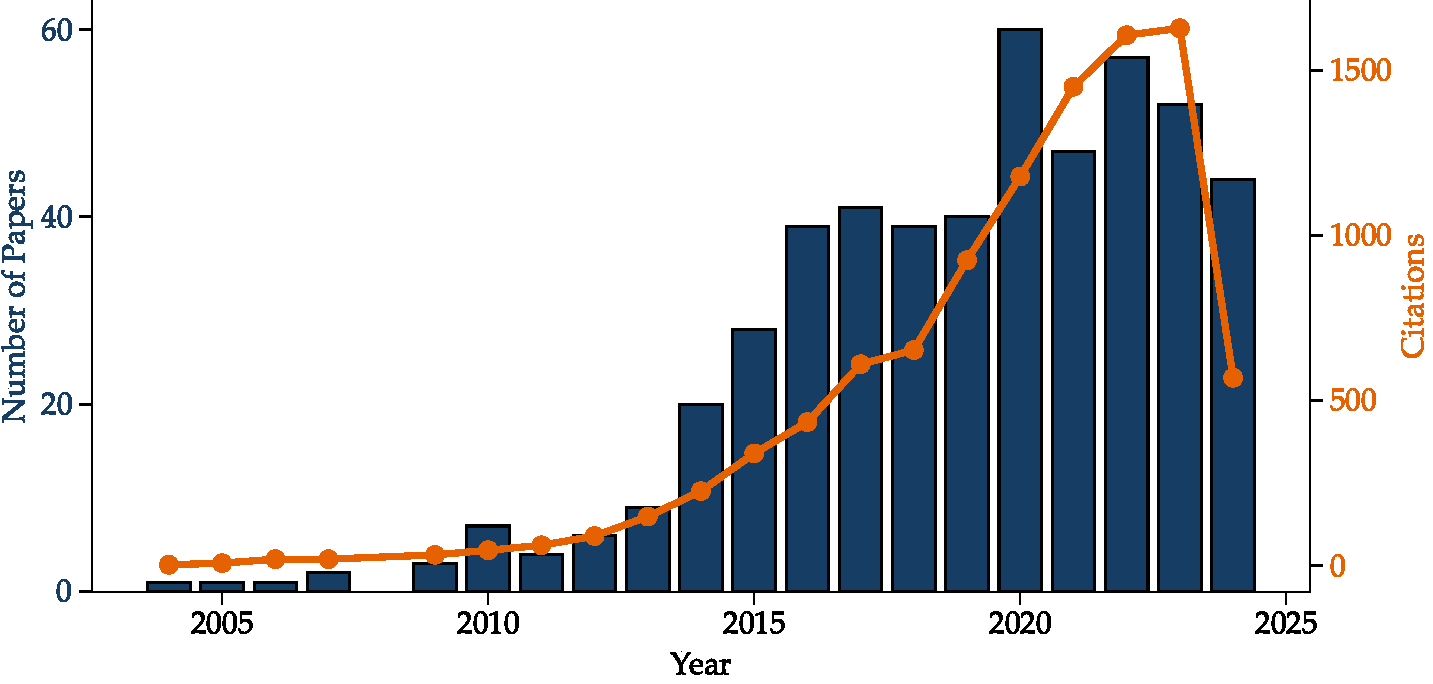
\includegraphics[width=\linewidth]{top10.pdf}
	    \caption{Published papers on hyper-reduction over the last two decades (as of 2024, \textit{source: web of science})}
\label{fig:papers}
\end{figure}



\begin{figure}[t]
	    \centering
	    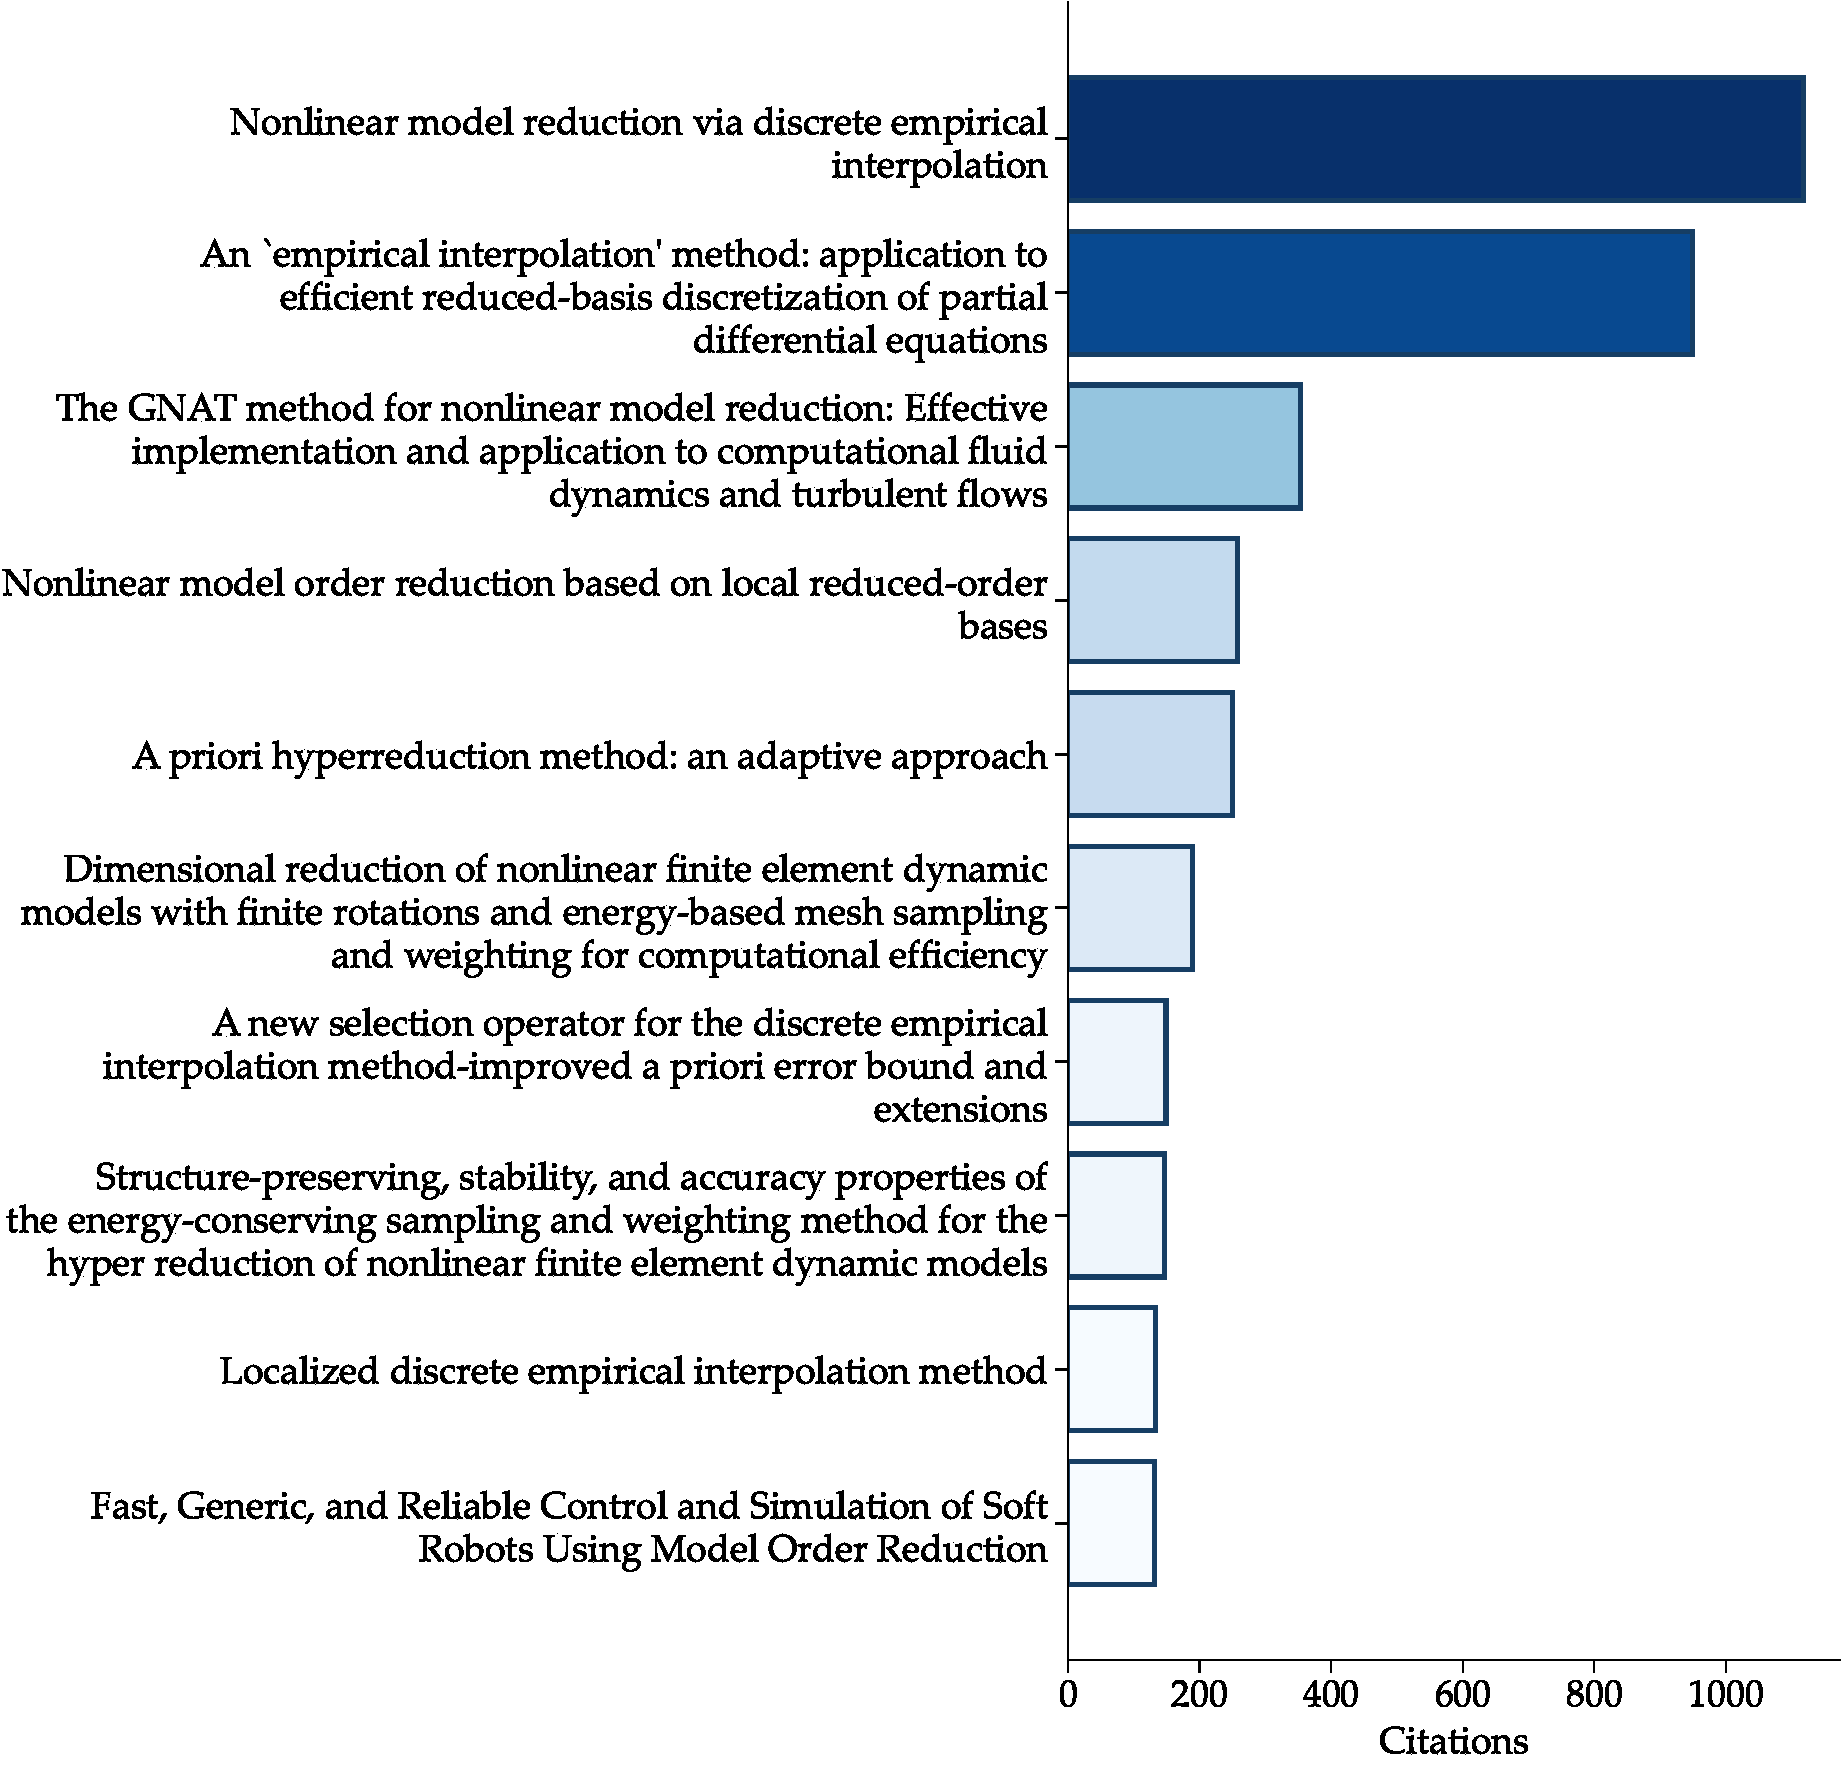
\includegraphics[width=0.8\linewidth]{papers.pdf}
	    \caption{Top 10 highly cited papers on hyper-reduction (as of 2024, \textit{source: web of science}) \cite{chaturantabut2010nonlinear,barrault2004empirical,carlberg2013gnat,amsallem2012nonlinear,ryckelynck2005priori,farhat2014dimensional,drmac2016new,farhat2015structure-preserving,peherstorfer2014localized,goury2018fast}}
\label{fig:citations}
\end{figure}

\begin{figure}[t]
    \centering
    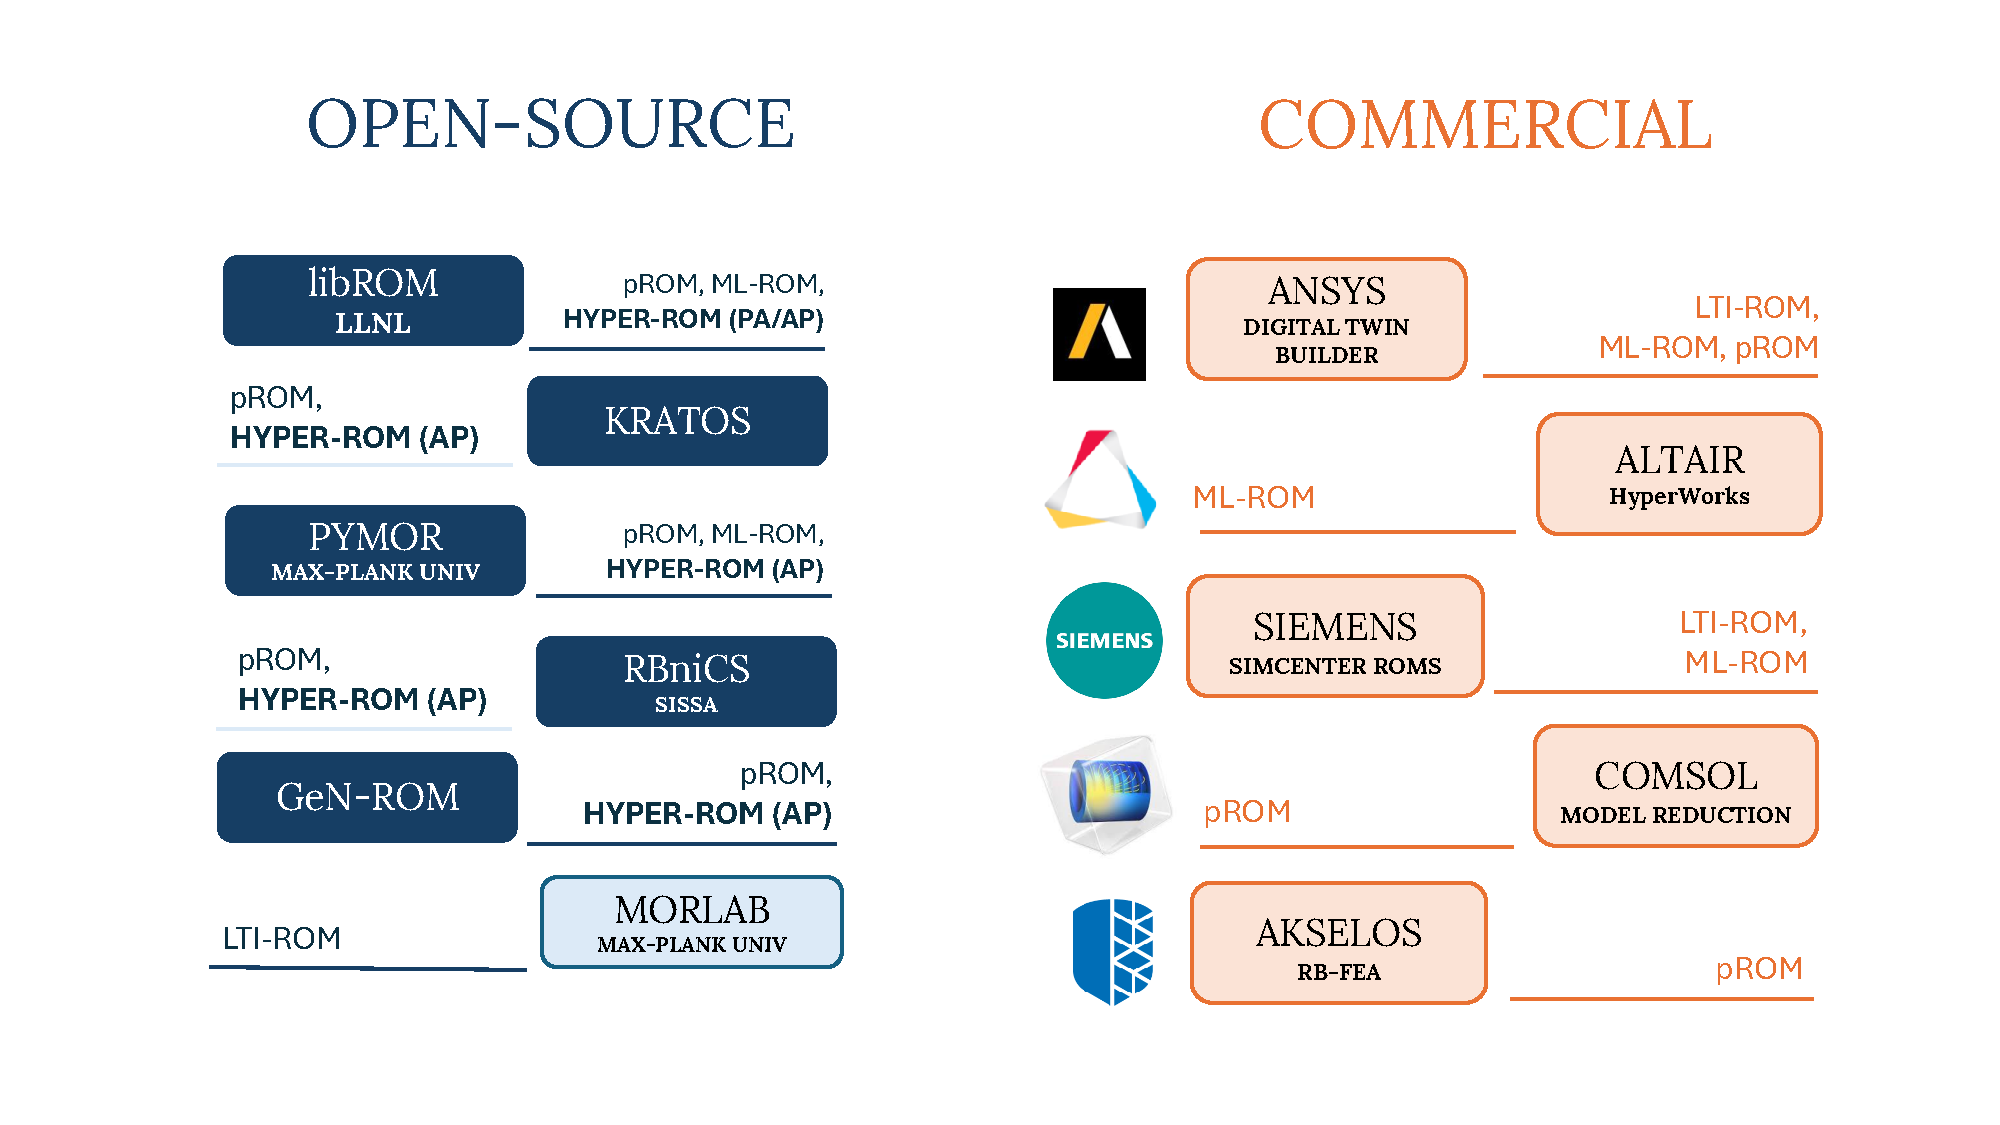
\includegraphics[width=0.9\textwidth]{software_survey5.pdf}
    \caption{Comparison of open-source and commercial software tools for reduced-order modeling (ROM) \protect\footnotemark. Open-source tools include libROM \cite{Choi2019libROM}, Kratos \cite{vicente_mataix_ferrandiz_2022_6395887}, PyMOR \cite{milk2016pymor}, RBniCS \cite{RozzaBallarinScandurraPichi2024}, and MORLAB \cite{BenW21c}. These tools support ROM methods like projection-based Reduced Order Model (pROM), Machine Learning-based ROM (ML-ROM) \cite{Drakoulas_2023,TANNOUS_2024}, Hyper-ROM (AP/PA), and Linear Time-Invariant ROM (LTI-ROM) \cite{Sikander_2017}. Dark blue boxes indicate support for Hyper-ROM, where (AP) denotes ``Approximate-then-Project,'' and (PA) denotes ``Project-then-Approximate.'' Commercial tools include ANSYS Digital Twin Builder, Altair HyperWorks, Siemens Simcenter ROMS, COMSOL Model Reduction \cite{saha2019reduced,deng2021reduced-order,Zhang_2021}, and Akselos RB-FEA \cite{Di_Nicola_2024,Sharma_2018,BRENNER_2023}, which support various ROM methods. However, none of these commercial tools support hyper-reduction.}
    \label{fig:ROM_software}
\end{figure}
\footnotetext{list not exhaustive}

The approximate-then-project methods originated with the gappy proper orthogonal decomposition (POD) method \cite{everson1995karhunen--loeve}, initially developed for image reconstruction from marred images with only a few available pixels.
In these methods, nonlinear terms are first approximated by interpolating information at a selected subset of nodes within the computational mesh, as in the image reconstruction problem, using a few empirically derived basis functions.
These approximations are then exactly projected onto the reduced subspace while formulating the ROM.
Examples include the empirical interpolation method (EIM) \cite{Hesthaven2016,barrault2004empirical}, the best points interpolation method \cite{nguyen2007best}, and the discrete empirical interpolation method (DEIM) \cite{chaturantabut2010nonlinear}—a widely used discrete version of EIM that has inspired numerous adaptations.
Variants like the missing point estimation method and the collocation method \cite{astrid2008missing,gomez2016variational} have also been developed.
Such selective evaluation of the nonlinear term at a few grid points leads to significant computational speed-ups.


Project-then-approximate methods, on the other hand, estimate the \textit{reduced-order} vectors and matrices resulting from projecting the nonlinearities of the high-fidelity model (HFM) onto the latent space.
These methods generate a reduced mesh by selecting a subset of elements or entities from the full computational mesh with an aim to directly calculate the projected nonlinearity, closely approximating the true projected nonlinearity of the complete mesh.
These methods aim for more accurate and robust pROM approximations compared to the approximate-then-project approach.
They can be viewed as generalized quadrature rules, where quadrature points and weights are learned—leading to effective mesh sampling \cite{chapman2016accelerated}.
Examples include the energy-conserving sampling and weighting method \cite{farhat2015structure-preserving,tezaur2022robust,maierhofer2022model,farhat2014dimensional}, the empirical cubature method (ECM) \cite{hernandez2014high,bravo2024subspace,hernandez2020multiscale,hernandez2024cecm}, and the linear program-based empirical quadrature method (EQP) \cite{yano2019lp}.
Henceforth, we shall refer to pROMs that implement hyper-reduction strategies as Hyper-ROMs.



Over the past two decades, hyper-reduction techniques have gained significant traction in the scientific community, as illustrated by the increase in published papers on the topic as seen in \cref{fig:papers}.
The number of publications reached its peak around 2021, while citations have continued to grow steadily, highlighting the sustained impact and active engagement of researchers in the field.
Among the most highly cited papers, methods such as (D)EIM  and the GNAT \cite{carlberg2013gnat,jiang2019implementation} stand out as pivotal contributions (\cref{fig:citations}).

Hyper-ROMs find extensive application in domains such as reservoir simulations \cite{Jansen_2016,ghasemi2016localized,yoon2016hyper-reduced-order,Tan_2018,Jiang_2019_gnat,ghommem2016complexity,he2014reduced}, nuclear engineering \cite{german2019application,tano2021evaluation}, mechanical and aerospace engineering \cite{tiso2013discrete,antil2014application,farhat2014dimensional,hernandez2017dimensional,farhat2021_5_bookchapter,farhat2015structure-preserving,grimberg2021mesh}. %
Notably, they are capable of playing a critical role in the development and deployment of digital twin technology \cite{sharma2022digital,botin-sanabria2022digital,liu2021review,kapteyn2020toward}.
Digital twins serve as virtual counterparts of physical systems, enabling real-time monitoring, analysis, and decision-making.
These functionalities depend on the rapid and precise simulations, which can be provided by such Hyper-ROMs,  facilitating the prediction of system responses across various scenarios.


The current landscape of software tools supporting hyper-reduction, depicted in \cref{fig:ROM_software}, reveals a distinct divide between open-source and commercial offerings.
Open-source software like libROM \cite{Choi2019libROM}, PyMOR \cite{milk2016pymor}, and MORLAB \cite{BenW21c} provide comprehensive capabilities for hyper-reduction, which serve as important resources for academic researchers.
On the other hand, commercial tools such as ANSYS \cite{asgari2014application,pliuhin2023implementation}, Siemens Simcenter ROMS \cite{Siemens2021simcenterd}, and Altair HyperWorks \cite{lindqvist2022method} have yet to incorporate hyper-reduction methodologies.
This gap presents a missed opportunity for commercial platforms, as integrating hyper-reduction could significantly enhance computational efficiency, particularly in fields where real-time decision-making and large-scale simulations are crucial.
The lack of hyper-reduction capabilities in commercial software, as illustrated in \cref{fig:ROM_software}, is primarily due to the intrusive nature of these techniques.
Implementing hyper-reduction requires extensive modifications to existing codebases and databases within well-established computational pipelines.
Open-source tools tend to have more flexibility to integrate such methods, but commercial platforms prioritize stability and broad applicability.
This focus makes it challenging to adopt hyper-reduction without causing significant disruptions.
Nonetheless, this situation underscores both the difficulty and the substantial potential benefits for commercial vendors to enhance their software by incorporating hyper-reduction methods.


Now, in addition to hyper-reduction, other strategies exist for addressing nonlinearities in models.
For polynomial nonlinearities \cite{ghattas2021learning}, the nonlinear terms can be exactly reduced on the latent linear subspace without hyper-reduction.
In Ref.~\cite{gu2011qlmor} it was shown that nonlinear dynamical systems could be transformed into a quadratic-bilinear form using auxiliary variables, with the number of variables increasing linearly with the system's nonlinear functions.
This method, applicable to various nonlinearities in engineering systems, was further extended for model reduction in systems governed by PDEs in \cite{benner2015two-sided,kramer2019nonlinear,kramer2021balanced}.
These works highlight lifting of nonlinearities to quadratic form as an effective alternative to hyper-reduction.


Furthermore, beyond the POD-based linear reduction methods, nonlinear model reduction techniques \cite{Amsallem_2012,hahn2002improved,dong2003piecewise,carlberg2013gnat,carlberg2015preserving,chaturantabut2012state,rowley2017model,daronch2012nonlinear} have also been developed to deal with nonlinear systems.
Unlike POD-ROMs, which assume that the solution lies within a linear subspace, nonlinear model reduction \cite{Touz__2021,shaw1991non-linear,Chen_1996,daniel2022physics,borggaard2016goal} assumes that the solution resides on a manifold—a curved structure—in the state space (e.g., displacement and velocity for second-order systems) \cite{glad2018control,trentelman2002control}.
These manifolds are defined as nonlinear functions of the state variables, and their structure is typically inferred using physics-based insights.
For instance, the authors in \cite{Rutzmoser_2017,jain2017quadratic} presented strategies to derive quadratic manifolds for the reduced-order modeling of geometrically nonlinear structural dynamic systems.
These quadratic manifolds were demonstrated to effectively capture the physical behaviors of such systems.
In contrast, \cite{kim2022fast} adopted a non-intrusive approach by employing a deep neural network to approximate the solution manifold, thereby avoiding the need to alter the original system equations or directly derive the manifold analytically.


For systems characterized by both slow and fast dynamics, invariant manifolds \cite{gorban2004constructive,cabre2005parameterization,shaw1991non-linear,simo1989analytical,guckenheimer2004fast,ascher1994stabilization} serve as optimal spaces for model reduction.
Because these manifolds are invariant under the action of the dynamical system, any trajectory starting on one remains there indefinitely.
This property ensures that the trajectories captured by the reduced-order model (ROM) are consistent with those of the full system.
Additionally, the curvature of these manifolds embodies nonresonant couplings \cite{shami2022nonlinear,Touz__2021,Lacarbonara_2003}, enabling the representation of coupled modes without the need for additional vector bases or complex sorting methods.
Essentially, utilizing invariant manifolds transforms model reduction into a geometric problem in phase space \cite{nolte2010tangled,cenedese2022data}, offering a powerful tool for handling nonlinearities in large-scale systems.

While these methods show promise, and in some cases, outperform hyper-reduction techniques in efficiency, hyper-reduction has seen broader application across multiple domains, yielding reliable results.
Given the growing interest in data-driven reduced-order modeling for nonlinear systems in recent years, it is essential to develop a thorough understanding of this powerful tool.
While some articles provide brief overviews of the algorithms \cite{kim2021improved}, comprehensive discussions are often outside their scope.
A few excellent texts published recently offer in-depth insights into data-driven surrogate and reduced-order models in general \cite{benner_2021,brunton2019data-driven,ghattas2021learning,fu2018pod}, few focus specifically on hyper-reduction methods \cite{Nguyen2024}.
Furthermore, the principles and algorithms of hyper-reduction are often deeply mathematical in nature, presenting a steep learning curve for researchers new to the field.


In this tutorial review, we aim to bridge this gap by adopting a more intuitive approach whenever possible.
We focus on simpler nonlinear problems to emphasize easy interpretability and make the concepts more accessible to beginners.
To facilitate practical understanding, we also share an accompanying GitHub code repository that provides hands-on examples and implementations of the discussed methods.


The paper is organized as follows: First, %
we present a detailed overview of projection-based ROMs, focusing on POD.
This includes the associated minimization problem, methods for determining the reduced subspace dimension, and the connection between POD and singular value decomposition.
In Section 3, we present a one-dimensional heat conduction problem as a representative case to illustrate model reduction both without and with various hyper-reduction techniques.
We selected this problem for its conceptual clarity and ease of understanding, while recognizing that hyper-reduction methods have already been established as effective in large-scale, complex settings.
Our choice of this problem facilitates a more tutorial-oriented demonstration.
Finally, in Section 4, we discuss various hyper-reduction techniques, starting with approximate-then-project strategies such as Gappy-POD, the Discrete Empirical Interpolation Method (DEIM), S-OPT, and Gauss-Newton with Approximated Tensors (GNAT), as well as project-then-approximate strategies like Energy Conserving Sampling and weighing, and the Empirical Cubature Method, and compare these methods using the toy problem.
We also briefly explore deep-learning-based hyper-reduction approaches, which utilize neural networks.
We conclude by discussing future directions and potential applications of these methodologies in advancing computational efficiency across various engineering disciplines.
This tutorial review emphasizes quantitative understanding in a manner suitable for back-of-the-envelope calculations, with an aim to provide reusable insights.
\section{Background and preliminaries}


Projection-based reduced-order modeling (ROM) problems can generally be categorized into two main types \cite{benner_2021}.
The first category of problems deals with large-scale models formulated based on a system-theoretic approach.
These models are characterized by a large set of Ordinary Differential Equations (ODEs) or Differential-Algebraic Equations (DAEs), e.g., linear-time-invariant (LTI) systems, where the dynamics is represented using state variables.
The state variables evolve with time, being driven by external excitation, and are partially captured at the output phase based on the quantities of interest.
The ROMs preserve the original structure of these large-scale models and use a reduced state while closely matching the input-output relation of the actual system.
Furthermore, the model reduction algorithms used for these problems are not strictly data-driven, but are often performed based on the characteristics of the full-order model without relying upon simulation data.
In essence, these algorithms determine a reduced subspace for projecting the full-order models which results in eliminating the state variables that are poorly coupled with the input-forcing and barely contribute to the observed outputs.
Examples of such systems include Balanced truncation \cite{moore2003principal}, moment matching methods \cite{benner2015survey,rowley2005model}, etc.
While effective for large-scale \textit{linear systems} (e.g., Linear Time Invariant --LTI), their applicability to multi-input multi-output nonlinear systems is limited.



The second category of problems centers on the accelerated numerical solution of Partial Differential Equations (PDEs), which are inherently infinite-dimensional.
As depicted in \cref{fig:ROM_FOM_schematic}, the numerical solution of PDEs typically involves a three-stage process.
First, the infinite-dimensional domain is discretized into a finite-dimensional space.
This discretization may take the form of nodal values (finite element method), point values (finite difference method), or cell averages (finite volume method), among others, depending on the chosen numerical method.
To ensure sufficiently fidelity, the dimensionality of this finite representation is often chosen very large (e.g., using a fine spatial mesh), resulting in a transformation of the PDEs into a high-dimensional system of algebraic, differential, or differential-algebraic equations.
Next, standard numerical techniques are applied to solve these equations, a process that is computationally demanding due to the large dimensionality.
Finally, once a solution is obtained, it is mapped back from the finite-dimensional space encoded space to the original infinite-dimensional space using polynomial interpolation or Galerkin projections.


\emph{Reduced-order models} further simplify the computational burden of these high-fidelity, large-scale systems by \emph{compressing} the finite-dimensional space into a much smaller latent space.
The large-scale equations are then projected onto this latent space to formulate a reduced system.
After solving these reduced equations, the solution is first interpolated back to the finite, high-dimensional space, and then further mapped to the infinite-dimensional space, as in the standard process described above.
The latent space is derived directly from the high-fidelity data of the large-scale system and is typically represented  by either a low-dimensional nonlinear manifold or a low-dimensional linear subspace.
This paper focuses on the latter --linear subspace reduced order models (LS-ROMs)-- while providing a brief complementary discussion on nonlinear manifold reduced order models (NM-ROM) towards the end.


The subspace for LS-ROMs is typically obtained by applying proper orthogonal decomposition (POD) or singular value decomposition (SVD) onto a small volume of the high-fidelity (training) data.
POD hierarchically captures the dominant correlations within the data using orthonormal basis vectors, also known as proper orthogonal modes, and thereby captures the few dominant low-rank characteristics of the high-fidelity \textit{model} itself.
The process of deriving a projection based LS-ROM is described in detail in the following subsections.

\begin{figure}[t]
\centering
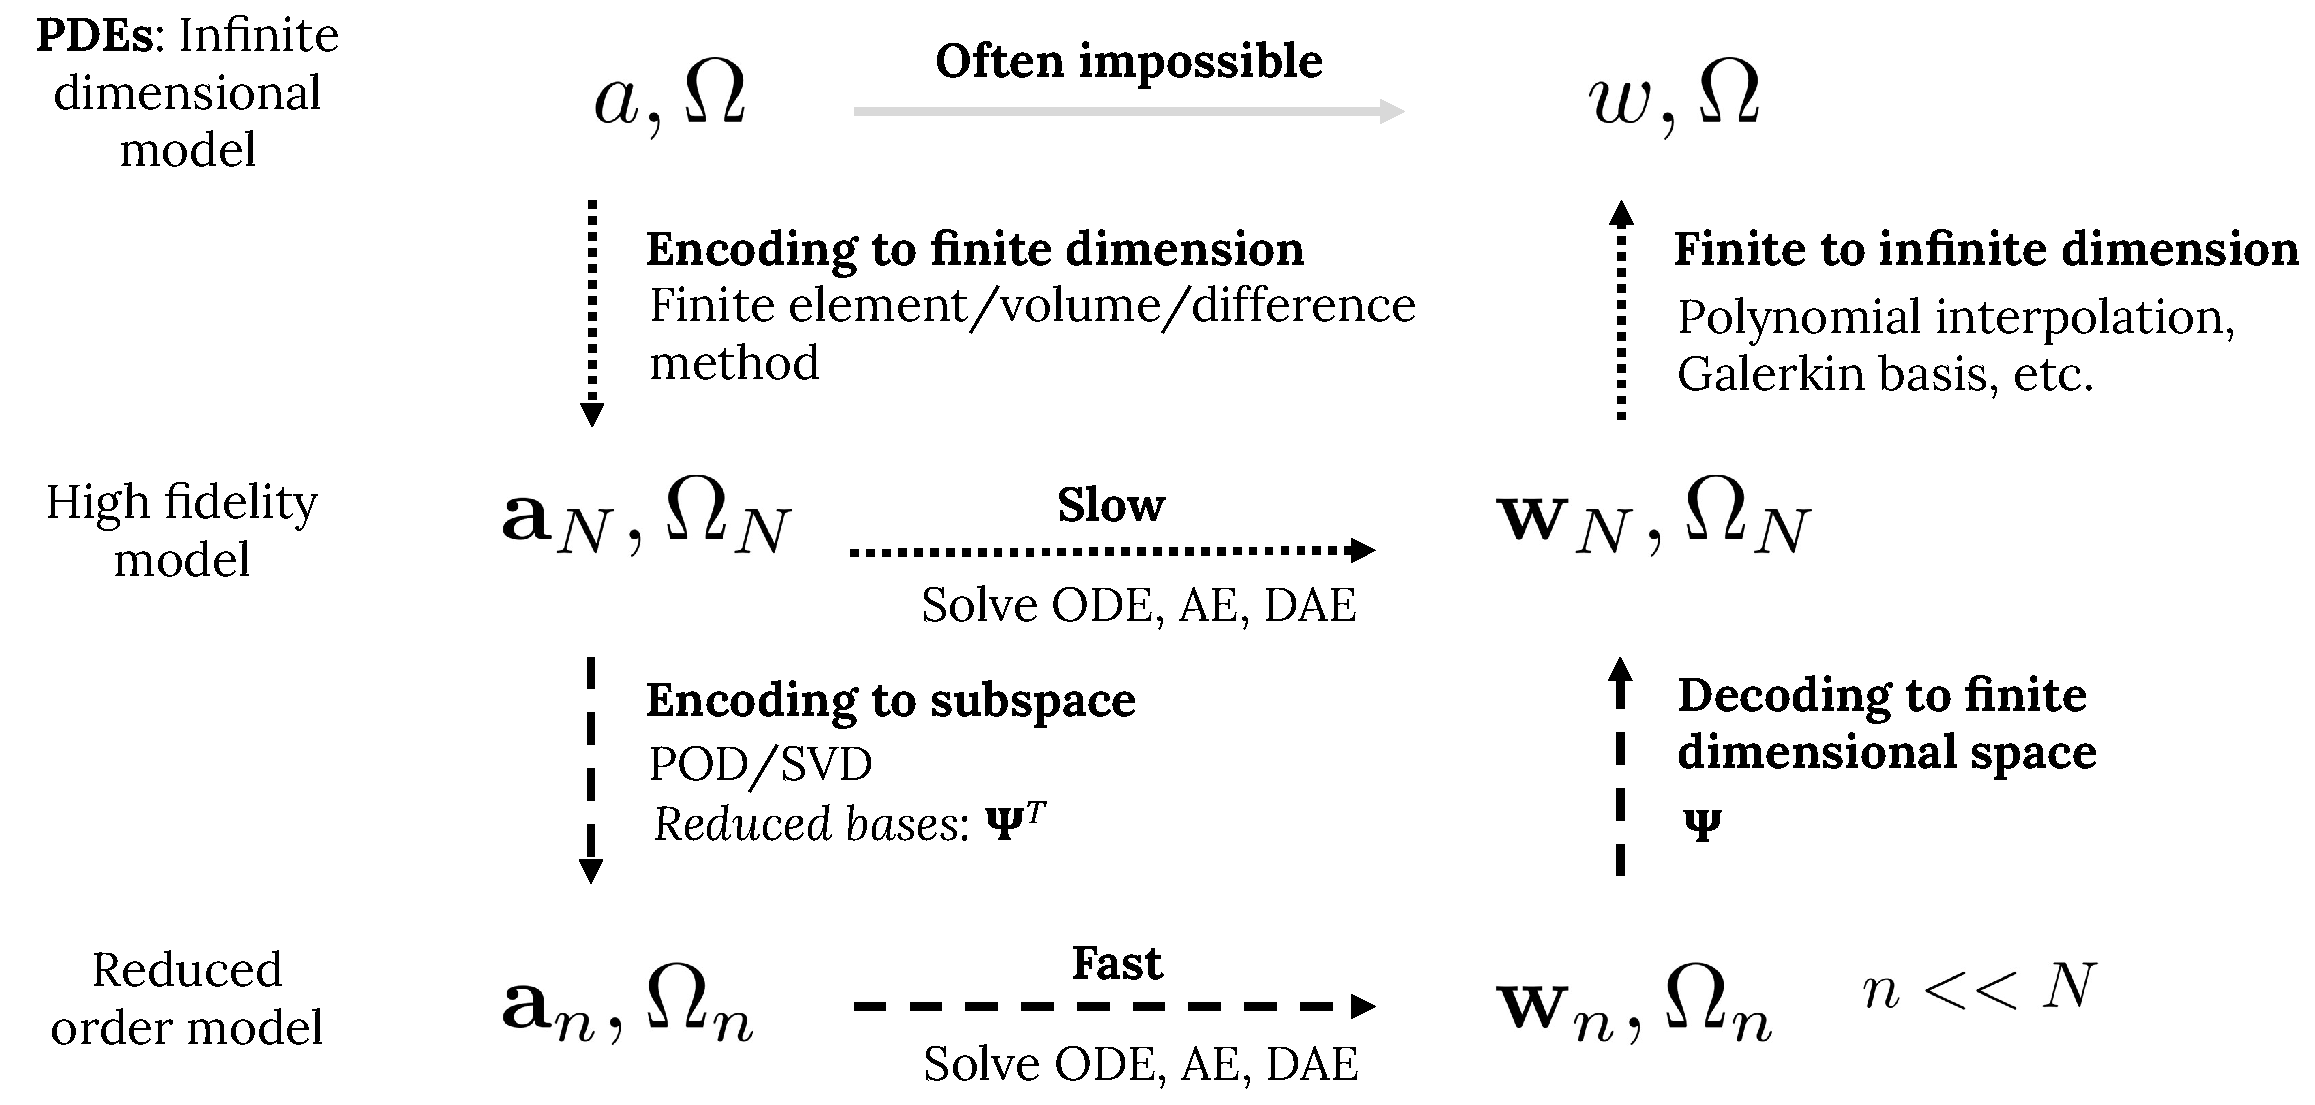
\includegraphics[width=0.8\textwidth]{schematic.pdf}
\caption{Numerical solution of PDEs. High-fidelity models and reduced order models. Here $a$ represents an input to the system; $\Omega$ is the problem domain in the infinite dimensional space, $w$ is the infinite-dimensional solution to the PDE; $\vec{a}_N$, $\vec{w}_N$ and $\Omega_N$ are the high-dimensional finite approximation, and $\vec{a}_n$, $\vec{w}_n$ and $\Omega_n$ are the reduced representation of  $\vec{a}$, $\Omega$, and $\vec{w}$, respectively.}
\label{fig:ROM_FOM_schematic}
\end{figure}

\subsection{The high-fidelity model}

Let us consider a parametric, time-dependent, semi-discrete (discretized in space only), $N$-dimensional ($N$ prohibitively large) high-fidelity model defined over domain $\Omega_N$, which is of the form \cite{benner_2021}
\begin{equation}
\left\{
\begin{array}{l}
\mat{M}(\boldsymbol{\mu})\dot{\vec{w}}(\vec{x},t; \boldsymbol{\mu}) + \vec{f}(\vec{w}(\vec{x},t; \boldsymbol{\mu}); \boldsymbol{\mu}) = \vec{g}(\vec{x},t; \boldsymbol{\mu}),\\
\vec{w}(\vec{x},0; \boldsymbol{\mu}) = \vec{w}^0(\vec{x};\boldsymbol{\mu}),
\end{array}
\right.
\label{eq:gov_eq}
\end{equation}
where $\vec{x}\in\Omega_N$; $t$ is time; $\boldsymbol{\mu}$ is a parameter vector in bounded space $P \subset \mathcal{R}^p$; $M(\boldsymbol{\mu}) \in \mathcal{R}^{N \times N}$ is the symmetric, positive definite mass matrix; $\vec{w}(\vec{x},t; \boldsymbol{\mu}) \in \mathcal{R}^{N}$ is the time-dependent state solution vector; $\vec{w}^0(\vec{x};\boldsymbol{\mu})$ is the initial condition; $\vec{f}(\vec{w}, t; \boldsymbol{\mu}) \in \mathcal{R}^{N}$ is the non-linear internal force vector; $\vec{g}(\vec{x},t; \boldsymbol{\mu}) \in \mathcal{R}^{N}$ is the time-dependent external force vector.

As shown in \cref{fig:ROM_FOM_schematic}, these high-fidelity models are obtained from the governing partial differential equations by employing techniques like finite difference/element/volume methods.
Constructing a projection-based reduced-order model (ROM) for \cref{eq:gov_eq} involves three stages: (a) generating a small dataset of high-fidelity training data by solving \cref{eq:gov_eq}, (b) determining a reduced subspace from this data using a dimension reduction method like proper orthogonal decomposition (POD) \cite{holmes1996turbulence}, and (c) projecting the high-fidelity model onto the reduced subspace to obtain a ROM \cite{benner2015survey}.

In the following two sections we discuss stages (b) and (c) assuming that a small volume of high-fidelity training data has been generated by solving \cref{eq:gov_eq}.
We present a brief description of POD first followed by the derivation of the ROM.























































\subsection{Proper orthogonal decomposition (POD)}
Proper Orthogonal Decomposition (POD), also known as Principal Component Analysis (PCA) or Karhunen-Lo\`eve Decomposition (KLD), reduces dimensionality of data by capturing dominant correlated patterns with minimal information loss \cite{chatterjee2000introductiona,holmes1996turbulence}. 
The goal is to find a reduced set of orthonormal basis functions that represent the dataset optimally.

More formally, POD seeks an optimal basis $U(x)$ by minimizing the error in the time-averaged projection of a spatio-temporal field $w(x,t)$:
\begin{equation}
 \underset{ U \in L^2(\Omega)}{\operatorname{min}} \Big \langle \| w(x,t) - ( w(x,t), U(x) ) U(x) \|^{2} \Big \rangle   
\end{equation}
subject to $\| U(x) \| = 1$. This can be reformulated as a maximization problem, leading to the eigenvalue problem:
\begin{equation}
\mathfrak{R} U = \lambda U, \quad \mathfrak{R} U = \langle (w, U)w \rangle,
\end{equation}
where $\mathfrak{R}$ is the covariance operator, and the eigenfunctions $U$ are termed proper orthogonal modes (POMs). The eigenvalues $\lambda$ indicate the variance captured by each mode. POMs are ranked by decreasing eigenvalue magnitude.

The reduced subspace is constructed by selecting the first $n$ POMs such that the cumulative variance fraction $r_k$ exceeds a threshold $\alpha$, often set close to 1. We define $r_k$ as:
\begin{equation}
r_k = \frac{\sum_{i=1}^k \lambda_i}{\sum_{i=1}^N \lambda_i}
\label{eq:mode_sel}
\end{equation}
The reconstruction error after projecting onto a $k$-dimensional subspace with $r_k \geq \alpha$ is given by \cite{bhattacharyya2020energy}:
\begin{equation}
\epsilon_{\text{POD}} = \sqrt{\sum_{i=k+1}^N \lambda_i}
\end{equation}


In practical applications, POD is commonly computed on the discrete data snapshots. 
Assuming a spatial discretization $N$, and temporal discretization $N_t$, we define the snapshot matrix, \(\mat{W}\in\mathsf{R}^{N\times N_t}\) as:
\begin{equation}
	\mat{W}=\left[\begin{array}{cccc}
	\mathbf{w}_{1} - \mathbf{w}^{ref} & \mathbf{w}_{2} - \mathbf{w}^{ref}& \cdots & \mathbf{w}_{N_t} - \mathbf{w}^{ref}\\
	\end{array}\right]
\label{eq:data_W}
\end{equation}
where the columns of $\mat{W}$ are the zero-mean solution vectors collected at specific time instances or parameter values, and $\mathbf{w}^{ref}\in\mathcal{R}^{N}$ denotes a reference, often taken to be the mean vector of the solution snapshots. 
The covariance \textit{matrix} is then given by:
\begin{equation}
\mat{R} = \frac{1}{N_t}\mat{W}\mat{W}^\top
\label{eq:cor_mat}
\end{equation}
Often times, directly solving the eigenvalue problem \(\mat{R}\vec{U} = \lambda\vec{U}\) is computationally expensive for large \(N\). 
To address this, the \textit{method of snapshots} was introduced \cite{sirovich1987low-dimensional}, which reduces the problem to a smaller eigenvalue problem of size \(N_t \times N_t\) and solve the reduced eigenvalue problem to calculate the POMs $\vec{U}$ in the following manner:
\begin{equation}
\frac{1}{N_t}\mat{W}^\top\mat{W}\vec{q} = \lambda\vec{q}, \quad \mathbb{U} = \mat{W}\vec{q}
\end{equation}


It can be shown that POD of of the snapshot matrix \(\mat{W}\)  is closely related to its Singular Value Decomposition (SVD):
\begin{equation}
\mat{W} = \underline{\mathbb{U}}\mat{\Sigma}\underline{\mathbb{V}}^\top
\label{eq:svd}
\end{equation}
where $\underline{\mathbb{U}}\in\mathcal{R}^{N \times N}$ and $\underline{\mathbb{V}}\in\mathcal{R}^{N_t \times N_t}$ contain orthonormal left and right singular vectors, respectively, with $\underline{\mathbb{U}}^\top\underline{\mathbb{U}} = \mat{I}_N$ and $\underline{\mathbb{V}}^\top\underline{\mathbb{V}} = \mat{I}_{N_t}$. The diagonal matrix $\mat{\Sigma}\in\mathcal{R}^{N \times N_t}$ contains non-negative singular values $\sigma_i$ in descending order. 
Substituting \eqref{eq:svd} into \eqref{eq:cor_mat} yields:
\begin{equation}
\mat{R} = \frac{1}{N_t} \underline{\mathbb{U}} \mat{\Sigma} \mat{\Sigma}^\top \underline{\mathbb{U}}^\top = \underline{\mathbb{U}}\mat{\Lambda}\underline{\mathbb{U}}^\top
\label{eq:pod-svd}
\end{equation}
where $\mat{\Lambda} = \dfrac{1}{N_t}\mat{\Sigma}\mat{\Sigma}^\top$.
\cref{eq:pod-svd} shows that the principal components or the eigenvectors obtained from the POD of $W$ are essentially same as the left singular vectors of the SVD of $W$, with eigenvalues linked to squared singular values. 
The elements of $\mat{\Lambda}$ satisfy:
\begin{equation}
\frac{\sigma_i^2}{N_t} = \lambda_{\text{POD}_i}
\label{eq:SVD_POD}
\end{equation}
Hence, SVD is directly applied to $\mat{W}$ for reduced subspace construction.




\subsection{Reduced order model}
\label{sec:ROM}
In a discrete setting, the subspace for the ROM  is spanned by a truncated set of basis vectors contained a matrix $\widetilde{\mathbb{U}}\in\mathcal{R}^{N\times n}$:

\begin{equation}
\widetilde{\mathbb{U}} = \mathbb{U}[:,1:n]
\label{eq:U_tilde}
\end{equation}

where $n$ is the number of vectors retained after truncation.
Then the solution of \cref{eq:gov_eq} is approximated as
\begin{equation}
\vec{w}_N(\vec{x},t; \boldsymbol{\mu}) \approx \widetilde{\vec{w}}_N(\vec{x},t; \boldsymbol{\mu}) = \vec{w}^{ref}_N+\widetilde{\mathbb{U}}  \vec{w}_n(\vec{x},t; \boldsymbol{\mu}),
\label{eq:w_ned_gal}
\end{equation}
where $\vec{w}_n$ are the reduced coordinates of the basis vectors in $\widetilde{\mathbb{U}}$.
Formally $\widetilde{\mathbb{U}}$ is called the left reduced order basis or left ROB.
Substituting $\widetilde{\vec{w}}_N$ in \cref{eq:gov_eq}, we obtain the following residual:
\begin{equation}
\vec{r}_{N}(\vec{w}_n;\boldsymbol{\mu}) = \mat{M}(\boldsymbol{\mu})\widetilde{\mathbb{U}}\dot{\vec{w}}_n(\vec{x},t; \boldsymbol{\mu}) + \vec{f}_N(\vec{w}^{ref}_N+\widetilde{\mathbb{U}}\vec{w}_n(\vec{x},t; \boldsymbol{\mu}); \boldsymbol{\mu}) - \vec{g}_N(\vec{x},t; \boldsymbol{\mu})
\label{eq:residual_gov_eq_gal}
\end{equation}


A direct solution to $\vec{r}_N=0$ is not possible since the system is over-determinate ($N$ equations but $n$ unknowns).
Typically, we constrain the residual by enforcing it to be orthogonal to a test subspace spanned by another set of basis vectors ${\mathbb{W}}\in\mathcal{R}^{N\times n}$, termed as the right reduced order basis or right ROB, such that

\begin{equation}
\mathbb{W}^\top \left[ \mat{M}(\boldsymbol{\mu}) \widetilde{\mathbb{U}} \dot{\vec{w}}_n + \vec{f}_N(\vec{w}^{ref}_N+\widetilde{\mathbb{U}} \vec{w}_n; \boldsymbol{\mu}) - \vec{g}_N \right] = 0.
\label{eq:PG_projection}
\end{equation}

This yields a $n$-dimensional solvable system of equations.
Defining the reduced-order matrices and vectors as
\begin{equation}
\mat{M}_{n}(\boldsymbol{\mu}) = \mathbb{W}^\top \mat{M}_{N}(\boldsymbol{\mu}) \widetilde{\mathbb{U}},
\end{equation}
\begin{equation}
\vec{f}_n(\vec{w}; \boldsymbol{\mu}) = \mathbb{W}^\top \vec{f}_N(\vec{w}^{ref}_N+\widetilde{\mathbb{U}} \vec{w}_n; \boldsymbol{\mu}),
\end{equation}
\begin{equation}
\vec{g}_n = \mathbb{W}^\top \vec{g}_N,
\end{equation}

and assuming that $(\mathbb{W}^\top \widetilde{\mathbb{U}})$ is invertible, we write this {descriptive form} of the \textit{Petrov-Galerkin} reduced-order model as \cite{stanford_cme345}
\begin{equation}
\left\{
\begin{array}{l}
\mat{M}_n(\boldsymbol{\mu}) \dot{\vec{w}}_n + \vec{f}_n(\vec{w}_n; \boldsymbol{\mu}) = \vec{g}_n,\\
\vec{w}_n(\vec{x},0, \boldsymbol{\mu}) = (\mathbb{W}^\top \widetilde{\mathbb{U}})^{-1}\mathbb{W}^\top (\vec{w}_N^0(\boldsymbol{\mu})-\vec{w}^{ref}_N)
\end{array}
\right.
\label{eq:ROM_eq}
\end{equation}


The $n-$dimensional ROM in \cref{eq:ROM_eq} is solved at a much lower computational cost, and the approximate full order solution is reconstructed using \cref{eq:w_ned_gal}.
Note that, \cref{eq:ROM_eq} can also be obtained using the more commonly employed \textit{Galerkin Projection}, in which  $\mathbb{W}=\widetilde{\mathbb{U}}$ and  $(\mathbb{W}^\top \widetilde{\mathbb{U}})=\mat{I}_{n}$.















\section{Model reduction for 1D parametric heat conduction}
\label{sec:ROM_example}

In this section, we discuss the model reduction of a 1D linear and a 1D nonlinear heat conduction problem, characterized by parametric elliptic PDEs, and demonstrate the efficacy of projection-based reduced order modeling.
We briefly describe the finite element formulation of the governing PDE to obtain the high-fidelity model, and subsequently derive the corresponding reduced order model following the steps delineated in the previous sections.
Though here our discuss centers around a finite element model, as discussed earlier, any other encoding strategy such as finite difference or finite volume method can be employed as well \cite{farhat2020computational}.


The governing equation for steady state heat conduction over a 1D domain $\Omega = [0,0.5]$ is given by
\begin{equation}
-\nabla \cdot (k \nabla T) = q \quad \text{in} \quad \Omega,
\label{eq:heat_pde}
\end{equation}
where $k$ ({\unit{\watt\per\meter\per\kelvin}}) is the thermal conductivity, which can either be a linear function of the parameter vector $\boldsymbol{\mu}$ or a nonlinear function of both $\boldsymbol{\mu}$ and the temperature field $T$ ({\unit{\kelvin}}), and \( q \) (\unit{\watt\per\meter}) is the internal heat generation per unit length.
While this section covers both cases—linear and nonlinear \( k \)—the following formulations assume $k$ is nonlinear.
Equivalent formulations apply when \( k \) is linear.


Furthermore, denoting \( g \)  as the heat flux on the boundary, the Neumann and the Dirichlet boundary conditions for both the linear and the nonlinear problems are defined as
\begin{equation}
   \left. g\right|_{x = 0} = 0\, \unit{W} \quad \text{and} \quad \left.T\right|_{x = 0.5} = 573.15 \, \text{K} 
\end{equation}





To obtain a finite element model, we begin by deriving the weak form of \cref{eq:heat_pde} \cite{nreddy2018introduction,hughes2012finite}.
This process requires defining the trial space \( \mathcal{U} \) and the test space \( \mathcal{V} \).
The trial space \( \mathcal{U} \) encompasses admissible temperature functions \( T \) that comply with essential boundary conditions, while the test space \( \mathcal{V} \) includes test functions \( v \) that vanish on these boundaries.
The weak form is derived by multiplying the governing PDE by a test function \( v \in \mathcal{V} \) and integrating over the domain \( \Omega \):

\begin{equation}
\int_{\Omega} k(T;\boldsymbol\mu)\nabla T \cdot \nabla v \, d\Omega  = \int_{\Omega} q v \, d\Omega 
\label{eq:weak_pde}
\end{equation}


We write the approximate solution of \cref{eq:weak_pde} \( \widehat{T}(x) \in \mathcal{U} \), in terms of finite element basis functions also known as the shape function as

\begin{equation}
\widehat{T}(x) \approx \sum_{i=1}^{N} T_i \phi_i(x),
\label{eq:FE_shape}
\end{equation}

where \( \phi_i(x) \in \mathcal{U} \) are the 1-D linear Lagrange basis functions  defined over \( \Omega \), and \( T_i \) are the associated coefficients.
Since the shape functions \( \phi_i \) belong to the trial space \( \mathcal{U} \), they satisfy the essential boundary conditions, ensuring that the approximate solution \( T(x) \) is also admissible.

We select the test functions \( v \) to be identical to \( \phi_i \) (Galerkin projection), which yields a system of nonlinear algebraic equations (or linear, if \( k \) is linear):

\begin{equation}
\mat{K}_N(\vec{T}_N;\boldsymbol\mu) \vec{T}_N = \vec{f}_N
\label{eq:HC_HDM}
\end{equation}






where we write 
\begin{equation}
\mat{K}_N(\mathbf{T}_N; \boldsymbol\mu) = \sum_{e=1}^{n_{\text{cell}}} \mat{Q}_e^\top \mat{K}^e (\mat{Q}_e\mathbf{T}_N; \boldsymbol\mu) \mat{Q}_e,
\label{eq:elemental_contrib_K}
\end{equation}
\begin{equation}
\mathbf{f}_N = \sum_{e=1}^{n_{\text{cell}}} \mat{Q}_e^\top \vec{f}^e_{d_e}(\boldsymbol\mu),
\label{eq:elemental_contrib_f}
\end{equation}

\begin{figure}[t]
    \centering
    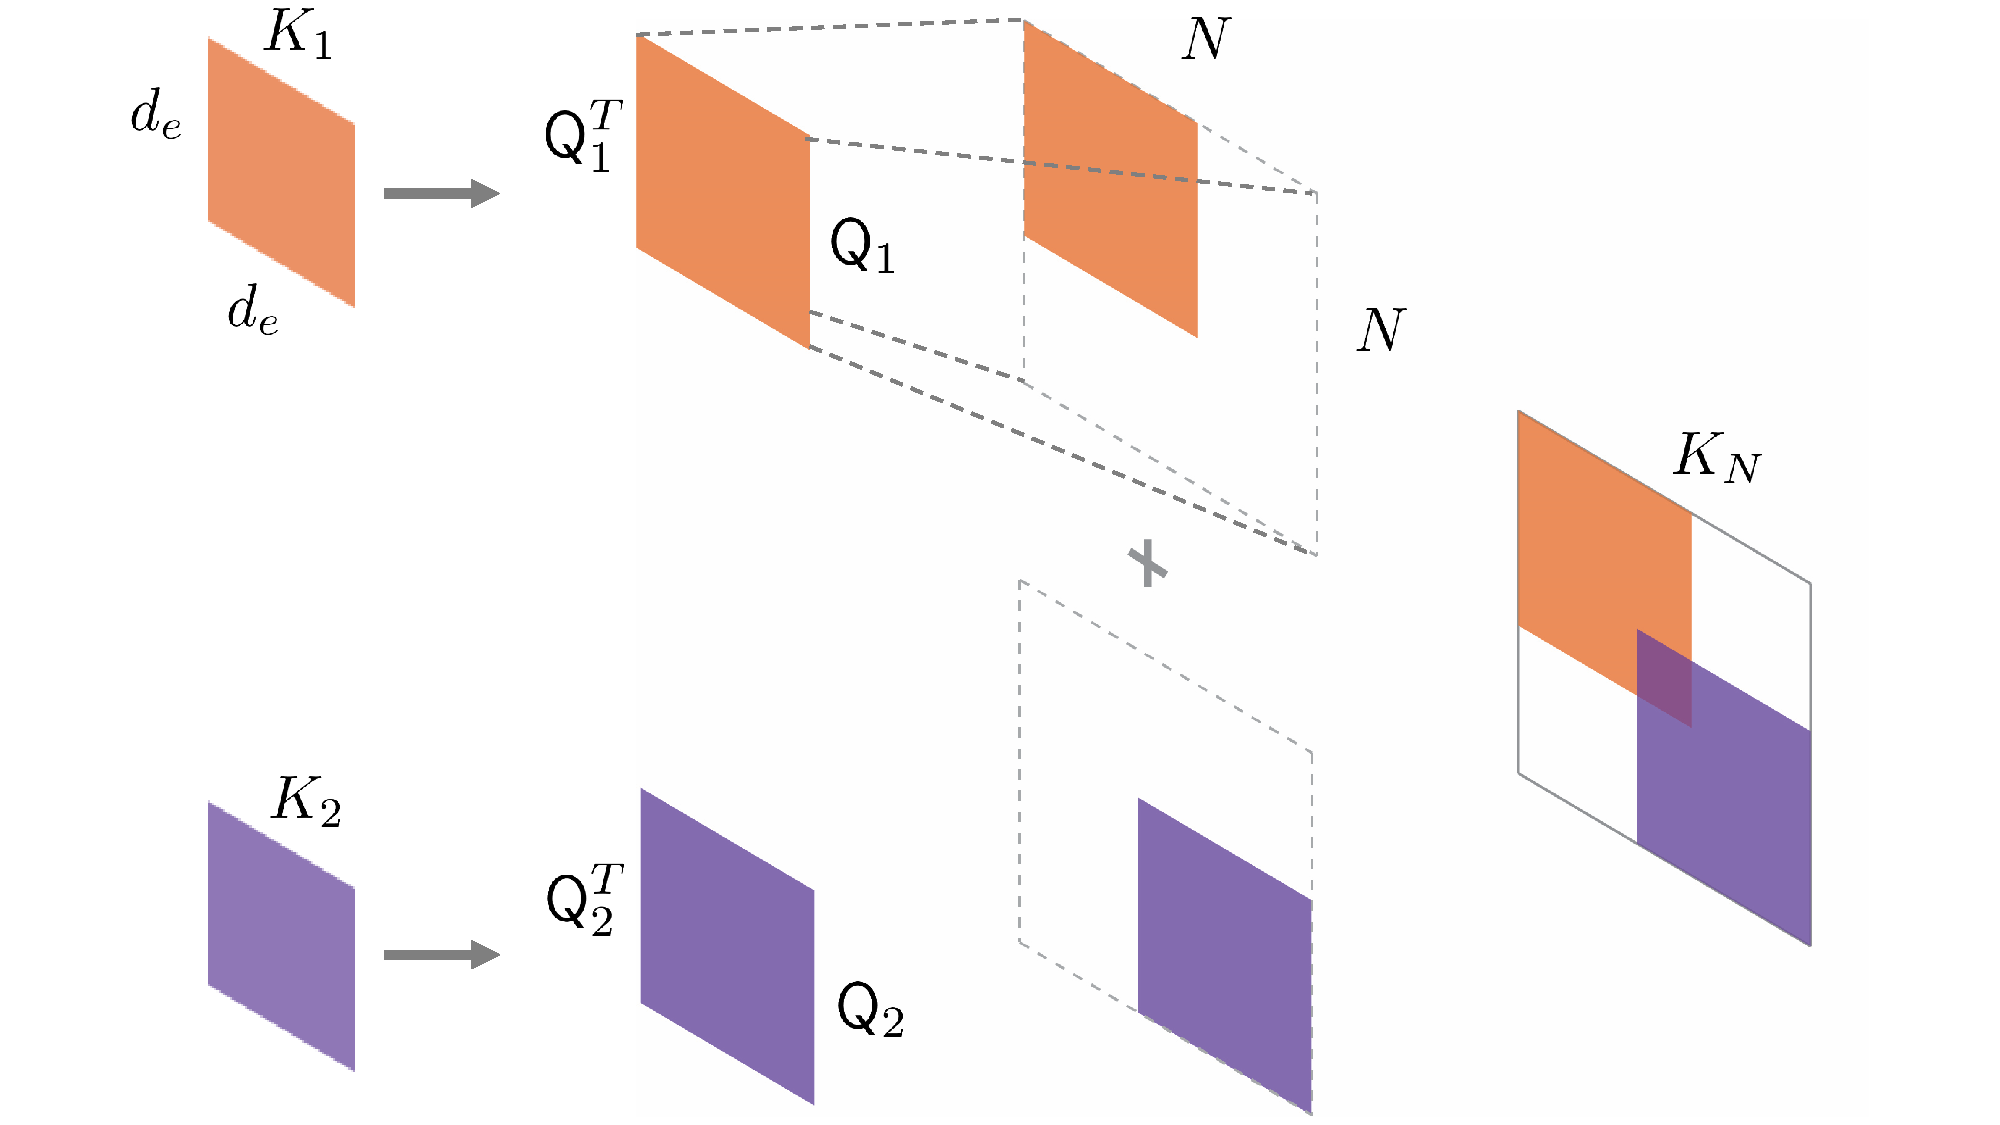
\includegraphics[width=0.6\linewidth]{K_full.pdf}
    \caption{Visual representation of the assembly of elemental stiffness matrices for the finite element model of the toy problem in Sec.~3. Local stiffness matrices \( \mat{K}_1 \) and \( \mat{K}_2 \), corresponding to individual finite elements, are transformed into the global coordinate system using their respective transformation matrices \( \mat{Q}_1 \) and \( \mat{Q}_2 \). These transformations expand the local matrices into the global framework, mapping local degrees of freedom to the global degrees of freedom. The global stiffness matrix \( \mat{K}_N \) is then constructed by adding these transformed matrices, summing contributions from overlapping degrees of freedom. Color-coded blocks highlight each local matrix's contribution to the global system.}
    \label{fig:visual_FOM_FEA}
\end{figure}


Here \( n_{\text{cell}} \) denotes the total number of cells or elements after meshing the domain \( \Omega \);  \( \Omega^e \) represent the domain of each cell; the \( \mat{K}^e\in\mathcal{R}^{d_e\times d_e} \) denotes the elemental stiffness matrix, with its $(i,j)$-th component defined as 

\begin{equation}
\mat{K}^e_{ij} = \int_{\Omega^{e}} k\left(\sum_{s=1}^{d_e} T_s \phi^e_s;\boldsymbol\mu\right) \nabla \phi^e_i \cdot \nabla \phi^e_j \, d\Omega^{e}
\label{eq:K_N_ij}
\end{equation}

and \( \vec{f}^e\in\mathcal{R}^{d_e} \) represents the elemental force vector, the $i-$th component of which is defined as
\begin{equation}
{f}^e_i = \int_{{\Omega}^e} q \phi_i \, d\Omega^{e}.
\label{eq:f_N_ij}
\end{equation}

where  \( d_e \) denotes the local degrees of freedom (DOF) of the \( e^{\text{th}} \) cell, the matrix \( \mat{Q}_e \) is a Boolean matrix of dimensions \( d_e \times N \), mapping the local DOFs \( d_e \) to the global DOFs \( N \) across the entire mesh (refer to \cref{fig:visual_FOM_FEA} for a visual representation).


We then solve \cref{eq:HC_HDM} for the coefficients \( \vec{T}_N \), and reconstruct the approximate temperature distribution \( T(x) \).
For the linear example, we assume the parametric linear thermal conductivity is given by
\begin{equation}
k(\mu) = 
\begin{cases} 
k_1 = \mu + 16, & \text{for} \quad 0.0 \leq x < 0.4   \\ 
k_2 = \mu + 30, & \text{for} \quad 0.4 \leq x \leq 0.5   
\end{cases}
\label{eq:k_mu_L}
\end{equation}
whereas for the nonlinear problem, the nonlinear thermal conductivity is defined as
\begin{equation}
k(T,\mu) = 
\begin{cases} 
k_1 =\mu + 16 + 2150/(T - 73.15),  &\quad 0.0 \leq x < 0.4 \\ 
k_1 =\mu + 30 + 2.09 \times 10^{-2} T - 1.45 \times 10^{-5} T^2 + 7.67 \times 10^{-9} T^3, & \quad 0.4 \leq x \leq 0.5 
\end{cases}
\label{eq:k_mu_NL}
\end{equation}

Additionally, the parametric internal heat generation is expressed as
\begin{equation}
q= 
\begin{cases} 
q_1(\beta) = \beta + 35000, & \text{linear, for} \quad 0.0 \leq x < 0.4 \\ 
q_1(T,\beta) = \beta + 35000 + T/10, & \text{nonlinear, for} \quad 0.0 \leq x < 0.4 \\ 
q_2(\beta) = 10\beta + 5000 & \text{(both) for} \quad 0.4 \leq x \leq 0.5 
\end{cases}
\label{eq:q_beta}
\end{equation}
Here both $\mu$ and $\beta$ are parameters.


We solve both the linear and the nonlinear problem for 32 pairs of $(\mu,\beta)$, where $\mu\in(-4,4)$ and $\beta\in(-1000,1000)$, using our native finite element code library using $5000$ 1D Lagrangian elements.
Though this problem does not require such fine mesh discretization, the dimension of the problem was artificially inflated to emulate a large-scale problem.


For the \textbf{linear} system, both $\vec{f}_N$ and $\mat{K}_N$ for different  parameter values were derived using \textit{affine decomposition} (see \cref{sec:glossary}).
Affine decomposition separates parameter dependence from spatial and temporal parts of a problem.
As a result, one can precompute and store parameter-independent components during an \textit{offline} phase, whereas in the \textit{online} phase, evaluate only parameter-dependent functions.
This saves the computational effort of iteratively evaluating $\vec{f}_N$ and $\mat{K}_N$ for different parameters.

For the linear problem, affine decomposition of  $\vec{f}_N$ and $\mat{K}_N$ is written as:

\begin{subequations}
\begin{align}
\mat{K}_N(\mu) &= \sum_{j=1}^2 k_j(\mu) \{\mat{K}^j_N\}_{\text{offline}} \\
\vec{f}_N(\beta) &= \sum_{j=1}^2 q_j(\beta) \{\vec{f}^j_N\}_{\text{offline}}
\end{align}
\label{eq:affine_Kb}
\end{subequations}


where $k_1(\mu)$, $k_2(\mu)$, $q_1(\beta)$, and $q_2(\beta)$ are purely parameter dependent, as in \cref{eq:k_mu_L,eq:q_beta}, and are calculated during the online phase; $\{\mat{K}^j_N\}_{\text{offline}}$ and $\{\vec{f}^j_N\}_{\text{offline}}$ are calculated offline assuming unit thermal conductivity and unit internal heat generation, and by assembling the elemental contributions from all cells associated with respective properties $k_j$ and $q_j$.
With Affine decomposition, the computational cost of many-query computations involving numerous parameter values is drastically reduced as the associated  computational effort grows linearly with the number of parameters.


For the \textbf{nonlinear} problem, however, an affine decomposition is not feasible because \(\vec{f}_N\) and \(\mat{K}_N\) must be evaluated individually for each parameter and iteratively during the solution of \(\vec{T}_N\) via Newton's method.
Consequently, solving the nonlinear problem is considerably more expensive.
While solving the linear problem across 32 parameters requires approximately 32 seconds of CPU time, the nonlinear problem demands around 500 seconds.
For both the linear and the nonlinear problems the parameters were selected using the Sobol scheme \cite{Sobol1967distribution} to ensure comprehensive coverage of the parameter space as shown in \cref{fig:HFS_HC_a,fig:HFS_HC_b}.
The corresponding solution snapshots for both problems are shown in \cref{fig:HFS_HC_c,fig:HFS_HC_d}.

\begin{figure}[t]
\centering
\begin{subfigure}[b]{0.45\linewidth}
\centering
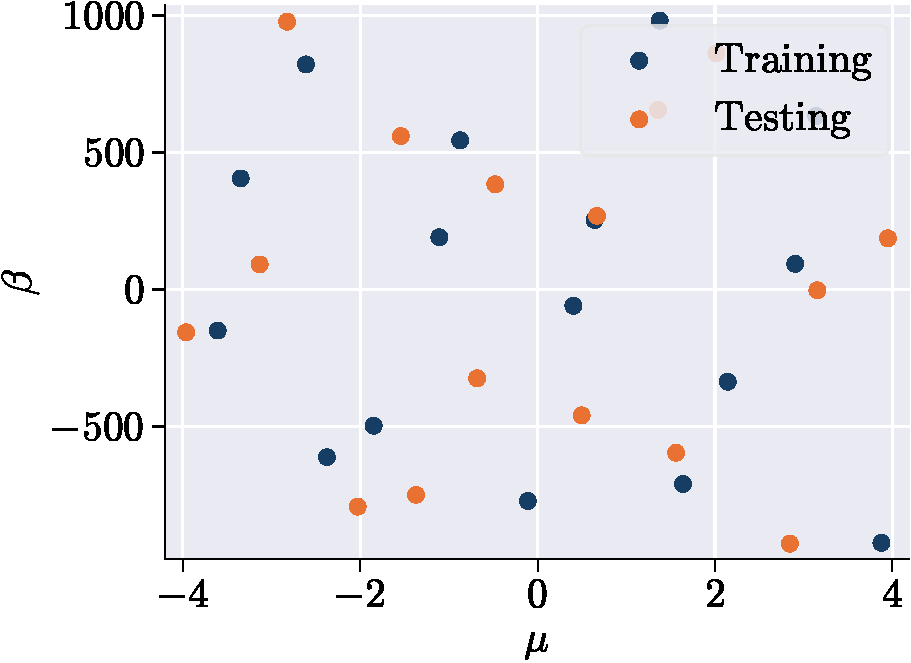
\includegraphics[width=\linewidth]{param_list_L.pdf}
\caption{}
\label{fig:HFS_HC_a}
\end{subfigure}
\begin{subfigure}[b]{0.45\linewidth}
\centering
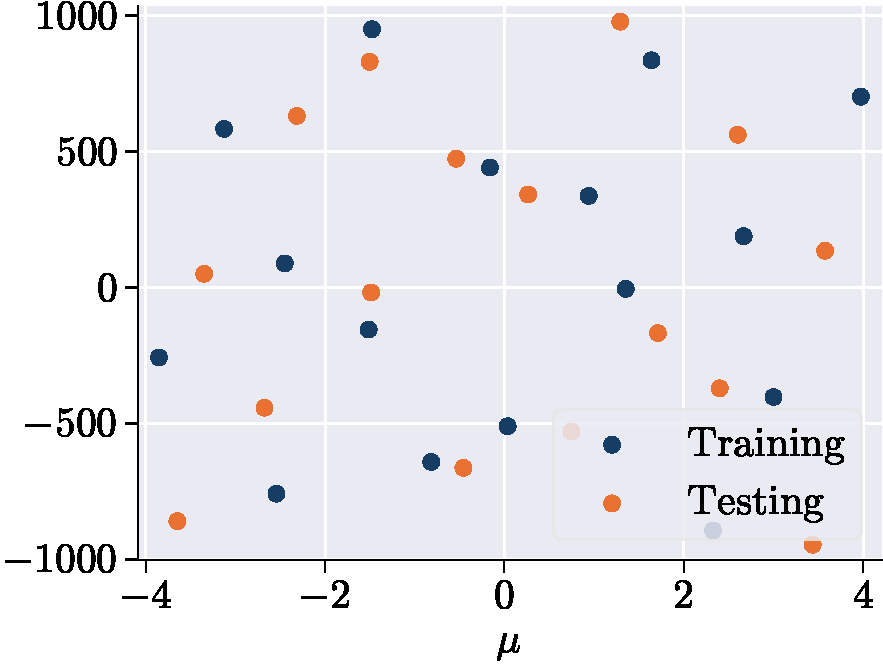
\includegraphics[width=0.98\linewidth]{param_list_NL.pdf}
\caption{}
\label{fig:HFS_HC_b}
\end{subfigure}

\begin{subfigure}[b]{0.45\linewidth}
\centering
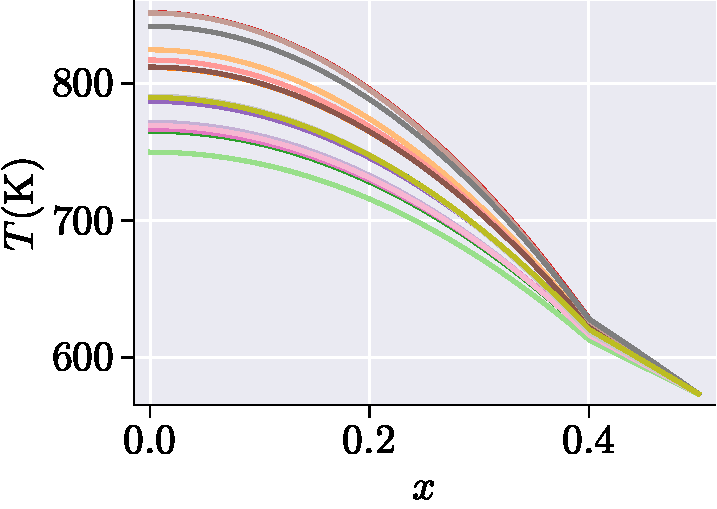
\includegraphics[width=\linewidth]{linear_T_FOM.pdf}
\caption{}
\label{fig:HFS_HC_c}
\end{subfigure}
\begin{subfigure}[b]{0.45\linewidth}
\centering
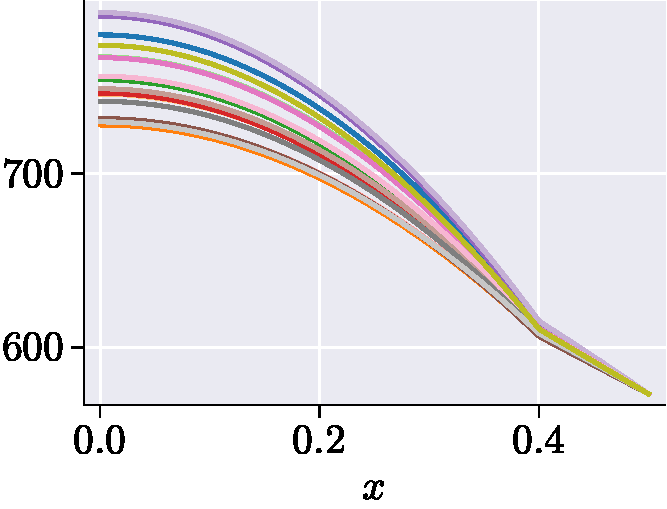
\includegraphics[width=0.92\linewidth]{nonlinear_T_FOM.pdf}
\caption{}
\label{fig:HFS_HC_d}
\end{subfigure}
\caption{High Fidelity solution snapshots for the linear and the nonlinear system corresponding to different values of the thermal conductivity and heat source values as defined in \cref{eq:k_mu_L,eq:k_mu_NL,eq:q_beta}.
Variation in the parameters for the linear system is shown in (a) and (c), and for the nonlinear system is shown in (b) and (d).
Here the parameter pairs are selected based on the sobol sequence, which explores the entire parameter space.}
\label{fig:HFS_HC}
\end{figure}

\begin{figure}[t]
\centering
\begin{subfigure}[b]{0.45\linewidth}
\centering
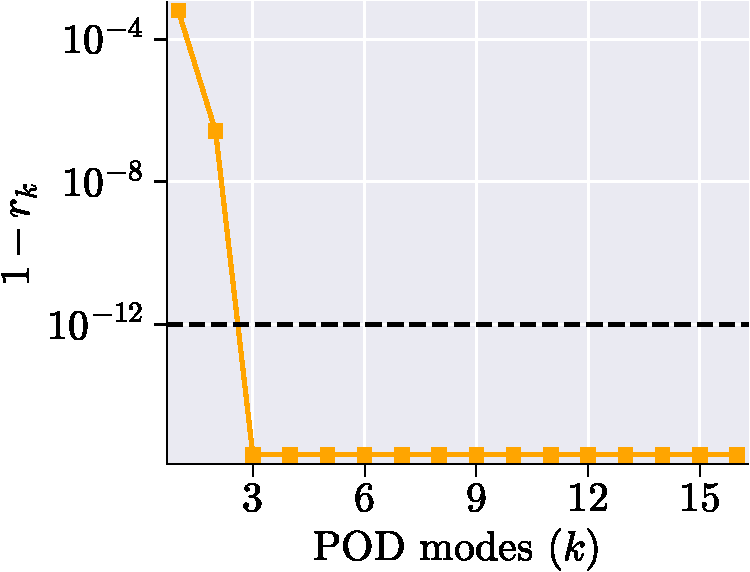
\includegraphics[width=\linewidth]{linear_Mode_selection.pdf}
\caption{}
\label{fig:HC_ROM_a}
\end{subfigure}
\begin{subfigure}[b]{0.45\linewidth}
\centering
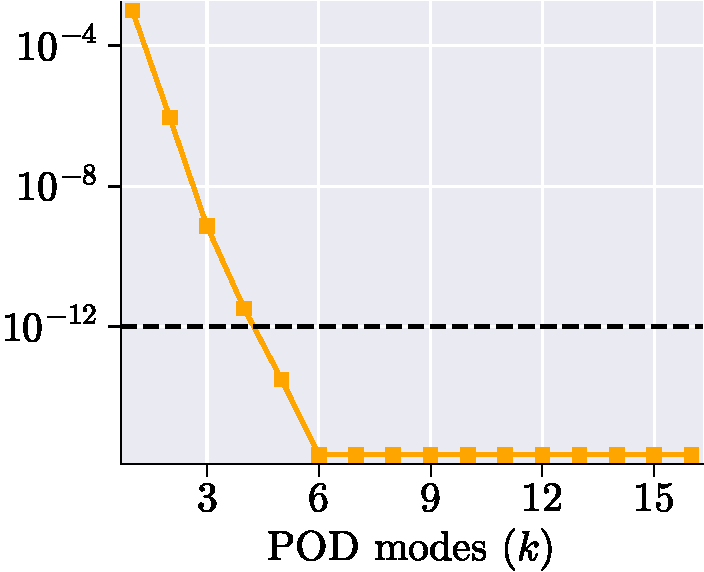
\includegraphics[width=0.93\linewidth]{nonlinear_Mode_selection.pdf}
\caption{}
\label{fig:HC_ROM_b}
\end{subfigure}

\begin{subfigure}[b]{0.45\linewidth}
\centering
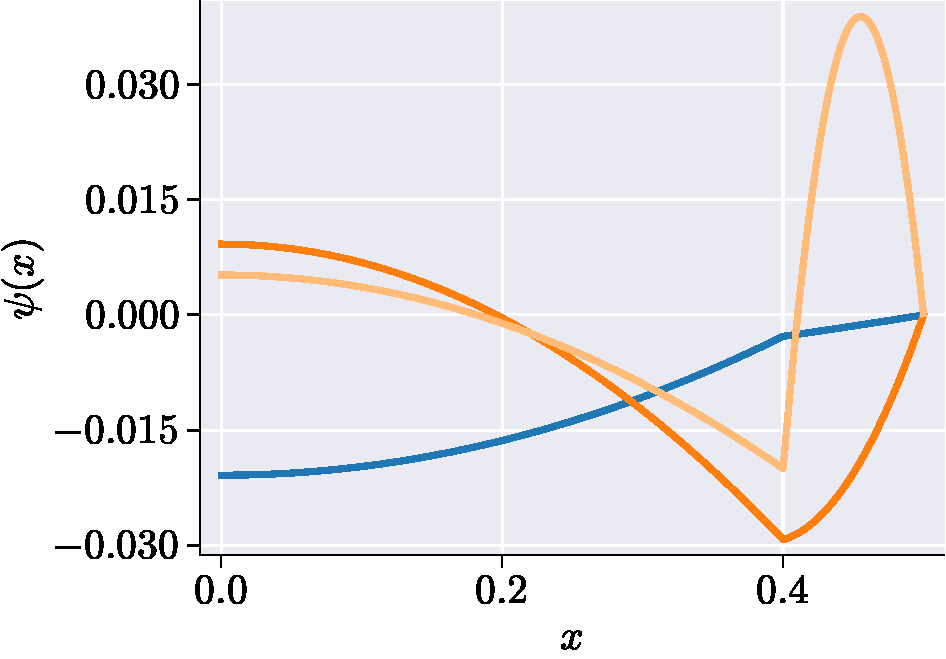
\includegraphics[width=\linewidth]{linear_Mode_shapes.pdf}
\caption{}
\label{fig:HC_ROM_c}
\end
{subfigure}
\begin{subfigure}[b]{0.45\linewidth}
\centering
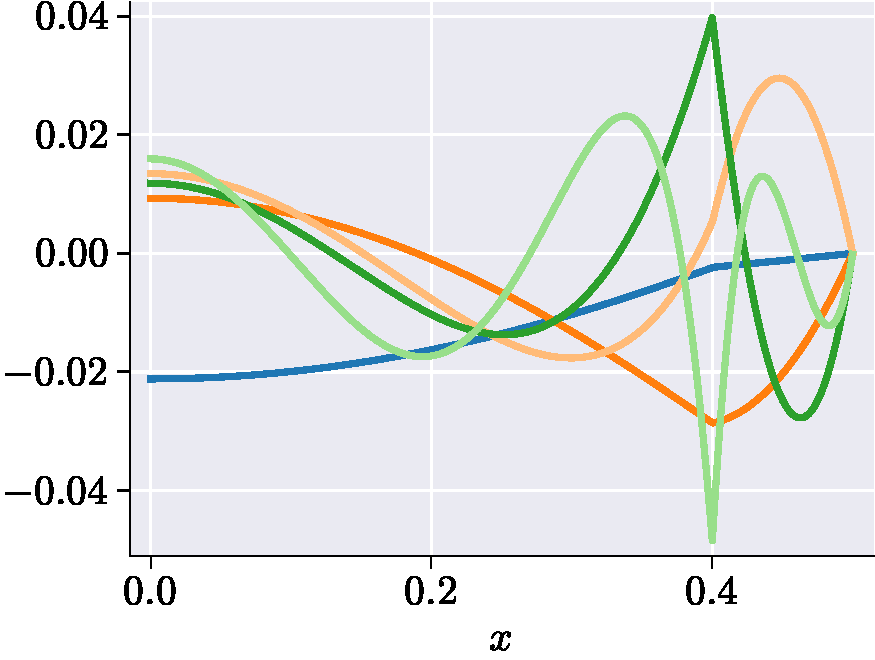
\includegraphics[width=0.96\linewidth]{nonlinear_Mode_shapes.pdf}
\caption{}
\label{fig:HC_ROM_d}
\end{subfigure}
\caption{Singular values and left reduced-order basis (ROB) obtained from the solution snapshots of  the linear (left column) and nonlinear (right column) problems.
Figures (a) and (b) display the decay of the singular values, with the dashed line indicating the chosen tolerance threshold, while (c) and (d) depict the corresponding spatial modes of the left ROB.}
\label{fig:HC_ROM}
\end{figure}







\begin{figure}[t]
\centering
\begin{subfigure}[b]{0.47\linewidth}
\centering
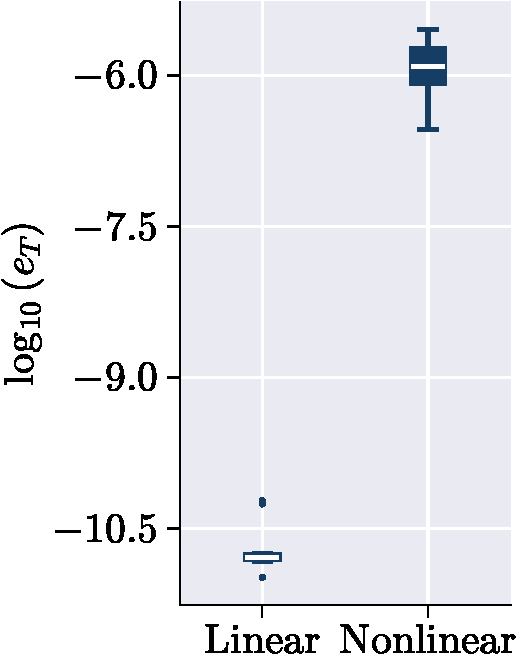
\includegraphics[height=0.95\linewidth]{error_comp.pdf}
\caption{}
\label{fig:HC_ERROR_SPDUP_c}
\end{subfigure}\hfill
\begin{subfigure}[b]{0.47\linewidth}
\centering
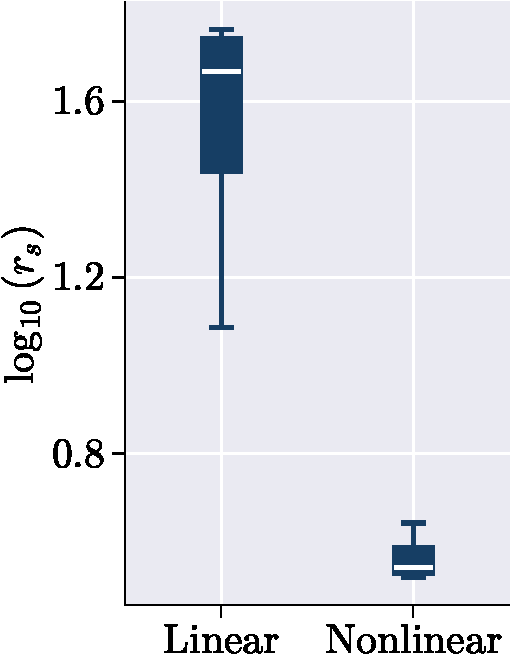
\includegraphics[height=0.95\linewidth]{speed_up_comp.pdf}
\caption{}
\label{fig:HC_ERROR_SPDUP_d}
\end{subfigure}
\caption{Difference in accuracy ($e_T$) and speed-up ($r_s$) between projection based linear and nonlinear ROMs.}
\label{fig:HC_ERROR_SPDUP}
\end{figure}



To obtain the reduced order models, POD was applied on the $50\%$ of the snapshots (treated as training data) and the dominant POD basis vectors, that span the reduced subspaces, were stored in $\mathbb{\widetilde{U}}$.
The number of basis vectors or the ROM dimension was selected by determining the minimum $k$, for which,  $1-r_k$ (Eq.~\ref{eq:mode_sel}), which indicates the fraction of the uncaptured data-variance for a $k$ dimensional subspace, was below a tolerance $\epsilon = 10^{-12}$, which yielded a three dimensional linear ROM ($n=3$) and a five dimensional nonlinear ROM ($n=5$) as shown in \cref{fig:HC_ROM_a,fig:HC_ROM_b}.
The corresponding modes selected are visualized in \cref{fig:HC_ROM_c,fig:HC_ROM_d}.


We express the approximate full order solution of \cref{eq:HC_HDM} as
\begin{equation}
\widehat{\vec{T}}_N = \overline{\vec{T}}_N + \mathbb{\widetilde{U}} \vec{T}_n
\label{eq:T_rec}
\end{equation}
where $\vec{T}_n$ denotes the reduced order solution and $\overline{\vec{T}}_N$ (equivalent to $\vec{w}^{ref}$ in \cref{eq:data_W}) represents the mean of the different temperature snapshots used for POD.
Then, following \cref{sec:ROM}, and assuming Galerkin projection, \cref{eq:HC_HDM} is reduced to
\begin{equation}
\mat{K}_n\vec{T}_n = \vec{f}_n- \widetilde{\mathbb{U}}^\top \mat{K}_N\overline{\vec{T}}_N 
\label{eq:HC_ROM}
\end{equation}
where

\begin{subequations}
\centering
\begin{align}
\vec{f}_n &= \mathbb{\widetilde{U}}^\top \vec{f}_N
\label{eq:f_red} \\
\mat{K}_n &= 
\begin{cases} 
\mathbb{\widetilde{U}}^\top \mat{K}_N(\mu) \mathbb{\widetilde{U}}, & \text{linear}   \\ 
\mathbb{\widetilde{U}}^\top \mat{K}_N(\widehat{\vec{T}}_N ;\mu ) \mathbb{\widetilde{U}}, & \text{nonlinear}
\end{cases}
\label{eq:K_red}
\end{align}
\label{eq:red_qoi}
\end{subequations}

For the linear problem, due to affine decomposition, the computation of $\mat{K}_n(\mu)$ and $\vec{f}_n(\beta)$ is  simple and fast since one can write:
\begin{subequations}
\begin{align}
\mat{K}_{n}(\mu) &= \sum_{i=1}^2 k_i(\mu) \widetilde{\mathbb{U}}^\top\{\mat{K}_i\}_{\text{offline}}\widetilde{\mathbb{U}} \\
\vec{f}_{n}(\beta) &= \sum_{j=1}^2 q_j(\beta) \widetilde{\mathbb{U}}^\top\{\vec{f}_j\}_{\text{offline}}
\end{align}
\label{eq:affine_Kb_rom}
\end{subequations}
The performance of the derived ROM was then tested using the remaining $50\%$ of the \textit{test} parameters and the corresponding snapshots.

As a measure of the ROM performance, we define the associated percentage relative error ($e_T$) and speed-up factor ($r_s$) as follows:
\begin{subequations}
  \begin{equation}
e_T = 100\times\dfrac{\|\vec{T}_{N}(\mu,\beta)_k-\widehat{\vec{T}}_N(\mu,\beta)_k\|_2}{\|\vec{T}_{N}(\mu,\beta)_k\|_2}
\label{eq:rom_error}
\end{equation}
where $\|\cdot\|_2$ indicates the $L_2$ norm; $(\mu,\beta)_k$ denotes the $k$th parameter pair, and
\begin{equation}
r_s = \dfrac{t_{HFM}}{t_{ROM}}
\label{eq:rom_speedup}
\end{equation}
\end{subequations}
where $t_{HFM}$ and $t_{ROM}$ indicate the total CPU-time required by the high-fidelity model and the reduced order model, respectively.
With $n=3$, for the test parameters, the linear ROM demonstrates high accuracy with $e_T\approx 10^{-10}$ and significant speed-up $r_s\approx 40$, as shown in \cref{fig:HC_ERROR_SPDUP_c,fig:HC_ERROR_SPDUP_d}.


For the nonlinear ROM, although the accuracy was quite reasonable, it was lower than in the linear case ($e_T = 10^{-6}$ compared to $10^{-10}$) (Although not shown, increasing $n$ was found to lower $e_T$).
More critically, the speed-up factor was substantially reduced: $4\times$ compared to $40\times$ in the linear case.
The primary reason for this reduced speed-up is evident from \cref{eq:K_red}, which indicates that the evaluation of the reduced stiffness matrix during the Newton iteration involves iterative evaluation of $\mat{K}_N$ and its projection onto the reduced subspace.
And for every evaluation, $\mat{K}_N$ requires the full-order solution $\widehat{\vec{T}}_N$, which is derived from $\vec{T}_n$ following \cref{eq:T_rec}.
Consequently, for nonlinear problems, regular projection-based reduced order models experience a significant decline in efficiency.



\section{Hyper-reduction techniques}





As discussed in the previous section, the efficiency of the projection-based ROMs is hindered by the need to iteratively map the reduced solutions back to the full-dimensional state to compute the solution-dependent non-linearities of the system and then again project them back to the reduced space. 
In this section, we introduce the idea of hyper-reduction, which offers efficient strategies to fast-compute the nonlinearities of a model with sufficient accuracy.



In general, nonlinearities can either be inherently polynomials, reducible to a polynomial form \cite{gu2011qlmor}, or non-polynomial in nature.
Consider the following example of polynomial nonlinearity written in Kronecker product form:
\begin{equation}
\mathbf{f}_N = \mat{K} \mathbf{w}_N + \mat{B} (\mathbf{w}_N \otimes \mathbf{w}_N) + \mat{C} (\mathbf{w}_N \otimes \mathbf{w}_N \otimes \mathbf{w}_N) + \dots
\label{eq:poly_non}
\end{equation}
where $\mat{K} \in \mathbb{R}^{N \times N}$, $\mat{B} \in \mathbb{R}^{N \times N^2}$, and $\mat{C} \in \mathbb{R}^{N \times N^3}$ are the coefficient tensors for the linear, quadratic, and cubic terms, respectively, and $\otimes$ denotes the Kronecker product \cite{kolda2009tensor}.

For an $n$-dimensional column vector $\mathbf{w}_N = [w_1, w_2, \dots, w_n]^\top$, the outer product $\mathbf{w}_N \otimes \mathbf{w}_N$ is defined as:

\begin{equation}
\mathbf{w}_N \otimes \mathbf{w}_N = [w_1^2, w_1w_2, \dots, w_1w_n, w_2w_1, w_2^2, \dots, w_2w_n, \dots, w_n^2] \in \mathbb{R}^{N^2}.
\label{eq:op}
\end{equation}


\begin{figure}
\centering
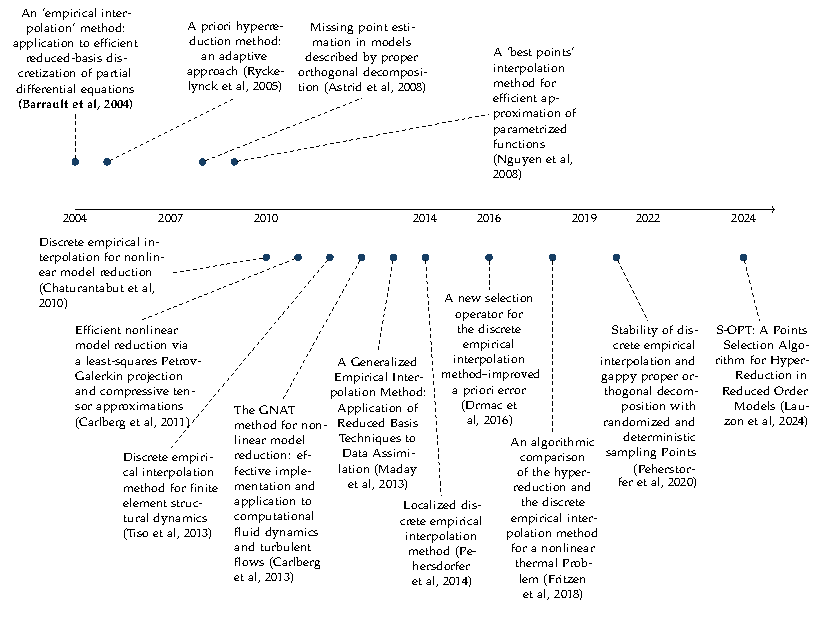
\includegraphics[width=\textwidth]{ATP.pdf}
\caption{Timeline of Seminal Papers on Approximate-then-Project hyper-reduction Algorithms. \cite{barrault2004empirical,ryckelynck2005priori,nguyen2007best,astrid2008missing,chaturantabut2010nonlinear,carlberg2011efficient,tiso2013discrete,carlberg2013gnat,peherstorfer2014localized,drmac2016new,peherstorfer2020stability,lauzon2024s-opt,Fritzen_2018,Maday_2013}.}
\label{fig:ATP_LIT}
\end{figure}

\begin{figure}[t]
    \centering
    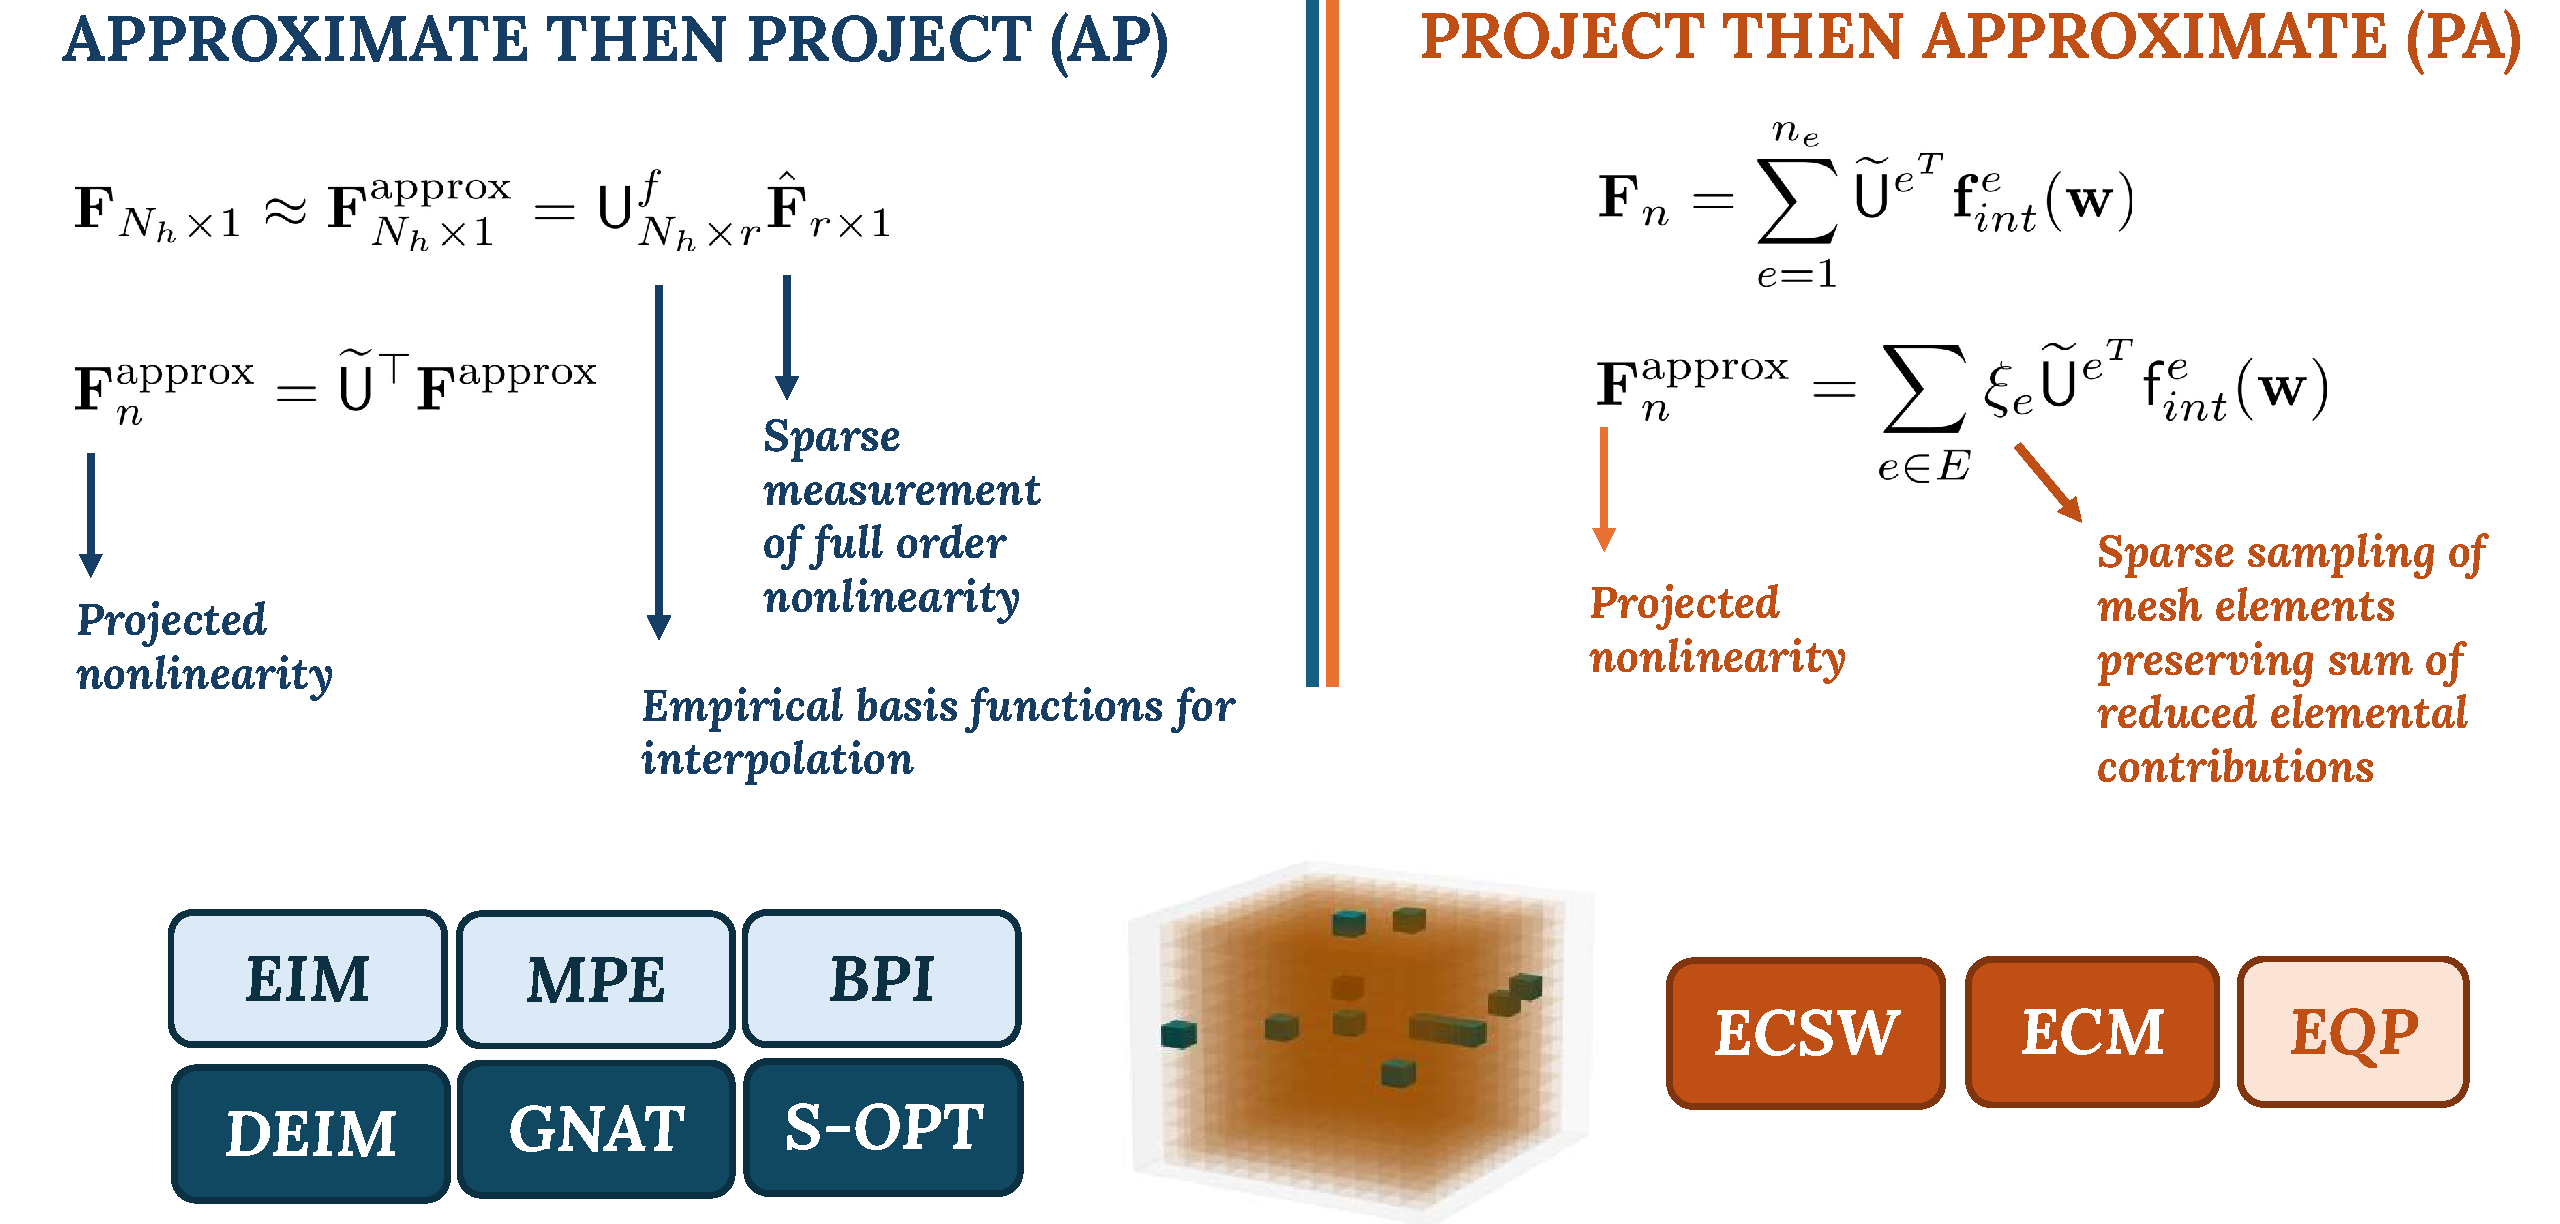
\includegraphics[width=\linewidth]{ATP_PTA2.pdf}
    \caption{Classification of hyper-reduction algorithms \protect\footnotemark(EIM: Empirical Interpolation Method \cite{barrault2004empirical}, MPE: Missing Point Estimation \cite{astrid2008missing}, BPI: Best Point Interpolation \cite{nguyen2007best}, DEIM: Discrete Empirical Interpolation Method \cite{chaturantabut2010nonlinear}, GNAT: Gauss-Newton Approximation Tensor \cite{carlberg2011efficient}, S-OPT: S-optimality based point selection \cite{lauzon2024s-opt}, ECSW: Energy Conserving Sampling and Weighing \cite{farhat2014dimensional}, ECM: Empirical Cubature Method \cite{hernandez2017dimensional}, EQP: Empirical Quadrature Procedure \cite{Patera_2017_EQP}): Approximate Then Project (AP) and Project Then Approximate (PA). In the AP approach, sparse measurements of the full-order nonlinearity are used in conjunction with empirical basis functions for interpolation, approximating the projected nonlinearity. In contrast, the PA approach involves projecting nonlinearity first and then employing sparse sampling of mesh elements to preserve the sum of reduced elemental contributions. Boxes with darker backgrounds, including DEIM, S-OPT, ECSW, and ECM are specifically discussed in the paper.}
    \label{fig:hyp_algo}
\end{figure}



The projection of $\mathbf{f}_N$ onto the reduced basis space $\mathbb{U}$ can then be expressed \textit{exactly} as \cite{ghattas2021learning}:
\begin{equation}
\widetilde{\mathbb{U}}^\top\vec{f}_N = \mathbf{f}_n =  \mat{K}_n \mathbf{w}_n + \mat{B}_n (\mathbf{w}_n \otimes \mathbf{w}_n) + \mat{C}_n (\mathbf{w}_n \otimes \mathbf{w}_n \otimes \mathbf{w}_n) + \dots
\label{eq:red_poly_non}
\end{equation}
where $\vec{w}_N=\widetilde{\mathbb{U}}\vec{w}_n$, and the reduced matrices are defined as:
\begin{equation}
\mat{K}_n = \widetilde{\mathbb{U}}^\top \mat{K} \widetilde{\mathbb{U}}, \quad \mat{B}_n = \widetilde{\mathbb{U}}^\top \mat{B} (\widetilde{\mathbb{U}} \odot \widetilde{\mathbb{U}}), \quad \mat{C}_n = \widetilde{\mathbb{U}}^\top \mat{C} (\widetilde{\mathbb{U}} \odot \widetilde{\mathbb{U}} \odot \widetilde{\mathbb{U}}),
\label{eq:red_matrices}
\end{equation}
and so on for higher-order terms.
The symbol \(\odot\) denotes the Khatri-Rao product (column-wise Kronecker product) of two matrices \cite{kolda2009tensor}.
For a matrix $\widetilde{\mathbb{U}} = [\vec{U}_1\, \vec{U}_2 \ldots \vec{U}_n] \in \mathcal{R}^{N \times n}$:
\begin{equation}
\widetilde{\mathbb{U}} \odot \widetilde{\mathbb{U}} = [\mathbf{U}_1 \otimes \mathbf{U}_1 \quad \mathbf{U}_2 \otimes \mathbf{U}_2 \quad \ldots \quad \mathbf{U}_n \otimes \mathbf{U}_n] \in \mathcal{R}^{N^2 \times n}.
\end{equation}
These reduced matrices $\mat{K}_n$, $\mat{B}_n$, and $\mat{C}_n$ can be precomputed, thereby eliminating the need to access the full order solution.


However in cases, where reduction to such a polynomial form is \textit{not} possible or preferred, and iterative access to full order solution is the only viable option to evaluate the nonlinear term, hyper-reduction is adopted.
Hyper-reduction focuses on scaling the computation with the size of the reduced coordinate vector $n$ rather than $N$, the size of the high-fidelity model (HFM).
This is achieved through sparse probing of the nonlinear terms across the computational domain, rather than calculating them at every nodal point. 
This approach is characterized by the use of a reduced mesh, where contributions from a significant portion of the mesh elements are omitted and accounted for through approximation. 
These methods introduce an additional layer of reduction on top of the projection-based reduction while maintaining the accuracy of the reduced-order model.


Hyper-reduction algorithms are classified under two major categories: approximate-after-project and project-after-approximate.
These names indicate the sequence of operations for handling nonlinearities.
In the approximate-after-project category, nonlinearities are first approximated within the full-dimensional space and then projected onto the reduced subspace.
Conversely, in the project-after-approximate category, this sequence is reversed.
In  \cref{fig:hyp_algo}, we show the different hyper-reduction algorithms widely used under each class.











In the remainder of this section, we introduce several widely employed algorithms along with their implementation details. 
Within the category of approximate-then-project methods, we examine the Discrete Empirical Interpolation Method (DEIM) and several DEIM-inspired algorithms. 
For project-then-approximate methods, we discuss the Energy Conserving Sampling and Weighing (ECSW) method and the Empirical Cubature Method (ECM).

\subsection{Approximate-then-project hyper-reduction strategies}

We begin by briefly introducing gappy-POD \cite{everson1995karhunen--loeve}, which was seminal in putting forward the idea behind the approximate-then-project hyper-reduction, and subsequently move onto describing the different hyper-reduction algorithms.
In \cref{fig:ATP_LIT} we present a brief timeline of the seminal papers on the approximate-then-project (AP) hyper-reduction algorithms.



\subsubsection{Gappy-Proper orthogonal decomposition (Gappy-POD)}
\label{sec:Gappy}

\noindent\hrulefill
\begin{itemize}
    \item {\bfseries Objective:} Reconstruct facial images using sparsely distributed pixels.
    \item Build a database containing complete images of various faces.
    \item Apply POD on the face database to construct an ``eigenfaces'' database.
    \item Reconstruct a new face approximately using the eigenfaces and partially available pixels of an out-of-sample image.
\end{itemize}
\noindent\hrulefill

The Gappy proper orthogonal decomposition (POD) method was developed in the context of facial image reconstruction from sparsely sampled pixels, given an already existing large database of grayscale images of different human faces \cite{sirovich1987low-dimensional}.


In the first step, proper orthogonal decomposition (POD) is applied to the entire facial image database to identify and express the most dominant facial features in the form of the proper orthogonal modes (POMs), which are termed as the \textit{eigenfaces}.
The subset of the most dominant eigenfaces are then utilized to approximate an image inside or outside  the dataset from a finite number of sampled pixels.
\Cref{fig:pic_db}a shows an example of a marred facial image with sparsely distributed pixels.
As discussed below, Gappy POD essentially reconstructed complete images from these sparse pixels by \textit{interpolating} with the eigenfaces.


Let a complete image be expressed as a $1$D vector $\vec{w}_N\in \mathcal{R}^{N\times 1}$, which contains the grayscale values at different pixel locations (obtained by reshaping the 2D image-matrix into 1D).
We define a sampling matrix $\mat{Z}\in \mathcal{R}^{N\times r}$, which samples a complete image at sparse locations to produce images as in \cref{fig:pic_db}a (sparse pixels on black background).
More formally, $\mat{Z}^{\top}$ projects the vector representation of a complete image, $\vec{w}_N$, onto an $r$-dimensional space, producing $\vec{w}_r$, which represents the marred image:
\begin{equation}
{\vec{w}}_r = \mat{Z}^{\top} \vec{w}_N
\end{equation}

As an example, $\mat{Z}$ may take the following form:

\begin{equation}
\mat{Z} =  
\begin{pmatrix}
1 & 0 & \cdots & 0\\
0 &  \vdots & \cdots &  \vdots \\
\vdots &  0 & \cdots &  1 \\
0 &  1 & 0 &  0 \\
\end{pmatrix}
\end{equation}
which has $r$ columns, with each column consisting of zeros except for a single element that is set to one, representing the specific pixel location being sampled.


For reconstruction, the image is expressed as the linear combination of the eigenfaces.
We write this as
\begin{equation}
\widetilde{\vec{w}}_N = \widetilde{\mathbb{U}}_f\vec{w}_n
\label{eq:rec_imag}
\end{equation}

where vector $\widetilde{\vec{w}}_N$ represents the reconstructed image, matrix $\widetilde{\mathbb{U}}_f\in \mathcal{R}^{N\times n}$ contains the first $n$ dominant eigenfaces reshaped into 1D vector of length $N$, and $\vec{w}_n\in\mathcal{R}^{n\times 1}$ is a vector containing the coefficients of $\widetilde{U}_f$.
It is enforced that the pixels of the marred image $\vec{w}_r$ match closely with the pixels of $\widetilde{\vec{w}}_N$ at the sampled location:
\begin{equation}
{\vec{w}}_r \approx \mat{Z}^{\top}\widetilde{\mathbb{U}}_f\vec{w}_n
\end{equation}
such that $\vec{w}_n$ minimizes the  reconstruction error:

\begin{equation}
   \vec{w}_n = \arg\min_{\vec{w}_n} \| \vec{w}_r - \mat{Z}^{\top}\widetilde{\mathbb{U}}_f\vec{w}_n \|_2
   \label{eq:sampling_optimization}
\end{equation}
where $\|\cdot\|_2$ denotes the $L_2$ norm.


The normal equation for this optimization problem is given by
\begin{equation}
 {\vec{w}_n} = \left(\mat{Z}^{\top}\widetilde{\mathbb{U}}_f\right)^{\dagger}\vec{w}_r = \Omega^{-1}\mat{Z}^{\top}\widetilde{\mathbb{U}}_f\vec{w}_r
\label{eq:solution_ak}
\end{equation}
where $^{\dagger}$ denotes the pseudo-inverse and $\Omega = \left(\widetilde{\mathbb{U}}_f^{\top}\mat{Z}\mat{Z}^{\top}\widetilde{\mathbb{U}}_f\right)$.
Subsequently, the complete image is reconstructed using \cref{eq:rec_imag}.
Figs.~\ref{fig:pic_db}b and~\ref{fig:pic_db}d show the images reconstructed from the pixels in Fig.~\ref{fig:pic_db}a.
The reconstructed images look reasonably close to the true image shown in Fig.~\ref{fig:pic_db}c.



\begin{figure}[t!]
    \centering
    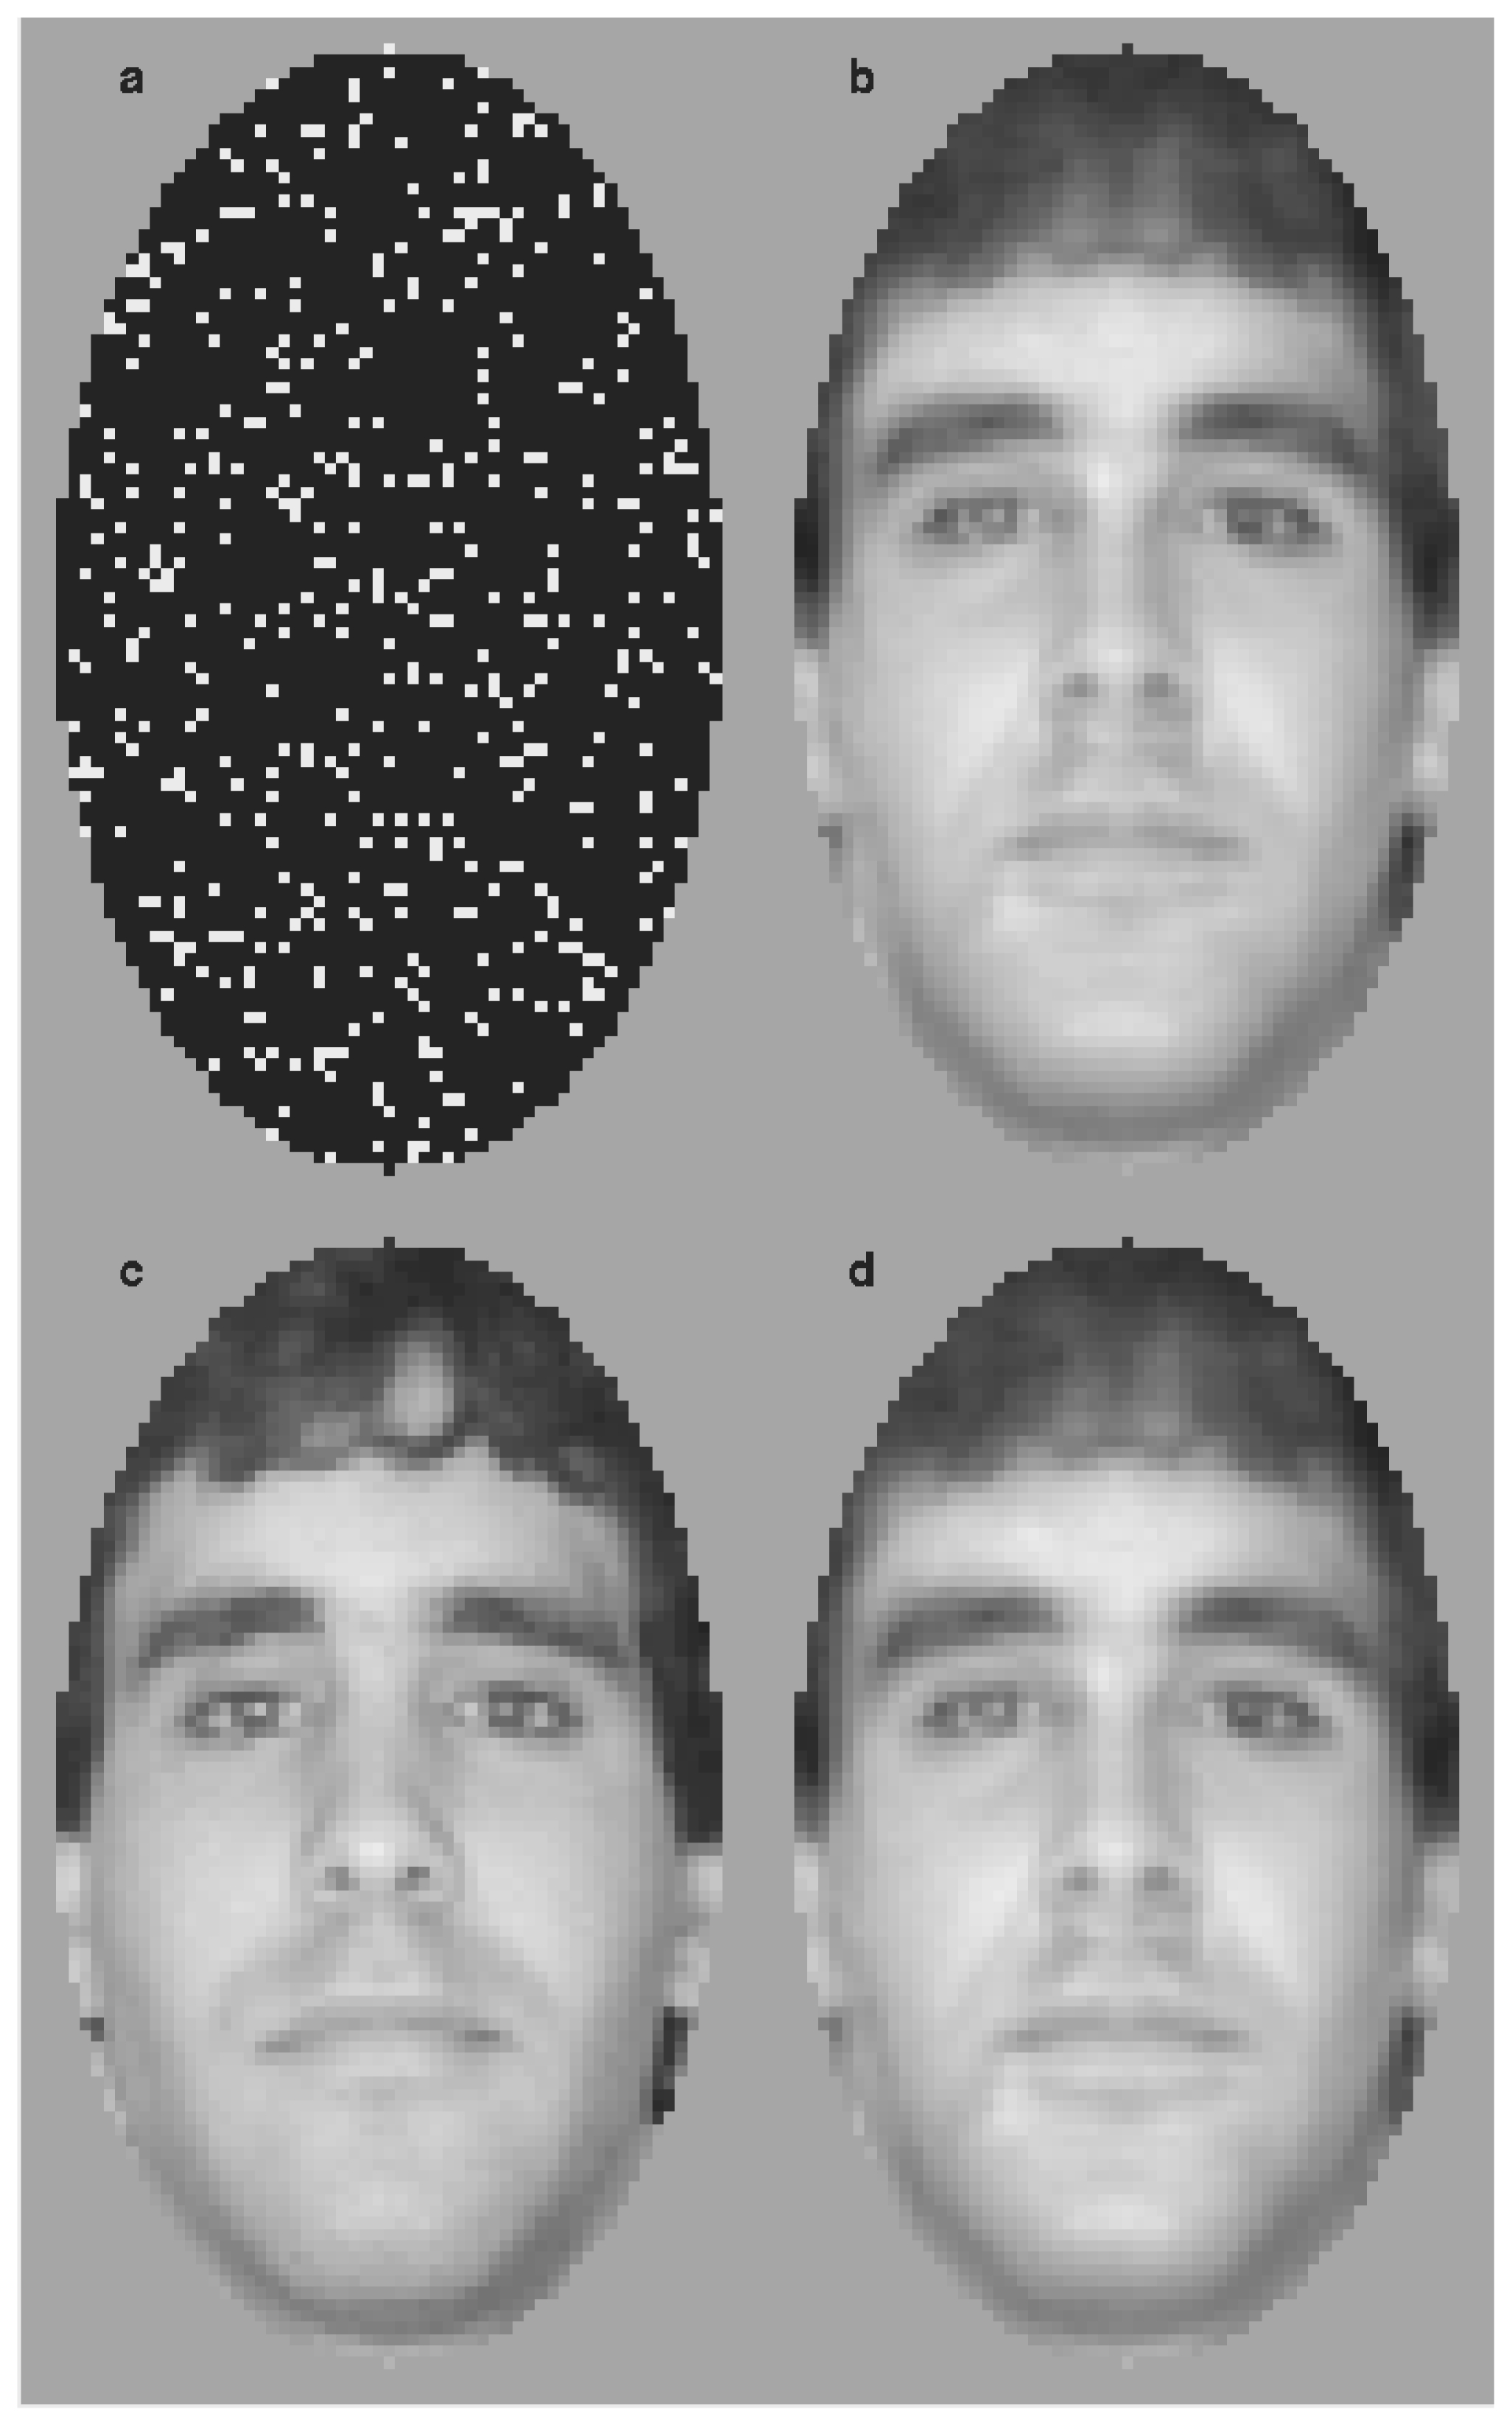
\includegraphics[width=0.25\linewidth]{gappy_pod2.jpg}
    \caption{Reconstruction of marred images using Gappy-POD \cite{sirovich1987low-dimensional}.}
\label{fig:pic_db}
\end{figure}


\remark Note that the columns of $\mat{Z}^{\top}\widetilde{\mathbb{U}}_f$ contain the row-wise sampled columns of $\widetilde{\mathbb{U}}_f$.
Unlike the columns of $\widetilde{\mathbb{U}}_f$, which are the basis vectors, these columns are sampled basis vectors and hence are not orthonormal, and hence, $\mat{\Omega}$ is not an identity matrix.
However, as the sampling space becomes  denser, then $\mat{\Omega} \to \mat{I}_n$.
As a matter of fact, the efficacy of gappy-POD depends upon the condition number of $\mat{\Omega}$.
If the image sampling is such that resulting $\mat{\Omega}$ has a large condition number, which indicates $\mat{\Omega}$ is close to being singular and non-invertible, the reconstructed image may deviate significantly from the original image.
Further details on how sampling affects the condition number can be found in Ref.~\cite{brunton2019data-driven}.
However, with a proper sampling matrix $\mat{Z}$, which yields lower (preferably, close to unity) condition number for $\Omega$, it may be possible to achieve reasonably accurate reconstruction of an image from a limited number of pixels.
This very idea is leveraged in the AP hyper-reduction algorithms, as we will discuss next.


\subsubsection{Discrete empirical interpolation method (DEIM)}
    
\noindent\hrulefill
\begin{itemize}
    \item {\bfseries Objective:} Determine interpolation points on the computational domain associated with a High-Fidelity Model (HFM) to approximate a nonlinear term and reduce computational complexity.
    \item Gather snapshots of system state variables over time or training parameters and apply POD to construct a reduced basis for the HFM.
    \item Collect snapshots of the nonlinear term and apply POD  to construct a reduced basis specific to the nonlinear term.
    \item Select interpolation points that maximize information retention in the nonlinear term using the POD basis from its snapshots.
    \item Approximate the nonlinear term in the ROM by evaluating it at selected points and reconstructing it with the reduced basis, bypassing full-order complexity.
\end{itemize}
\noindent\hrulefill




The Discrete Empirical Interpolation Method (DEIM), introduced in \cite{chaturantabut2010nonlinear}, was developed to efficiently compute the projected nonlinearity, such as $\vec{f}_n$ in \cref{eq:ROM_eq}, by approximating the full-order nonlinear term, such as $\vec{f}_N$ in \cref{eq:gov_eq}, via a low-dimensional representation constructed from a set of reduced basis vectors and carefully chosen sampling locations.
The approach is very similar to Gappy POD.
However, unlike Gappy POD, which reconstructs full images from a \textit{given} incomplete image data, DEIM \textit{selects} specific components (sampling/interpolation points) of the nonlinear force vector according to a sampling strategy.

\subsubsection*{DEIM approximation framework}
\begin{algorithm}[t]
\caption{Discrete Empirical Interpolation Method: Offline Phase \cite{Hesthaven2016,chaturantabut2010nonlinear}}
\begin{algorithmic}[1]
\STATE \textbf{function} $[\mathbf{Q}, \mathcal{J}, \mathbf{Z}] = \text{DEIM\_OFFLINE}(\mat{F}, tol)$
\STATE $[\vec{U}_f^1, \dots, \vec{U}_f^r] = \text{POD}(\mat{F}, tol)$ \textcolor{blue}{// Perform POD on force snapshots $\mat{F}$, obtaining $r$ basis vectors based on tolerance \textit{tol}}
\STATE $i_1 = \arg\max_{i=1,\dots,N} |\vec{U}_f^1|_i$ \textcolor{blue}{// Select the index of the maximum absolute entry in the first POD basis vector}
\STATE $\mat{Q} = \vec{U}_f^1$, $\mathcal{J} = \{ i_1 \}$ \textcolor{blue}{// Initialize basis matrix $\mat{Q}$ and index set $\mathcal{J}$ with the first POD basis vector and index}
\STATE $\mat{Z} = [\vec{e}_{i_1}]$ \textcolor{blue}{// Initialize sampling matrix $\mat{Z}$ with the standard basis vector corresponding to $i_1$}
\FOR{$m = 2 : r$}
    \STATE Compute $\mathbf{\tilde{q}} = \mat{Q} (\mat{Z}^\top \mat{Q})^{\dagger} \mat{Z}^\top \vec{U}_f^m$ \textcolor{blue}{// Project the current POD basis vector $\vec{U}_f^m$ onto the span of accumulated basis vectors in $\mat{Q}$, using $\mat{Z}$ for row selection}
    \STATE $\mathbf{r} = \vec{U}_f^m - \mathbf{\tilde{q}}$ \textcolor{blue}{// Calculate the residual between $\vec{U}_f^m$ and its projection}
    \STATE $i_m = \arg\max_{i \notin \mathcal{J}} |\mathbf{r}|_i$ \textcolor{blue}{// Select index of the maximum absolute entry in the residual that is not in $\mathcal{J}$}
    \STATE $\mathbf{Q} \leftarrow [\mat{Q} \, \vec{U}_f^m]$, $\mathcal{J} \leftarrow \mathcal{J} \cup \{ i_m \}$ \textcolor{blue}{// Update basis matrix $\mat{Q}$ and index set $\mathcal{J}$ with the new POD basis vector and index}
    \STATE $\mat{Z} \leftarrow [\mat{Z} \, \vec{e}_{i_m}]$ \textcolor{blue}{// Append the standard basis vector for $i_m$ to $\mat{Z}$, updating the sampling matrix}
\ENDFOR
\STATE \textbf{end function}
\end{algorithmic}
\label{alg:DEIM_offline}
\end{algorithm}


Given a parametric nonlinear vector $\vec{f}_N: \overline{\Omega} \times \mathcal{P}_{\text{DEIM}} \to \mathcal{R}^N$, where \( \overline{\Omega} \) is the spatial domain and \( \mathcal{P}_{\text{DEIM}} \) is the parameter space, DEIM approximates \( \vec{f}_N \) using a given set of basis vectors \( \widetilde{\mathbb{U}}_f \in \mathbb{R}^{N \times r} \) and the values of $\vec{f}_N$ at specific sampling points.
The approximation, denoted by $\widehat{\vec{f}}_N$, is expressed as
\begin{equation}
    \widehat{\vec{f}}_N(\vec{w}^{\boldsymbol{\mu}}; \boldsymbol{\mu}) = \widetilde{\mathbb{U}}_f \left(\mat{Z}^\top \widetilde{\mathbb{U}}_f\right)^{\dagger} \mat{Z}^\top \vec{f}_N(\vec{w}^{\boldsymbol{\mu}}; \boldsymbol{\mu}) = \mat{M}_D \vec{f}_N(\vec{w}^{\boldsymbol{\mu}}; \boldsymbol{\mu})
    \label{eq:deim_approx}
\end{equation}

where the sampling matrix $\mat{Z}$ contains the sampling locations, and $\mat{M}_D$  defined as
\begin{equation}
 M_D = \widetilde{\mathbb{U}}_f \left(\mat{Z}^\top \widetilde{\mathbb{U}}_f\right)^{\dagger} \mat{Z}^\top
 \label{eq:deim_mat}
\end{equation}
is an oblique projection matrix (see \cref{sec:glossary}).
It can be seen that \Cref{eq:deim_approx} follows directly from \cref{eq:solution_ak,eq:rec_imag}.


This approximation is subsequently used to calculate the projected nonlinearity $\widehat{\vec{f}}_n$ for \cref{eq:ROM_eq}:
\begin{equation}
    \widehat{\vec{f}}_n  = \widetilde{\mathbb{U}}^\top \, \widehat{\vec{f}}_N
    \label{eq:deim_approx_fn}
\end{equation}
where $\widetilde{\mathbb{U}}$ contains the reduced basis vectors derived from the solution snapshots (Eq.~\ref{eq:U_tilde}).


DEIM derives its basis vectors \( \widetilde{\mathbb{U}}_f \in \mathbb{R}^{N \times r} \) by directly applying SVD to the snapshot matrix consisting of snapshots of \( \vec{f}_N(\vec{w}^{\boldsymbol{\mu}_q}; \boldsymbol{\mu}_q) \) , which we will refer to as DEIM-snapshots, for each \( \boldsymbol{\mu}_q \in \mathcal{P}_{\text{DEIM}} \):
\begin{equation}
\mat{F} = \left[ \vec{f}_N(\vec{w}^{\boldsymbol{\mu}_1}; \boldsymbol{\mu}_1), \cdots, \vec{f}_N(\vec{w}^{\boldsymbol{\mu}_{N_s}}; \boldsymbol{\mu}_{N_s}) \right] \approx \widetilde{\mathbb{U}}_f \mat{\Sigma}_f \mathbb{V}_f^\top.
\end{equation}
The left singular vectors corresponding to the first $r$ largest singular values form the columns of \( \widetilde{\mathbb{U}}_f \).


The error associated with the approximation in \cref{eq:deim_approx} is bounded as  \cite{chaturantabut2010nonlinear}:
\begin{equation}
    \|\vec{f}_N - \widehat{\vec{f}}_N\|_2 \le \|\left(\mat{Z}^\top \widetilde{\mathbb{U}}_f\right)^{\dagger}\|_2 \, \| (\mat{I}-\widetilde{\mathbb{U}}_f\widetilde{\mathbb{U}}_f^{\top})\vec{f}_N\|_2
    \label{eq:deim_error}
\end{equation}

where \(\|\vec{f}_N - \widehat{\vec{f}}_N\|_2\) denotes the Euclidean norm of the approximation error.
The term \(\|\left(\mat{Z}^\top \widetilde{\mathbb{U}}_f\right)^{\dagger}\|_2\) reflects the sensitivity to the selected sampling points, where \((\cdot)^{\dagger}\) is the pseudo-inverse.
As discussed in \cref{sec:Gappy}, a large value of this term indicates a poor condition number of  $\mat{Z}^\top \widetilde{\mathbb{U}}_f$, which in turn indicates that the sampling points may not be quasi-optimal (true optimality cannot be achieved in general due to dependence on \(\vec{f}_N\)).
Finally, the term \(\|(\mat{I} - \widetilde{\mathbb{U}}_f \widetilde{\mathbb{U}}_f^{\top}) \vec{f}_N\|_2\)  denotes the projection error, which quantifies the residual portion of \(\vec{f}_N\) not captured by the span of reduced basis \(\widetilde{\mathbb{U}}_f\).

In DEIM, the approximation error is reduced by reducing  $\|\left(\mat{Z}^\top \widetilde{\mathbb{U}}_f\right)^{\dagger}\|_2$ on the right-hand side by maximizing its smallest singular value $\sigma_{\text{min}}\left(\mat{Z}^\top \widetilde{\mathbb{U}}_f\right)$, which in turn minimizes the condition number $\kappa = {\sigma_{\text{max}}\left(\mat{Z}^\top \widetilde{\mathbb{U}}_f\right)}/{\sigma_{\text{min}}\left(\mat{Z}^\top \widetilde{\mathbb{U}}_f\right)}$ ensuring that $\left(\mat{Z}^\top \widetilde{\mathbb{U}}_f \right)$ is invertible.
The DEIM algorithm as described in \cref{alg:DEIM_offline} achieves this via an appropriate construction of the sampling matrix $\mat{Z}$.

This greedy \cref{alg:DEIM_offline} selects sampling points by iteratively searching for the index where the residual $\vec{r}$ (step 8) is maximum, thereby limiting the step-wise growth of $\|\left(\mat{Z}^\top \widetilde{\mathbb{U}}_f\right)^{\dagger}\|_2$ and minimizing $\kappa$, ensuring invertibility.
In essence, this process results in the selection of \( r \) independent \textit{rows} of \( \mathbb{\widetilde{U}}_f \).

\remark
DEIM reduces complexity of calculating $\vec{f}_N$ from \( \mathcal{O}(N) \) to \( \mathcal{O}(r) \), enabling efficient handling of large-scale problems.

\remark
Computation of $\vec{f}_N$ using \cref{eq:deim_approx} for any $\boldsymbol{\mu}\in\mathcal{P}_{\text{DEIM}}$ during the online phase is accelerated by the offline computation of $\mat{M}_D$ in \cref{eq:deim_mat}, commonly referred to as the DEIM-matrix.

\remark
By selecting $\mat{Z}$ that maximizes $\sigma_{\text{min}}\left(\mat{Z}^\top \widetilde{\mathbb{U}}_f\right)$, the DEIM algorithm achieves \textit{E-optimality} \cite{Pukelsheim2006,lauzon2024s-opt}, reducing the maximum approximation error defined in \cref{eq:deim_error}.


\remark
Discrete Empirical Interpolation Method (DEIM) is a discrete adaptation of its predecessor Empirical Interpolation Method (EIM), as outlined in \cref{sec:algorithms}. 
EIM focuses on interpolating nonlinear \textit{functions} by simultaneously constructing empirical basis functions and determining sampling nodes in an iterative manner for a quasi-optimal representation of the nonlinear function. 
In contrast, DEIM decouples these steps in a discrete framework by first applying Singular Value Decomposition (SVD) to the DEIM snapshots to generate basis functions, and then selecting the indices.

\subsubsection*{Implementation on the running example problem}

 Consider the nonlinear heat conduction problem in Section \ref{sec:ROM_example}.
We use the same training and test datasets each containing 16 parameter pairs, $(\mu, \beta)_k$ for $k=1, \ldots, 16$, to formulate and evaluate DEIM-based hyper-reduced order models (hyper-ROMs).
The POD basis matrix, $\widetilde{\mathbb{U}}$, in this case is constructed using $4$ basis vectors.


To implement \cref{alg:DEIM_offline} during the offline phase, we started by gathering snapshots of the source term \( q \) for each set of training parameters.
Since the steady-state heat conduction problem reduces to a root-finding problem of the residual, selecting either the source term itself or the product of the stiffness matrix $\mat{K}_N$ with the solution yields equivalent DEIM snapshots.
\Cref{fig:DEIM_snap_a} visualizes the spatial variation of the source term over different parameter values, while \cref{fig:DEIM_snap_b} shows the singular value decay of the DEIM snapshots, which informs the selection of the reduced basis size \( r \) for constructing \( \mathbb{U}_f \in \mathcal{R}^{N \times r} \).
We selected \( r = 4 \) (though \cref{fig:DEIM_snap_b} suggests $r=3$ would also suffice), which results in 4 DEIM points.
This led to a section of 8 elements out of a total of 5000, as each node in the 1D mesh (excluding boundaries) is shared by two elements.
This is shown in \cref{fig:reduced_mesh_deim}.
The DEIM sampling algorithm then generated the DEIM matrix \( \mathsf{M}_D \) as in \cref{eq:deim_mat}, facilitating efficient evaluations of both the right-hand and left-hand sides of \cref{eq:HC_HDM}.
The dimension of the reduced solution subspace $n$ was also chosen to be $4$ (See Remark 5 for the rationale).


In \cref{fig:HROM_ERROR_SPDUP_deim}, we compare the computational speed-up (Eq.~\ref{eq:rom_speedup}) and the relative percentage error (Eq.~\ref{eq:rom_error}) between the hyper-ROM and the conventional projection-based ROM.
As shown in \Cref{fig:HROM_ERROR_SPDUP_a_deim}, the hyper-ROM achieves a relative error of 0.001\%, which, although slightly higher than that of the regular ROM, is accompanied by a substantial computational speed-up—nearly 30 times that of the regular ROM.


\begin{figure}[t]
\centering
\begin{subfigure}[b]{0.45\linewidth}
\centering
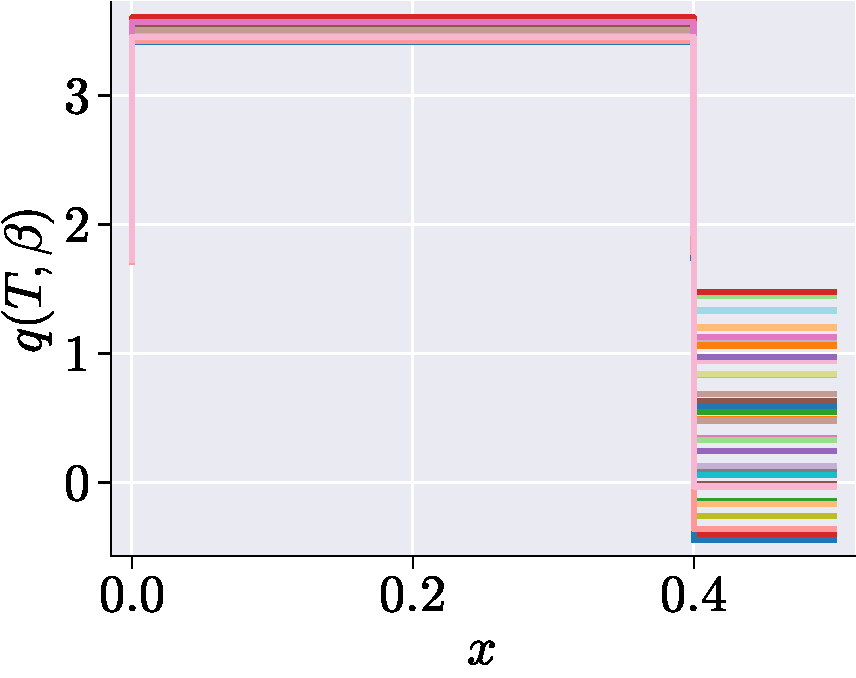
\includegraphics[width=\linewidth]{DEIM_snapshots.pdf}
\caption{}
\label{fig:DEIM_snap_a}
\end{subfigure}
\begin{subfigure}[b]{0.45\linewidth}
\centering
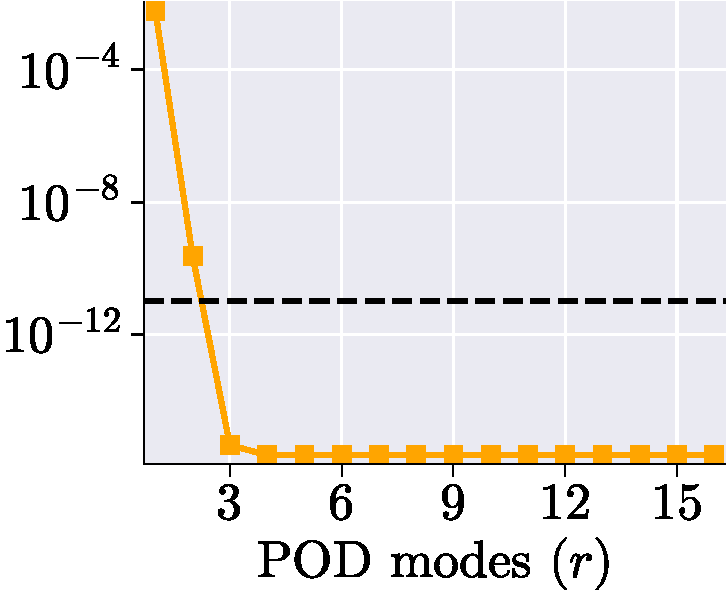
\includegraphics[width=0.97\linewidth]{DEIM_SVs.pdf}
\caption{}
\label{fig:DEIM_snap_b}
\end{subfigure}
\caption{The snapshots of the source function corresponding to various parameter values used for DEIM are shown in (a).
In (b), the decay of singular values, obtained by applying SVD on the snapshots, is illustrated.
This decay informs the selection of the number of singular vectors, \( r \), to use in the DEIM algorithm.
Here, \( r = 4 \) was selected.}
\label{fig:DEIM_snap}
\end{figure}

\begin{figure}[t]
    \centering
    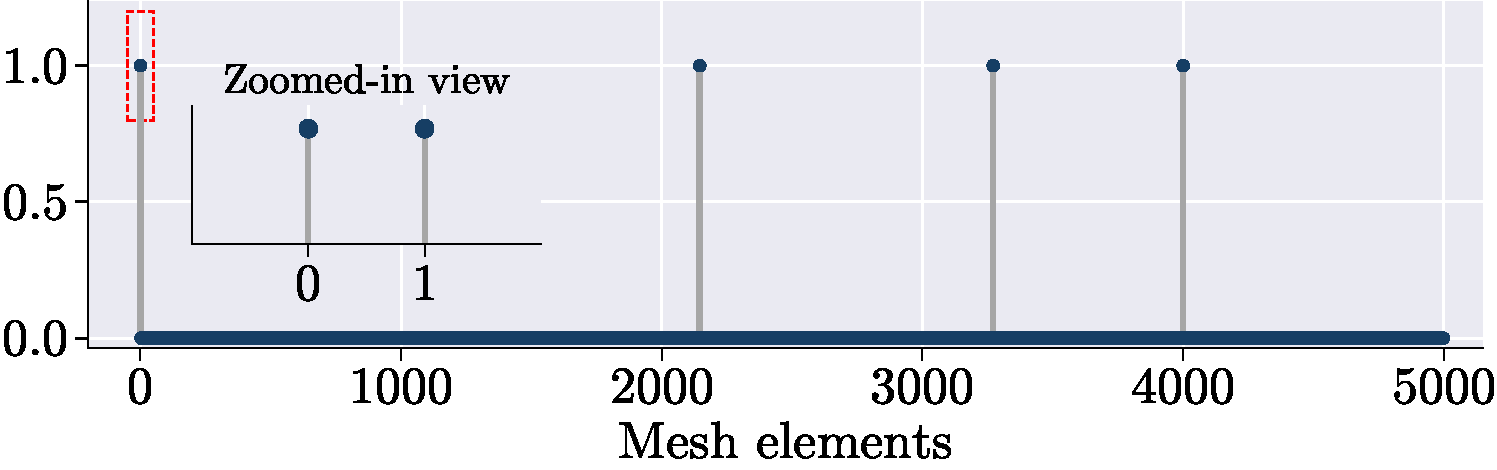
\includegraphics[width=0.8\linewidth]{reduced_mesh_DEIM_new.pdf}
    \caption{The reduced mesh obtained using DEIM. Excluded  elements lie on the blue line. As shown in the inset, for each DEIM point, all associated elements (in this case, two per point) are selected. The resulting reduced mesh in this case comprises only 8 elements, which constitutes 0.16\% of the total 5,000 elements in the original high-fidelity model.}
    \label{fig:reduced_mesh_deim}
\end{figure}

\begin{figure}[t!]
\centering
\begin{subfigure}[b]{0.47\linewidth}
\centering
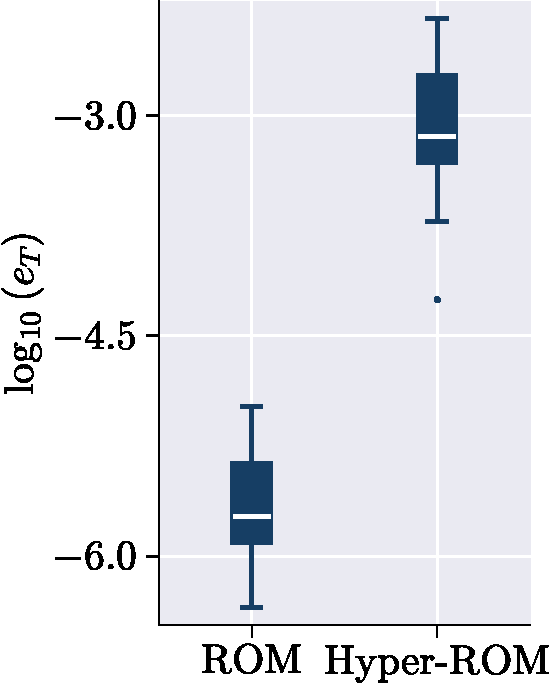
\includegraphics[height=0.95\linewidth]{error_comp_rom_hrom_deim.pdf}
\caption{}
\label{fig:HROM_ERROR_SPDUP_a_deim}
\end{subfigure}\hfill
\begin{subfigure}[b]{0.47\linewidth}
\centering
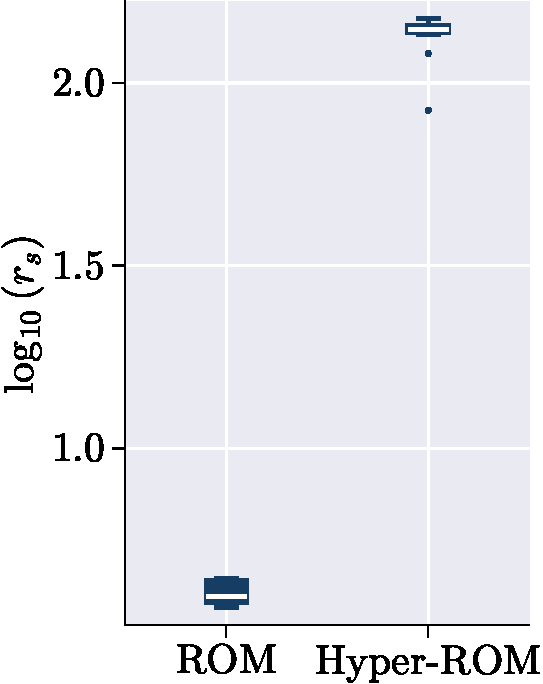
\includegraphics[height=0.95\linewidth]{speed_up_comp_rom_hrom_deim.pdf}
\caption{}
\label{fig:HROM_ERROR_SPDUP_b_deim}
\end{subfigure}
\caption{Difference in accuracy ($e_T$) and speed-up ($r_s$) between the regular projection based ROM and Hyper-ROM.}
\label{fig:HROM_ERROR_SPDUP_deim}
\end{figure}



\remark
In DEIM-based hyper-reduction, instability often results from selecting an inconsistent number of modes for DEIM ($r$) and solution snapshots ($n$), leading to non-invertible projected quantities.
To maintain stability in the reduced-order model, it is  recommended that the number of solution modes should not exceed the number of singular vectors obtained from the DEIM snapshots, i.e.
$n\le r$.
This rationale informed our choice to set $r = n = 4$ in our example problem.
We observed that increasing $n$ further leads to instability.
Moreover, singular values associated with the DEIM snapshots for $r>4$ are so small that the corresponding singular vectors are essentially noise and also leads to instability.

\remark
If the DEIM snapshots exhibit limited variability, the number of singular vectors available for selection will be small, constraining the reduced dimension and, consequently, the accuracy of the hyper-reduced model.
To achieve a stable and accurate ROM, it is essential to ensure adequate variation in the DEIM snapshots, allowing for a larger set of singular vectors and a robust reduced representation.


\subsubsection{Alternative algorithms similar to DEIM}

Over time, several (D)EIM-inspired alogorithms have been developed to address specific challenges and improve performance.
Notable among these are Q-DEIM, Localized DEIM (LDEIM), Unassembled DEIM (U-DEIM), and S-OPT.
\paragraph{Q-DEIM} The Q-DEIM (QR-based Discrete Empirical Interpolation Method) \cite{drmac2016new} improves upon the traditional DEIM algorithm by using QR decomposition with column pivoting to select interpolation points.
A key numerical linear algebra question motivating Q-DEIM is whether one can construct an sampling matrix \( Z \) that ensures the condition number of the DEIM projection remains moderate, regardless of the chosen orthonormal basis \( \widetilde{\mathbb{U}}_f \).
Traditional DEIM is sensitive to the specific basis of singular vectors, especially when singular values are closely clustered or repeated, which can lead to instability and variable interpolation quality.
Q-DEIM addresses this issue by determining interpolation points independently of any specific orthonormal basis through QR factorization with column pivoting.
This approach provides a priori assurance of a moderate condition number for the DEIM projection, enhancing numerical stability and reducing errors.
As a result, Q-DEIM offers a robust and efficient method for constructing the interpolation matrix \( S \), making it particularly suitable for applications like sensor placement in sparse interpolation contexts where reliable interpolation point selection is crucial.
\paragraph{LDEIM} Localized DEIM (LDEIM), enhances the DEIM approach by employing multiple local subspaces instead of a single global subspace for approximating the nonlinear term \cite{peherstorfer2014localized}.
This method is particularly advantageous in problems where the nonlinear term varies greatly over different regions.
LDEIM accomplishes this by using machine learning-based clustering algorithms to discover the regions that should form each local subspace.
During the online phase, classification-based machine learning methods are then used to adaptively select the appropriate local subspace for the DEIM approximation.
While the additional computational overhead of LDEIM may not be justified for problems where the nonlinear term behaves relatively uniformly, it has been demonstrated to provide substantial benefits in cases with large variation in the nonlinear term.
In such scenarios, LDEIM can achieve speedups of up to two orders of magnitude compared to traditional DEIM algorithms.
\begin{figure}[t]
    \centering
    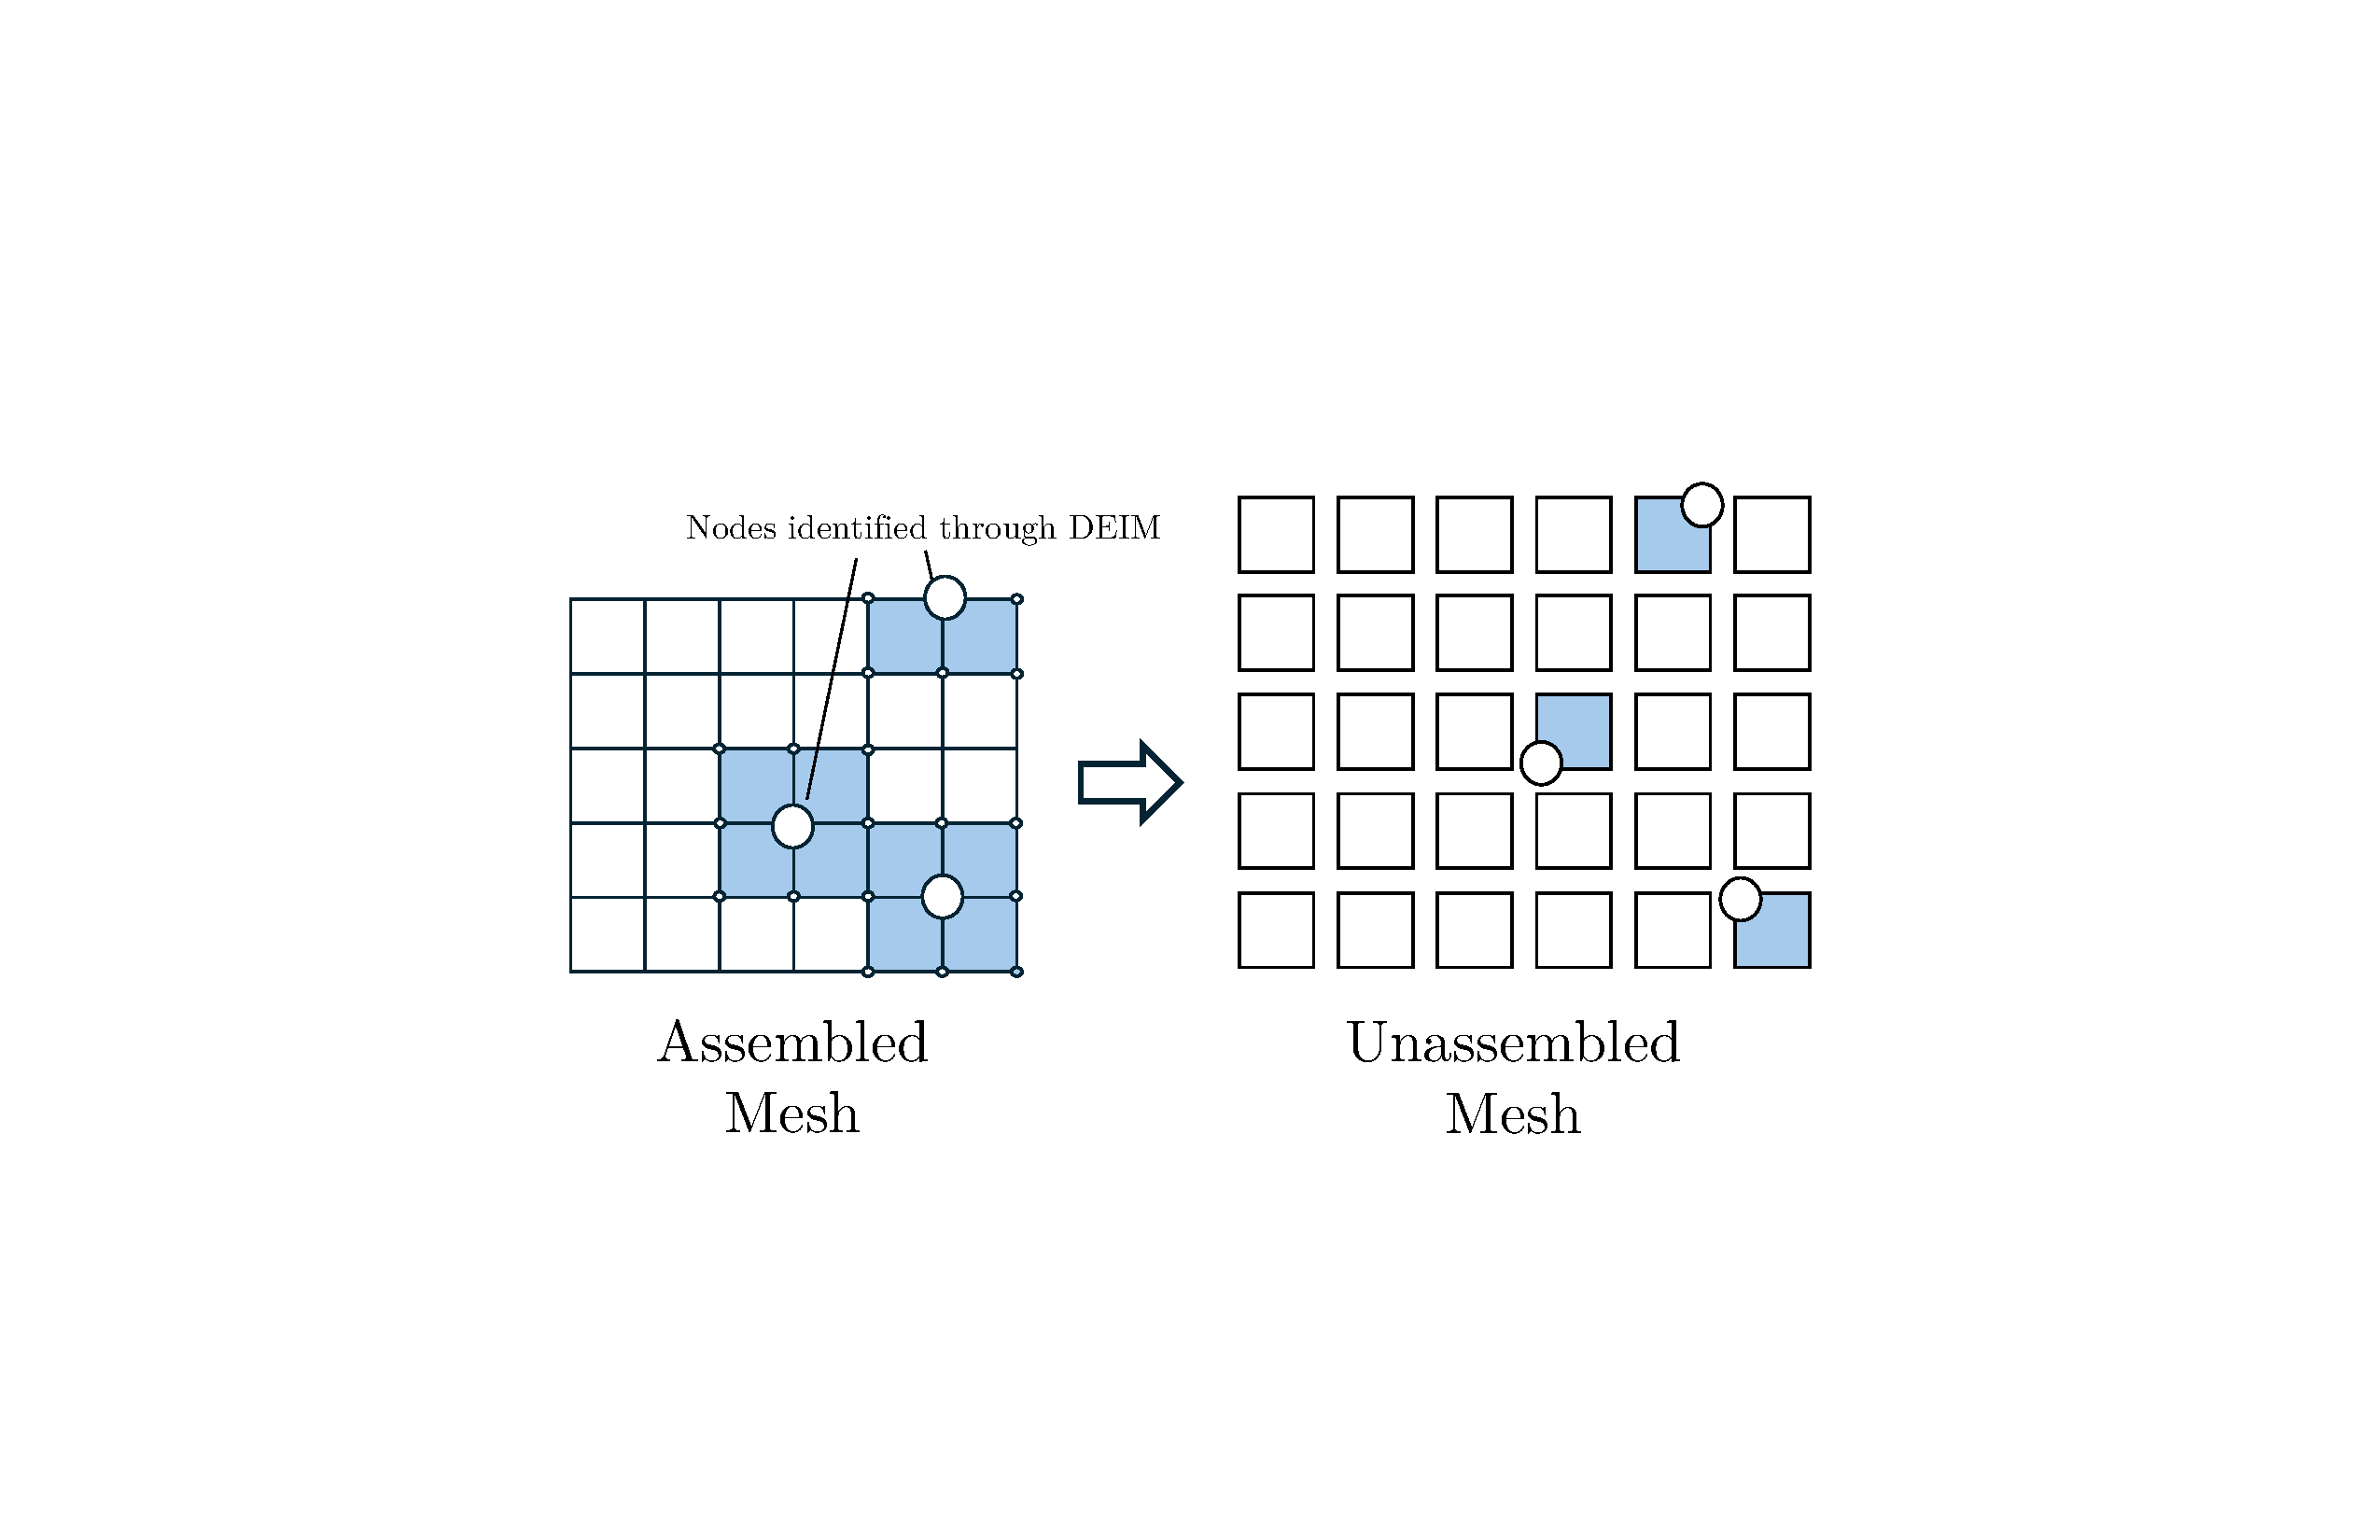
\includegraphics[width=0.7\linewidth]{udeim2.pdf}
    \caption{Unsassembled DEIM requires less elements to be sampled than the traditional DEIM algorithm for Finite Element problems. (Adapted from \cite{tiso2013discrete})}
    \label{fig:UDEIM}
\end{figure}
\paragraph{U-DEIM} Unassembled DEIM (U-DEIM) improves the applicability of DEIM to simulations using the Finite Element Method (FEM) \cite{tiso2013discrete}.
It can be difficult to efficiently apply DEIM to FEM simulations because nodes in FEM can be shared by multiple elements (as was seen for the example toy problem as well).
If a node is selected with the typical DEIM algorithm, it will require the contributions of all adjacent elements to be calculated.
This greatly increases the number of elements required, which decreases the efficiency of DEIM.
U-DEIM solves this problem by applying the DEIM approximation to the unassembled form of the FEM system.
This means only the contributions from one element are required to calculate the DEIM approximation.

The difference between the assembled and unassembled DEIM is illustrated in \cref{fig:UDEIM}, where there is a significant decrease in the number of elements included in the U-DEIM case.
After the DEIM approximation is calculated, the force matrix can be assembled in the same way it is done in typical FEM.
U-DEIM is more efficient to calculate for FEM problems than the traditional DEIM method.
However, U-DEIM comes with a trade-off: the system matrix assembled with U-DEIM is not symmetric, which leads to instability in the solution of the nonlinear system.
There are strategies to mitigate this instability, but they do not completely eliminate it.
U-DEIM is a good option for FEM problems where efficiency is valued highly enough to overcome the possible instability present in the method.
\paragraph{S-OPT} S-OPT, or S-optimality method was originally introduced by Shin and Xiu as a stochastic collocation method for uncertainty quantification \cite{shin2016SOPT}.
Its application to hyper-reduction was later explored in \cite{lauzon2024s-opt}.


Similar to DEIM, S-OPT aims to construct a sampling matrix $\mat{Z}$, which reduces the function approximation error described in \cref{eq:deim_error} by reducing $\|\left(\mat{Z}^\top \widetilde{\mathbb{U}}_f\right)^{\dagger}\|_2$.


Recalling \cref{eq:solution_ak}, we write:
\begin{equation}
\left(\mat{Z}^{\top}\widetilde{\mathbb{U}}_f\right)^{\dagger} = \Omega^{-1}\mat{Z}^{\top}\widetilde{\mathbb{U}}_f
\label{eq:sopt_error}
\end{equation}
where $\dagger$ denotes the pseudo-inverse and $\Omega = \left(\widetilde{\mathbb{U}}_f^{\top}\mat{Z}\mat{Z}^{\top}\widetilde{\mathbb{U}}_f\right)$.
As discussed in \cref{sec:Gappy}, the magnitude of the pseudo-inverse in \cref{eq:sopt_error} decreases when (a) the determinant of $\Omega$ is large in mangitude, which will ensure its invertibility and (b) the columns of $\left(\mat{Z}^\top \widetilde{\mathbb{U}}_f\right)$ are orthogonal.


The S-OPT achieves both objectives simultaneously by constructing a $\mat{Z}$ that maximizes a scalar function $\mathscr{S}$ of $\left(\mat{Z}^\top \widetilde{\mathbb{U}}_f\right)$, defined as

\begin{equation}
    \mathscr{S}(\mat{P}) = \left( \frac{\sqrt{|\det \left( \mat{P}^\top \mat{P}\right)}|} {\Pi_{i=1}^r \|\mat{P}[:,i]\|}\right)^{\frac{1}{r}}
\end{equation}
where $\mat{P}=\mat{Z}^\top {\mat{Q}}_f$, and $\mat{Q}_f$ is obtained from the QR decompostion of $\widetilde{\mathbb{U}}_f=\mat{Q}_f\mat{R}$.
Here $\mat{P}[:,i]$ denotes the $i$th column of $\mat{P}$.
The maximization problem is written as

\begin{equation}
\mat{Z}^*_{\text{S-OPT}} = \underset{\mat{Z}  \in \mathbb{R}^{N \times n}}{\arg\max} \, \mathscr{S}(\mat{Z}^\top \mat{Q})
\label{eq:sopt_max}
\end{equation}
The S-OPT algorithm,  detailed in \cref{alg:S_OPT} yields a quasi-optimal solution to this maximization problem.


Using Hadamard's inequality \cite{hadamard1893}, it can be shown that $\mathscr{S} \in [0,1]$.
The inequality states that for any symmetric matrix $\mat{M}$
\begin{equation} 
|\det(\mat{M})| \leq \prod_{i=1}^{p} M_{ii}, 
\end{equation}
with equality holding only when the columns of $\mat{M}$ are orthogonal.
Here, $M_{ii}$ denotes the $i$th diagonal entry of $\mat{M}$.
For $\mathscr{S}$, we substitute $\mat{M}=\mat{P}^\top\mat{P}$.





\subsubsection{Gauss–Newton with approximated tensors (GNAT)}

\noindent\hrulefill
\begin{itemize}
    \item {\bfseries Objective:} Reduce the computational complexity of minimizing residual errors when numerically solving a nonlinear spatio-temporal PDE at each time step.
    \item In a Galerkin setting, residual originating from a trial reduced solution is rendered orthogonal to the subspace containing the reduced PDE solution. This orthogonality condition gives rise to ordinary differential equations (ODEs), which are subsequently solved using the method of lines (time is treated as a continuous variable).
    \item Alternatively, in a time-discrete setting, the residual may also be minimized in an $L_2$ sense at each time step, effectively resulting in a Petrov-Galerkin projection of the residual. 
    \item This nonlinear minimization problem requires iterative evaluation of the residual and its Jacobian at every time step when solved using Gauss-Newton method. 
    \item GNAT, like DEIM, constructs a sampling matrix that selectively samples the residual and its Jacobian. These samples are then employed to approximate the residual and Jacobian via interpolation, thereby facilitating more efficient computation.
\end{itemize}
\noindent\hrulefill
\\
As outlined in \cref{sec:ROM}, when reducing \cref{eq:gov_eq} through the Galerkin approach, the residual due to the approximation $\vec{w}_N \approx \vec{w}^{ref}_N + \widetilde{\mathbb{U}}\vec{w}_n$ is enforced to be orthogonal to $\widetilde{\mathbb{U}}$.
This leads to a reduced set of ODEs, which are then solved for $\vec{w}_n$, as shown in \cref{eq:residual_gov_eq_gal}.
However, It can be shown that Galerkin projection essentially yields a $\dot{\vec{w}}_n$ (\textit{not} $\vec{w}_n$) that minimizes the $L_2$ norm of $\vec{r}_N$ over $t$ \cite{kim2022fasta}.


Alternatively, in a discrete time setting, such as with any implicit or explicit time-integration scheme, \(\vec{w}_n\) can also be determined by \textit{minimizing} the \(L_2\) norm of the residual at each time step. 
For example, the residual associated with \cref{eq:gov_eq}, when solved using the Backward-Euler integration scheme, takes the following form:
\begin{equation}
\vec{r}^{k+1}_{N} = \mat{M}(\boldsymbol{\mu})\widetilde{\mathbb{U}}\left(\vec{w}^{k+1}_n-\vec{w}^{k}_n\right) + \Delta t\,\vec{f}^{k+1}_N(\vec{w}^{ref} + \widetilde{\mathbb{U}}\vec{w}^{k+1}_n,\mu) -  \Delta t\,\vec{g}^{k+1}_N
\end{equation}
where $\vec{w}^{k+1}_n :=\vec{w}_n(t_{k+1};\mu)$.
We intend to calculate $\vec{w}^{k+1}_n$ that minimizes $\vec{r}_N$ by solving the following minimization problem:
\begin{equation}
\vec{w}^{k+1}_n = \arg\min_{\mathbf{w}^{k+1}_n} \|\mathbf{r}_N^{k+1}(\vec{w}^{k+1}_n)\|_2
\label{eq:res_min}
\end{equation}


The nonlinear least-square problem in \cref{eq:res_min} can equivalently be written as a minimization of a scalar function $\phi: \mathcal{R}^N \rightarrow \mathcal{R}$:
\begin{equation}
\phi(\mathbf{z}) = \frac{1}{2} \|\mathbf{r}(\mathbf{z})\|_2^2 = \mathbf{r}(\mathbf{z})^{\top} \mathbf{r}(\vec{z})
\label{eq:gnat_opt}
\end{equation}

where $\vec{z} := \vec{w}^{k+1}_n$.
The minimization of $\phi$ requires:
\begin{subequations}

\begin{equation}
\nabla\phi(\vec{z})=\mat{J}^{\top}(\vec{z})\vec{r}(\vec{z}) = 0
\label{eq:Jacobian_res}
\end{equation}
where
\begin{equation}
\mat{J} = \dfrac{\partial\vec{r}}{\partial \vec{z}} = \left(\mat{M}(\boldsymbol{\mu}) + \Delta t\,\mat{J}^{k+1}_{\vec{f}}\right)\widetilde{\mathbb{U}} 
\label{eq:jacobian}
\end{equation}
\end{subequations}
and $\mat{J}^{k+1}_{\vec{f}} = \left.\dfrac{\partial{\vec{f}_N}}{\partial{\vec{\vec{w}_N}}}\right|_{t = t_{k+1}}$.

It can be seen that, unlike the Galerkin method, the residual in \cref{eq:Jacobian_res}, is orthogonal to the columns of $\mat{J}$, which corresponds to a Petrov-Galerkin (PG) projection \cite{Carlberg_2017Galerkin} (see \cref{fig:projections_PG}), as in \cref{eq:PG_projection}, where the left ROB  is $\mat{J}$, which is iteration-dependent. 
The PG approach is particularly useful for problems where the Jacobian matrix is not symmetric as in the HFM obtained from  the Navier-Stokes equations.


The \textit{root-finding problem } in \cref{eq:Jacobian_res} can be solved using the \textit{Gauss-Newton} method \cite{stanford_cme345,carlberg2013gnat} iteratively.
Considering $\vec{z}_j$ to be the approximation for the  $j^{\text{th}}$ Gauss-Newton iteration, we write the  $(j+1)^{\text{th}}$ approximation as:

\begin{equation}
\vec{z}_{j+1} = \vec{z}_{j} + \boldsymbol{\Delta}_{j+1}
\label{eq:GaussNewton_app}
\end{equation}

where

\begin{equation}
\nabla^2\phi(\vec{z}_j)\boldsymbol{\Delta}_{j+1} = -\nabla\phi(\vec{z}_j)
\label{eq:Gauss_newton_step}
\end{equation}

The Hessian matrix $\nabla^2\phi(\vec{z}_j)$ is given by
\begin{equation}
\nabla^2\phi(\vec{z}_j) = \mat{J}(\vec{z})^{\top}\,\mat{J}(\vec{z})+ \sum_{i=1}^{N} \frac{\partial^2 r_i(\mathbf{z})}{\partial \mathbf{z}^2} r_i(\mathbf{z})
\label{eq:Gauss_newton_step}
\end{equation}


The Gauss-Newton method approximates the Hessian of $\phi$ by using only the first term, $\mat{J}(\vec{z})^{\top} \mat{J}(\vec{z})$ and neglects the second term yielding the following equation:
\begin{equation}
\mat{J}(\mathbf{z}_{j})^{\top} \mat{J}(\mathbf{z}_{j}) \boldsymbol{\Delta}_{j+1} = -\mat{J}(\mathbf{z}_{j})^{\top} \mathbf{r}(\mathbf{z}_{j})
\label{eq:normal_J}
\end{equation}

A QR decomposition of $\mat{J}(\vec{z})$ yields (assuming $\mat{R}$ is invertible)
\begin{equation}
\boldsymbol{\Delta}_{j+1} = - \mat{R}^{-1}(\vec{z}_j)\mat{Q}(\vec{z}_j)\mathbf{r}(\mathbf{z}_{j})
\label{eq:normal_J2}
\end{equation}


We note that \cref{eq:normal_J} is also the normal equation of the  optimization problem
\begin{equation}
    \boldsymbol{\Delta}_{j+1} = \arg\min_{\vec{q}}\| \mat{J}(\vec{z}_j)\vec{q} + \vec{r}(\vec{z}_j)  \|_2
    \label{eq:normal_optimization}
\end{equation}


Although the dimension of the reduced subspace $\widetilde{\mathbb{U}}$ is small, the computational cost of iteratively evaluating $\vec{r}(\vec{z}_j)$ and $\mat{J}(\vec{z}_j)$ scale with the full-space dimension $N$.
This creates a computational bottleneck for the projection-based model reduction methods.
The purpose of hyper-reduction is to mitigate this computational cost.

We assume that $ \vec{r}(\vec{z}_j)$ and the columns of ${\mat{J}}(\vec{z}_j)$ lie within the low-dimensional subspaces spanned by the columns of $ \widetilde{\mathbb{U}}_R \in \mathcal{R}^{N \times m_{R}} $ and $\widetilde{\mathbb{U}}_J \in \mathcal{R}^{N \times m_{J}}$, respectively (how to determine these is discussed later).
GNAT uses gappy POD to approximate $ \vec{r}(\vec{z}_j)$ and ${\mat{J}}(\vec{z}_j)$ as follows:
\begin{equation}
\widetilde{\vec{r}}(\vec{z}_j) = \arg\min_{\vec{x}} \| \mat{Z}^\top \vec{r}(\vec{z}_j) - \mat{Z}^\top \widetilde{\mathbb{U}}_R \vec{x} \|_2
\end{equation}
\begin{equation}
\widetilde{\mat{J}}(\vec{z}_j) = \arg\min_{\mat{X}} \| \mat{Z}^\top {\mat{J}}(\vec{z}_j) - \mat{Z}^\top \widetilde{\mathbb{U}}_J \mat{X} \|_F
\end{equation}
where, as in \cref{eq:sampling_optimization}, $\mat{Z}$ is a sampling matrix, $\vec{x} \in \mathcal{R}^{m_{R} \times 1}$, and $\mat{X} \in \mathcal{R}^{m_{J} \times m_{J}}$.
These approximations minimize the errors at the sample indices defined by $\mat{Z}^\top$.
The solutions to these linear least-squares problems are:
\begin{subequations}
\begin{equation}
\widetilde{\vec{r}}(\vec{z}_j) = \widetilde{\mathbb{U}}_R \left(\mat{Z}^\top \widetilde{\mathbb{U}}_R\right)^\dagger \mat{Z}^\top{\vec{r}}(\vec{z}_j),
\end{equation}
\begin{equation}
\widetilde{\mat{J}}(\vec{z}_j) = \widetilde{\mathbb{U}}_J \left(\mat{Z}^\top \widetilde{\mathbb{U}}_J\right)^\dagger \mat{Z}^\top{\mat{J}}(\vec{z}_j)
\end{equation}
\label{eq:gnat_interp}
\end{subequations}
The symbol $\dagger$ indicates the Moore-Penrose pseudo-inverse.


The reduced subspaces $\widetilde{\mathbb{U}}_R$ and $\widetilde{\mathbb{U}}_J$ are computed by applying singular value decomposition (SVD) to the snapshots of the residual and the columns of the Jacobian matrix, respectively, at each time step \textit{for each Gauss-newton iteration} during the high-fidelity training data generation for a set of parameters.
To ensure that the interpolation problems in \cref{eq:gnat_interp} are well-posed, we enforce $m_{R} \geq \mathcal{C}(\mat{Z})$ and $m_{J} \geq \mathcal{C}(\mat{Z})$, where $\mathcal{C}(\mat{Z})$ denotes the cardinality of $\mat{Z}$, the number of nonzero entries of $\mat{Z}$, which indicates the number of points selected.


Substituting $\widetilde{\mat{J}}(\vec{z}_j)$ and $\widetilde{\vec{r}}(\vec{z}_j)$ for ${\mat{J}}(\vec{z}_j)$ and ${\vec{r}}(\vec{z}_j)$ while noticing $\widetilde{\mathbb{U}}^\top_J\widetilde{\mathbb{U}}_J = \mat{I}_{m_J}$,  \cref{eq:normal_optimization} can be transformed into a hyper-reduced, linear, least-squares minimization problem:
\begin{equation}
  \tilde{\boldsymbol{\Delta}}_{j+1} = \arg\min_{\vec{q}} \| \mathscr{P} {\mat{J}}(\vec{z}_j) \vec{q} + \mathscr{Q} {\vec{r}}(\vec{z}_j) \|_2,  
\end{equation}
where $ \mathscr{P}$~$= \left( \mat{Z}^\top \widetilde{\mathbb{U}}_J \right)^\dagger  \mat{Z}^\top$ and $\mathscr{Q}$~$ = \widetilde{\mathbb{U}}^\top_J \widetilde{\mathbb{U}}_R \left( \mat{Z}^\top \widetilde{\mathbb{U}}_R \right)^\dagger \mat{Z}^\top\). 


As with \cref{eq:normal_J,eq:normal_J2}, this can be solved using the QR decomposition of $\mathscr{P}\mat{J}(\vec{z}_j)$ so that:

\begin{equation}
\tilde{\boldsymbol{\Delta}}_{j+1} = - \widetilde{\mat{R}}^{-1}(\vec{z}_j) \widetilde{\mat{Q}}(\vec{z}_j) \widetilde{\mathbb{U}}^\top_J \widetilde{\vec{r}}(\vec{z}_j)
\label{eq:normal_J2}
\end{equation}

The solution $\tilde{\boldsymbol{\Delta}}_{j+1}$ is substituted for ${\boldsymbol{\Delta}}_{j+1}$ in \cref{eq:GaussNewton_app}. 
For  $m_{J} \geq n$, \cref{eq:normal_J2} yields a unique solution. 
We note that both \(\mathscr{P}\) and \(\mathscr{Q}\) can be precomputed during the offline phase to reduce computational cost in the online phase.
The algorithm for computing the selection matrix $\mat{Z}$ is described in Appendix B.


The online stage utilizes the precomputed data (such as $\mathscr{P}$, $\mathscr{Q}$) from the offline phase to perform reduced-order model simulations for new input parameters. 
The reduced sample meshes and precomputed matrices enable fast and efficient computations, significantly reducing the computational cost of evaluating the non-linearities. 
After the simulation, post-processing is performed to compute the desired outputs based on the reduced-order model results.



\remark In GNAT, the ROM solution subspace $\widetilde{\mathbb{U}}$ is obtained by applying SVD to the set of snapshots $ \{ \vec{w}^{k}_N(\mu) - \vec{w}_N^{ref} \mid k = 1, \dots, n_t, \mu \in \mathcal{D}_{\text{train}} \}$, not to $\vec{w}^{k}_N(\mu)$ directly, where $\vec{w}_N^{ref} = \vec{w}^{0}_N(\mu)$.

\remark In practice, it is common to set $ \widetilde{\mathbb{U}}_R = \widetilde{\mathbb{U}}_J$, and this subspace is computed by applying SVD only to the stored snapshots of $\vec{r}(\vec{z}_j)$ at different time steps and parameter values.
This avoids storing the Jacobian matrix iteratively, reducing memory requirements.
\remark GNAT is specific to Petrov-Galerkin reduced-order models (ROMs) and is primarily applicable to transient problems.
Since the running problem is steady-state by nature, the GNAT method is not pertinent and the problem has not been discussed in this context.


\subsection{Project-then-approximate hyper-reduction strategies}
\label{sec:ECSW}
The project-then-approximate (PA) hyper-reduction methods approximate the \textit{projected} high-dimensional vectors and matrices derived from high-fidelity models.
These methods aim to surpass the performance of the approximate-then-project approach.
Similar to the AP methods, this class reduces the mesh by sampling from a highly discretized mesh associated with high-dimensional models, enabling faster evaluation of the projected matrices and nonlinear terms.
This section explores two widely used PA hyper-reduction techniques: Energy Conserving Sampling and weighing (ECSW) and Empirical Cubature Methods (ECM).
In \cref{fig:PTA_LIT}, we show a brief evolution of  various project-then-approximate hyper-reduction schemes since 2009.

\subsubsection{Energy conserving sampling and weighing (ECSW)}
\label{sec:ECSW}


\noindent\hrulefill
\begin{itemize}
    \item {\bfseries Objective:} Construct a reduced mesh from a highly discretized HDM to accelerate projected nonlinear term calculations.
    \item Preserve the total virtual work performed by internal forces on displacements induced by the reduction basis while sampling the mesh.
    \item Compute residual internal forces for each element and project them onto the reduction basis to obtain virtual work.
    \item Sample and weight elements sparsely to maintain approximate virtual work consistency, forming the reduced mesh.
    \item Use the reduced mesh for faster evaluation of projected nonlinear terms and matrices.
\end{itemize}
\noindent\hrulefill
\\


Energy Conserving Sampling and weighting (ECSW), developed by Farhat et al \cite{farhat2014dimensional}, generates a reduced mesh capable of efficiently estimating the projected parametric vector function $\vec{g}_n(t; \mu) = \mathbb{W}^{\top} \vec{g}_{N}(t; \boldsymbol\mu)\) and the projected nonlinear  function  $\vec{f}_n(\vec{w}_n(t; \boldsymbol\mu); \boldsymbol\mu) = \mathbb{W}^{\top} \vec{f}_{N}(\vec{w}^{ref}+\widetilde{\mathbb{U}}\vec{w}_n; \boldsymbol\mu)$ of the reduced order governing \cref{eq:ROM_eq}, where $\widetilde{\mathbb{U}},\mathbb{W}\in\mathcal{R}^{N\times n}$ are left ROB and right ROB, respectively.



We define a balance vector $\vec{b}_n\in\mathcal{R}^{n}$ comprising both functions as $\vec{b}_n(\vec{w}_n; \mu) = \vec{f}_n(\vec{w}_n; \mu) - \vec{g}_n(t; \mu)$ and determine a reduced mesh that reconstructs $\vec{b}_n$ with minimal  loss in accuracy.
Considering that the domain of the  high-fidelity model (finite element/volume) contains $n$
cells (nodes for finite difference models), $\vec{b}_n$ can be written as (See Eqs.~\ref{eq:elemental_contrib_K} and~\ref{eq:elemental_contrib_f} for reference)
\begin{equation}
\vec{b}_n(\vec{w}_n; \mu) \approx \widehat{\vec{b}}_n = \sum_{e=1}^{n_{\text{cell}}} \mathbb{W}_e^{\top} \vec{b}_{e} (\mathcal{Q}_e\vec{w}^{ref} + \widetilde{\mathbb{U}}_e \vec{w}_n; \mu)
\label{eq:r_n}
\end{equation}
where
\begin{equation}
\vec{b}_{e} (\mathcal{Q}_e\vec{w}^{ref} + \widetilde{\mathbb{U}}_e \vec{w}_n; \mu) = \vec{f}_{n,e}(\mathcal{Q}_e\vec{w}^{ref} + \widetilde{\mathbb{U}}_e \vec{w}_n; \mu) - \vec{g}_{n,e}(t; \mu) 
\label{eq:r_e}
\end{equation}
is the elemental balance vector with
\begin{subequations}
\begin{equation}
\mathbb{W}_e = \mat{Q}_e\mathbb{W}
\end{equation}
\begin{equation}
\widetilde{\mathbb{U}}_e = \mathcal{Q}_e\widetilde{\mathbb{U}}
\end{equation}
\label{eq:ue_we}
\end{subequations}
Matrix $\mat{Q}_e$, as in \cref{sec:ROM_example}, maps the local degrees of freedom of the cell $e$ to the global cell DOFs over the entire domain, and matrix $\mathcal{Q}_e$ depends on the connectivity of cell $e$ with its neighboring cells that contribute to evaluating $\vec{b}_e$.
As a result, $\mat{Q}_e$ and $\mathcal{Q}_e$ may differ depending on whether the model is a  finite element/volume/difference method; for finite element model $\mathcal{Q}_e= \mat{Q}_e$.
In essence, $\mathbb{W}_e$ and $\widetilde{\mathbb{U}}_e$ denote the portions of $\mathbb{W}$ and $\widetilde{\mathbb{U}}$ defined over the $e^{\text{th}}$ element.


The projection $\vec{b}_n$ in \cref{eq:r_n} may be physically interpreted as an expression of virtual work done by an elemental balance ``force'' vector $\vec{b}_{e}$ onto the virtual ``displacements'' of the elemental DOFs, given by $\mathbb{W}_e$.


In ECSW, one aims to \textit{approximate} $\vec{b}_n$ using a \textit{weighted sum} of the projected $\vec{b}_{n,e}$'s on the right hand side, using fewer elements than $n_{\text{cell}}$.
Following \cref{eq:r_n}, we write


\begin{equation}
\vec{b}_n(\vec{w}_n; \mu) \approx \sum_{e\,\in\,\{1,...,n_{\text{cell}}\}} \xi_e \mathbb{W}_e^{\top} \vec{b}_e (\mathcal{Q}_e\vec{w}^{ref} + \widetilde{\mathbb{U}}_e\vec{w}_n; \mu)
\label{eq:r_n_approx}
\end{equation}
where $\xi_{e}$ is the weight associated with the $e^{\text{th}}$ element.
We define a weight vector $\boldsymbol{\xi}=\left[\xi_1,...,\xi_e,...,\xi_{\text{cell}}\right]^{\top}\in\mathsf{R}^{n_{\text{cell}}\times 1}$, containing the weights of each element and aim is to make $\boldsymbol{\xi} $ as sparse as possible so that the elemental contribution $\vec{b}_e$ is evaluated only for a few elements with nonzero weight, leading to a reduced mesh.
To ensure positive definiteness of the reduced mass or stiffness matrices on this reduced mesh, it is assumed that $\xi_e\geq 0$.
In essence, the process aims to ensure that the total virtual work performed by the elemental residual forces on the virtual displacements is accurately approximated with a reduced number of mesh elements.
Next, we describe a mathematical framework for calculating the sparse $\boldsymbol\xi$ vector.












\begin{figure}
    \centering
    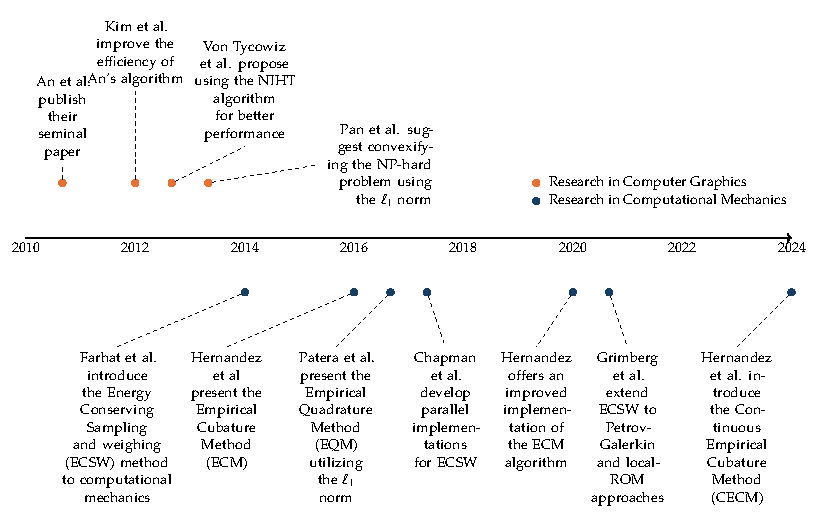
\includegraphics[width=\linewidth]{PAT.pdf}
\caption{A brief history of cubature rules/mesh sampling procedures \cite{an2009optimizing,kim2013subspace,von2013efficient,pan2015subspace,farhat2014dimensional,chapman2016accelerated,Patera_2017_EQP,hernandez2020multiscale,grimberg2021mesh,hernandez2024cecm}. Adapted from \cite{bravo2024subspace}.}
\label{fig:PTA_LIT}
\end{figure}


\subsubsection*{Determining $\boldsymbol{\xi}$}

We begin by utilizing the available high-fidelity solution snapshots obtained for different parameter values to determine the corresponding reduced balance vectors $\vec{b}_n$.
For a time-dependent problem, consider a solution snapshot $\vec{w}_n$ for the $k^{\text{th}}$ parameter pair ($\boldsymbol\mu_k$, $t_k$).
We write from \cref{eq:r_n}

\begin{align}
\vec{b}^{k}_n(\vec{w}_n(\mu_k, t_k); \mu_k) = \sum_{e=1}^{n_{\text{cell}}} \boldsymbol{\gamma}^{k,e}_{n},
\label{eq:bn_sum}
\end{align}

where $\vec{b}^{k}_n$ is the balance vector for the $k^{\text{th}}$ parameter and $\boldsymbol{\gamma}^{k,e}_{n} = \mathbb{W}_e^{\top} \vec{b}_e (\mathcal{Q}_e\vec{w}^{ref} + \widetilde{\mathbb{U}}_e \vec{w}_n(\mu_k, t_k); \mu_k)$.
Note that here time $t$ is considered as a parameter as well.
For different parameters the choice of the time-points need not be same.
They are  chosen based on the nature of the solution.


At the offline stage, $\vec{w}_n(\mu_k, t_k)$ is calculated by projecting the $N$-dimensional high-fidelity solution snapshot $\vec{w}_N(\mu_k, t_k)$ onto the reduced basis $\widetilde{\mathbb{U}}$, and is \textit{not} the solution to a reduced order model:

\begin{equation}
\vec{w}_n(\mu_k, t_k) = \widetilde{\mathbb{U}}^{\top} \left(\vec{w}_N(\mu_k, t_k)-\vec{w}^{ref}\right).    
\end{equation}

We rewrite \cref{eq:bn_sum} as:

\begin{equation}
\vec{b}_n^{k} = \bar{\mat{G}}^{k}\, \vec{1},
\label{eq:bn_G1}
\end{equation}

where $\bar{\mat{G}}^k \in \mathbb{R}^{n \times n_{\text{cell}}}$ and $\vec{1} \in \mathbb{R}^{n_{\text{cell}} \times 1}$ are defined as:

\begin{subequations}
\begin{equation}
\bar{\mat{G}}^k = \left[ \boldsymbol{\gamma}_n^{k,1},\ \boldsymbol{\gamma}_n^{k,2},\ \dots,\ \boldsymbol{\gamma}_n^{k,n_{\text{cell}}} \right],
\end{equation}
\begin{equation}
\vec{1} = \left[ 1,\ 1,\ \dots,\ 1 \right]^{\top}.
\end{equation}
\end{subequations}

If $N_s$ solution snapshots are generated for $N_s$ pairs of $\mu$ and $t$, \cref{eq:bn_G1} can be extended to:

\begin{equation}
\boldsymbol{\Gamma} = \mat{G}\, \vec{1},
\label{eq:Gamma_G1}
\end{equation}

where $\mat{G} \in \mathbb{R}^{n N_s \times n_{\text{cell}}}$ (typically $n N_s < n_{\text{cell}}$) and $\boldsymbol{\Gamma} \in \mathbb{R}^{n N_s \times 1}$ are defined as:

\begin{subequations}
\begin{equation}
\boldsymbol{\Gamma} = \left[ \vec{b}_n^{1\,\top}, \vec{b}_n^{2\,\top}, \hdots, \vec{b}_n^{N_s\,\top}\right]^\top,
\end{equation}
\begin{equation}
\mat{G} = \left[ \bar{\mat{G}}^{1\,\top}, \bar{\mat{G}}^{2\,\top}, \hdots, \bar{\mat{G}}^{N_s\,\top}\right]^\top.
\end{equation}
\end{subequations}


Our goal is to replace the vector $\vec{1}$ in \cref{eq:Gamma_G1}, which assigns equal weight to the elemental contributions, with a sparse weighing vector $\boldsymbol{\xi}$ such that:
\begin{equation}
\boldsymbol{\Gamma} \approx \mat{G}\, \boldsymbol{\xi},
\label{eq:Gamma_Gxi}
\end{equation}
implying:
\begin{align}
\vec{b}^k_n \approx \sum_{e=1}^{n_{\text{cell}}} \xi_e\, \boldsymbol{\gamma}^{k,e}_{n}
\label{eq:bn_approx}
\end{align}

To obtain a sparse $\boldsymbol{\xi}$, we ideally want to minimize its zero norm (the number of non-zero elements):

\begin{equation}
\boldsymbol{\xi}^\ast = \arg \min_{\boldsymbol{\xi} \in \mathbb{R}^{n_{\text{cell}}},\ \boldsymbol{\xi} \geq 0} \| \boldsymbol{\xi} \|_0 \quad \text{subject to} \quad \| \mat{G}\, \boldsymbol{\xi} - \boldsymbol{\Gamma} \|_2 \leq \epsilon \| \boldsymbol{\Gamma} \|_2.
\label{eq:L0_min}
\end{equation}

where $\epsilon$ is some pre-defined tolerance.
However, this problem is NP-hard \cite{farhat2014dimensional}.
Therefore, we use approximations such as non-negative $L_1$-norm minimization, non-negative $L_2$-norm minimization with $L_1$-norm regularization, or non-negative least squares (NNLS).

Among these, NNLS \cite{NNLSLawsonHanson1995} is most commonly employed for ECSW.
NNLS solves the linear least squares problem under the constraint that the solution must be non-negative:

\begin{equation}
\boldsymbol{\xi}^\ast = \arg \min_{\boldsymbol{\xi} \in \mathbb{R}^{n_{\text{cell}}},\ \boldsymbol{\xi} \geq 0} \| \mat{G}\, \boldsymbol{\xi} - \boldsymbol{\Gamma} \|_2^2.
\label{eq:NNLS}
\end{equation}

While NNLS does not explicitly promote sparsity, it often results in a sparse $\boldsymbol{\xi}$ in practice, providing an acceptable approximation of $\boldsymbol{\Gamma}$ with a non-negative and sparse solution.
\vspace{-10pt}
\remark
 An effective approach to speed up NNLS computations in \cref{eq:NNLS} is by parallelizing the NNLS algorithm via domain decomposition, thereby distributing the workload among multiple processors.
This method involves dividing the finite element (FE) mesh into subdomains, effectively partitioning the matrix $\mat{G}$ column-wise.
By computing $\boldsymbol{\Gamma}$ for each column partition and employing the NNLS solver on each subdomain independently, this technique minimizes offline computation costs.
\vspace{-8pt}
\remark We observed that the NNLS computations can be made further efficient by using a low-rank approximation of $\mat{G}$ through its SVD.
By decomposing \(\mat{G} = \mat{U}_r \mat{\Sigma}_r \mat{V}_r^\top\), where \(\mat{U}_r\), \(\mat{\Sigma}_r\), and \(\mat{V}_r\) correspond to the top \(r\) singular values, we can transform the objective function in \cref{eq:NNLS} into \(\|\mat{V}_r^\top \boldsymbol{\zeta} - \mathbf{d}_r\|_2^2\), where \(\mathbf{d}_r = \mat{V}_r^\top \cdot \mathbf{1}\).
This transformation to the reduced space improves computational efficiency.
Most importantly it helps eliminate redundancy in the snapshots data.
\vspace{-8pt}
\remark Parallel implementations of NNLS in \texttt{C++} can be found in libraries such as \texttt{libROM}\footnote{\texttt{libROM}: A library for reduced-order modeling, available at \url{https://github.com/LLNL/libROM}}.
Such implementations are suitable for handling large-scale problems by utilizing parallel computing architectures.
\vspace{-19pt}
\remark Energy-Conserving Sampling and weighing (ECSW) preserves the Lagrangian structure crucial for second-order hyperbolic problems governed by Hamilton's principle.
This preservation ensures that time integrators unconditionally stable for Parametrically Reduced-Order Models (PROMs) remain stable when applied to the hyper-ROMs produced by ECSW.
\vspace{-8pt}
\remark ECSW demonstrates superior numerical stability and accuracy in structural dynamics problems where other hyper-reduction methods, particularly those using the approximate-then-project approach, often fail—making it especially valuable for applications requiring robust numerical performance.



\subsubsection*{Implementation on the running example}
As before, we use the same training and test datasets—each consisting of 16 parameter pairs \((\mu, \beta)_k\) for \(k=1, \ldots, 16\)—to formulate and evaluate the ECSW-based hyper-reduced order models (hyper-ROMs).
Here, \(\widetilde{\mathbb{U}}\) remains identical to the matrix employed for the regular ROM discussed in Section \ref{sec:ROM_example}, with \(n=5\) columns.


In the offline phase, to compute a reduced mesh, we construct the matrix $\mat{G}$ by incorporating element-level contributions $\boldsymbol{\gamma}^{k,e}_n$ from various solution snapshots as in \cref{eq:bn_sum}. 
For the $e$-th element, we define the projected elemental stiffness matrix as
\begin{equation}
    \mat{K}^{k,e}_n = \widetilde{\mathbb{U}}_e^{\top} \mat{K}^{k}_e \widetilde{\mathbb{U}}_e,
\end{equation}
the projected temperature vector as
\begin{equation}
    \widetilde{\vec{T}}^k_n = \widetilde{\mathbb{U}}^{\top} \left( \overline{\vec{T}} +  \widetilde{\mathbb{U}}\widetilde{\mathbb{U}}^{\top}\left(\vec{T}^{k}_N - \overline{\vec{T}}\right) \right),
    \label{eq:red_snapshot}
\end{equation}
and the projected source vector as
\begin{equation}
    \vec{f}^{k,e}_n = \widetilde{\mathbb{U}}_e^{\top} \vec{q}_e(\beta_k),
\end{equation}
for the $k$-th solution snapshot.
The element-level balance vector is then written as
\begin{equation}
    \boldsymbol{\gamma}^{k,e}_{n} = \mat{K}^{k,e}_n \,\widetilde{\vec{T}}^k_n - \vec{f}^{k,e}_n.
    \label{eq:gamma_n_exampleP}
\end{equation}


Using these snapshots alongside Equations \eqref{eq:bn_sum} to \eqref{eq:NNLS}, we determine the sparse elemental weight vector $\boldsymbol{\xi}$.
This process results in the selection of only 11 elements out of the 5000 in the domain, as depicted in \cref{fig:reduced_mesh_ecsw}.
The value of the objective function \cref{eq:NNLS} is approximately $10^{-9}$, indicating a successful minimization.
This remarkable reduction in the number of mesh elements obviates the need to evaluate 5000 elemental stiffness matrices during every Newton-Raphson iteration.


In \cref{fig:stiffness_matrices}, we provide a visual representation of how ECSW reduces the computational cost of evaluating the reduced nonlinear stiffness matrix.
\Cref{fig:visual_FOM_FEA_2} depicts the derivation of the reduced stiffness matrix where elemental contributions are equally weighted.
In contrast, \cref{fig:visual_ROM_FEA} shows an approximate reduced stiffness in which the stiffness matrix at the bottom has a non-zero and non-unit weight of $w_i$, and the weight of the top element is zero.
The resulting reduced stiffness matrix looks approximately similar to the actual reduced stiffness matrix; however, the cost associated with evaluating the top stiffness matrix is eliminated.



In \cref{fig:HROM_ERROR_SPDUP}, the relative percentage error (Eq.~\ref{eq:rom_error}) and speed-up (Eq.~\ref{eq:rom_speedup}) of the hyper-ROM are compared with those of the regular projection-based ROM.
\Cref{fig:HROM_ERROR_SPDUP_a} demonstrates that the hyper-ROM achieves high accuracy, with a relative error of approximately 0.0001\%.
While this error is marginally higher than that of the ROM, the computational speed-up is remarkable—nearly $300\times$ the speed-up of the regular ROM.
This performance gain is almost an order of magnitude greater than the speed-up achieved through DEIM.
We attribute this additional improvement to the high accuracy with which ECSW approximates the reduced quantities, which presumably results in a  faster Newton iteration convergence compared to DEIM.


\begin{figure}[t]
    \centering
    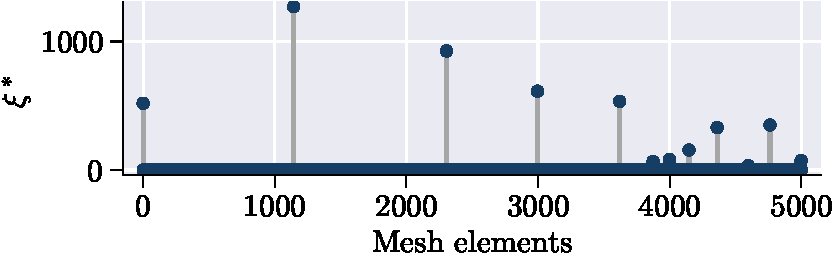
\includegraphics[width=0.8\linewidth]{reduced_mesh_ECSW_new.pdf}
    \caption{Stem plot illustrating the reduced mesh obtained via ECSW-based hyper-reduction. The plot highlights the mesh elements with non-zero weights $\xi^*$ (Eq.~\ref{eq:NNLS}). The weights for all elements lying on the blue line are zero. The reduced mesh comprises only 11 elements, which constitutes 0.2\% of the total 5,000 elements in the original mesh.}
    \label{fig:reduced_mesh_ecsw}
\end{figure}


\begin{figure}[t]
    \centering
    \begin{subfigure}{0.48\linewidth}
        \hspace{-15pt}
        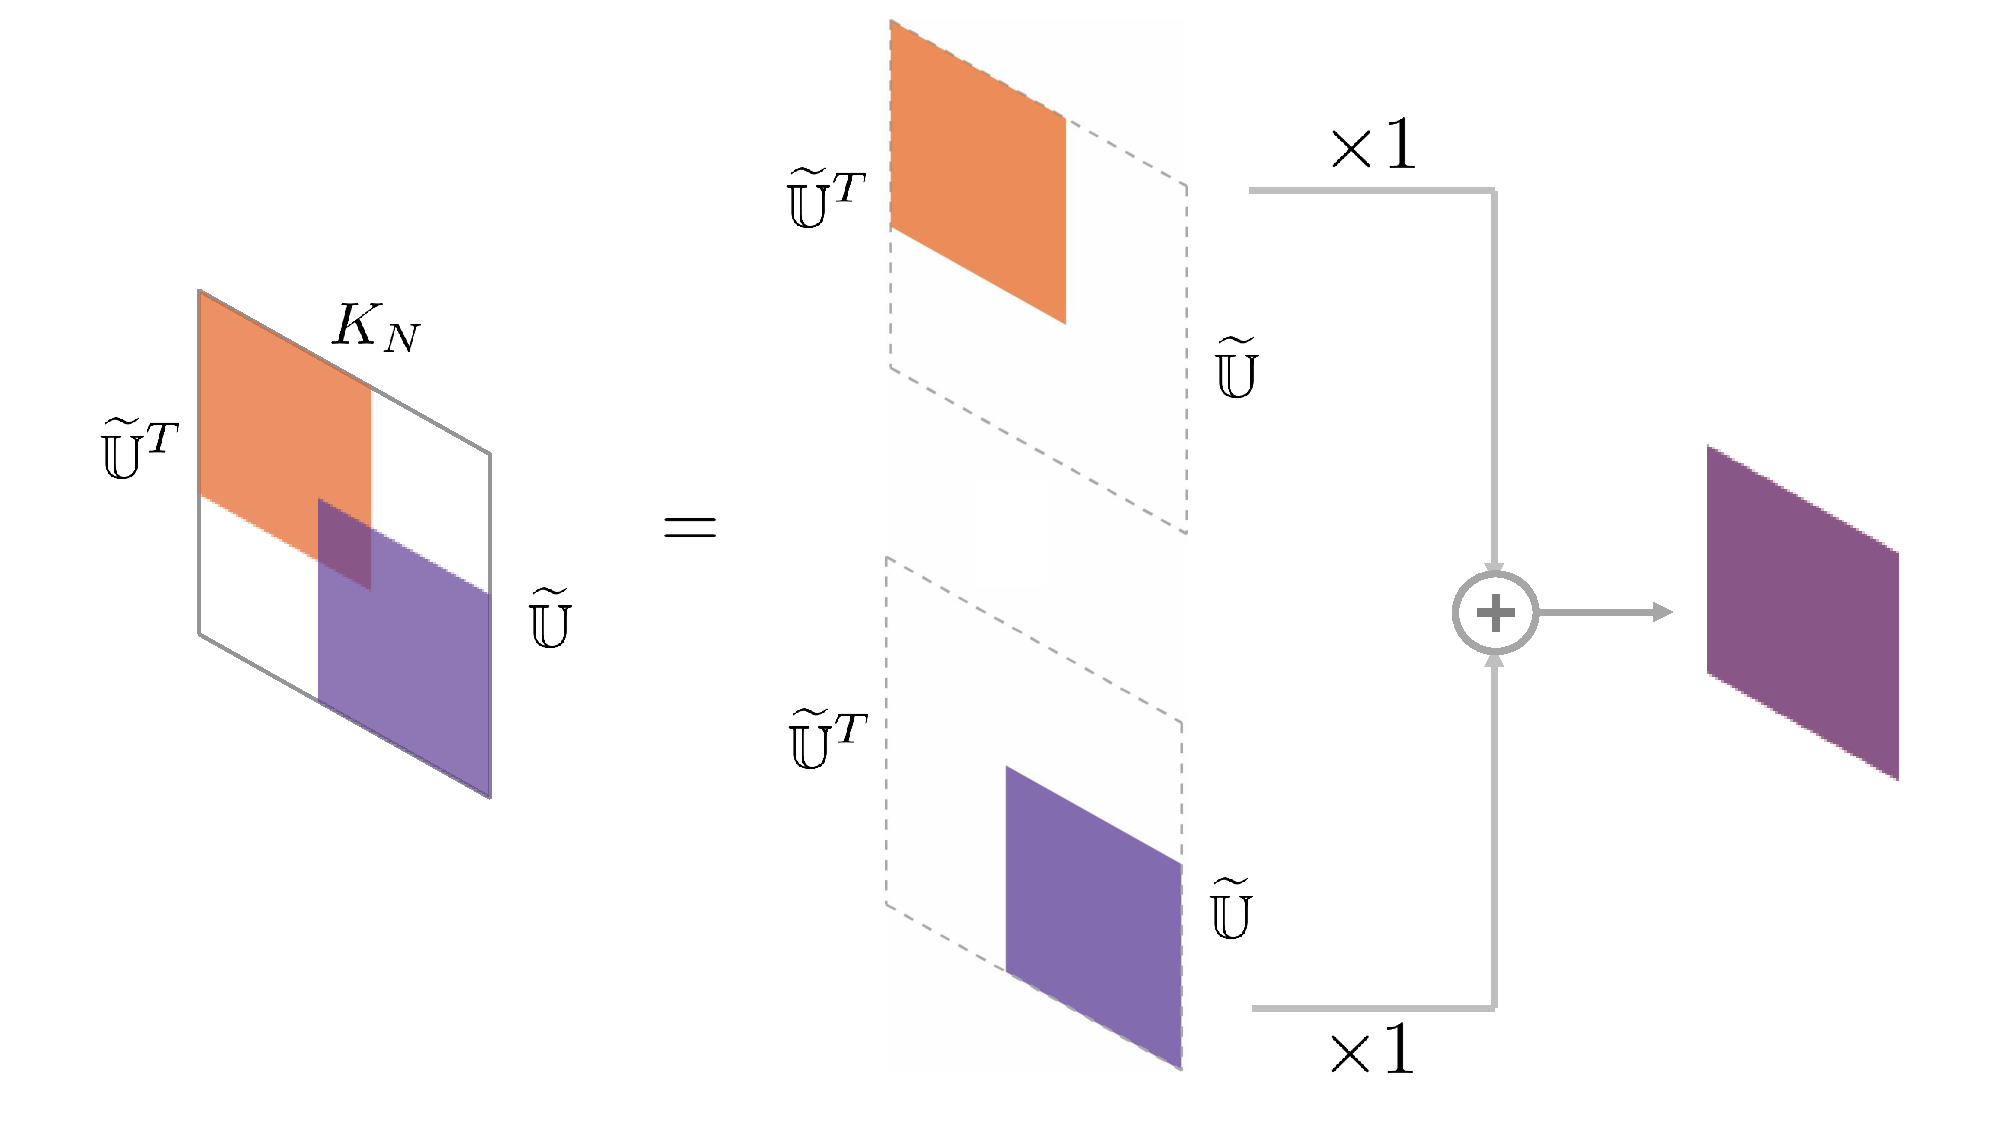
\includegraphics[width=\linewidth]{K_red.pdf}
        \caption{}
        \label{fig:visual_FOM_FEA_2}
    \end{subfigure}%
\begin{subfigure}{0.48\linewidth}
        \centering
        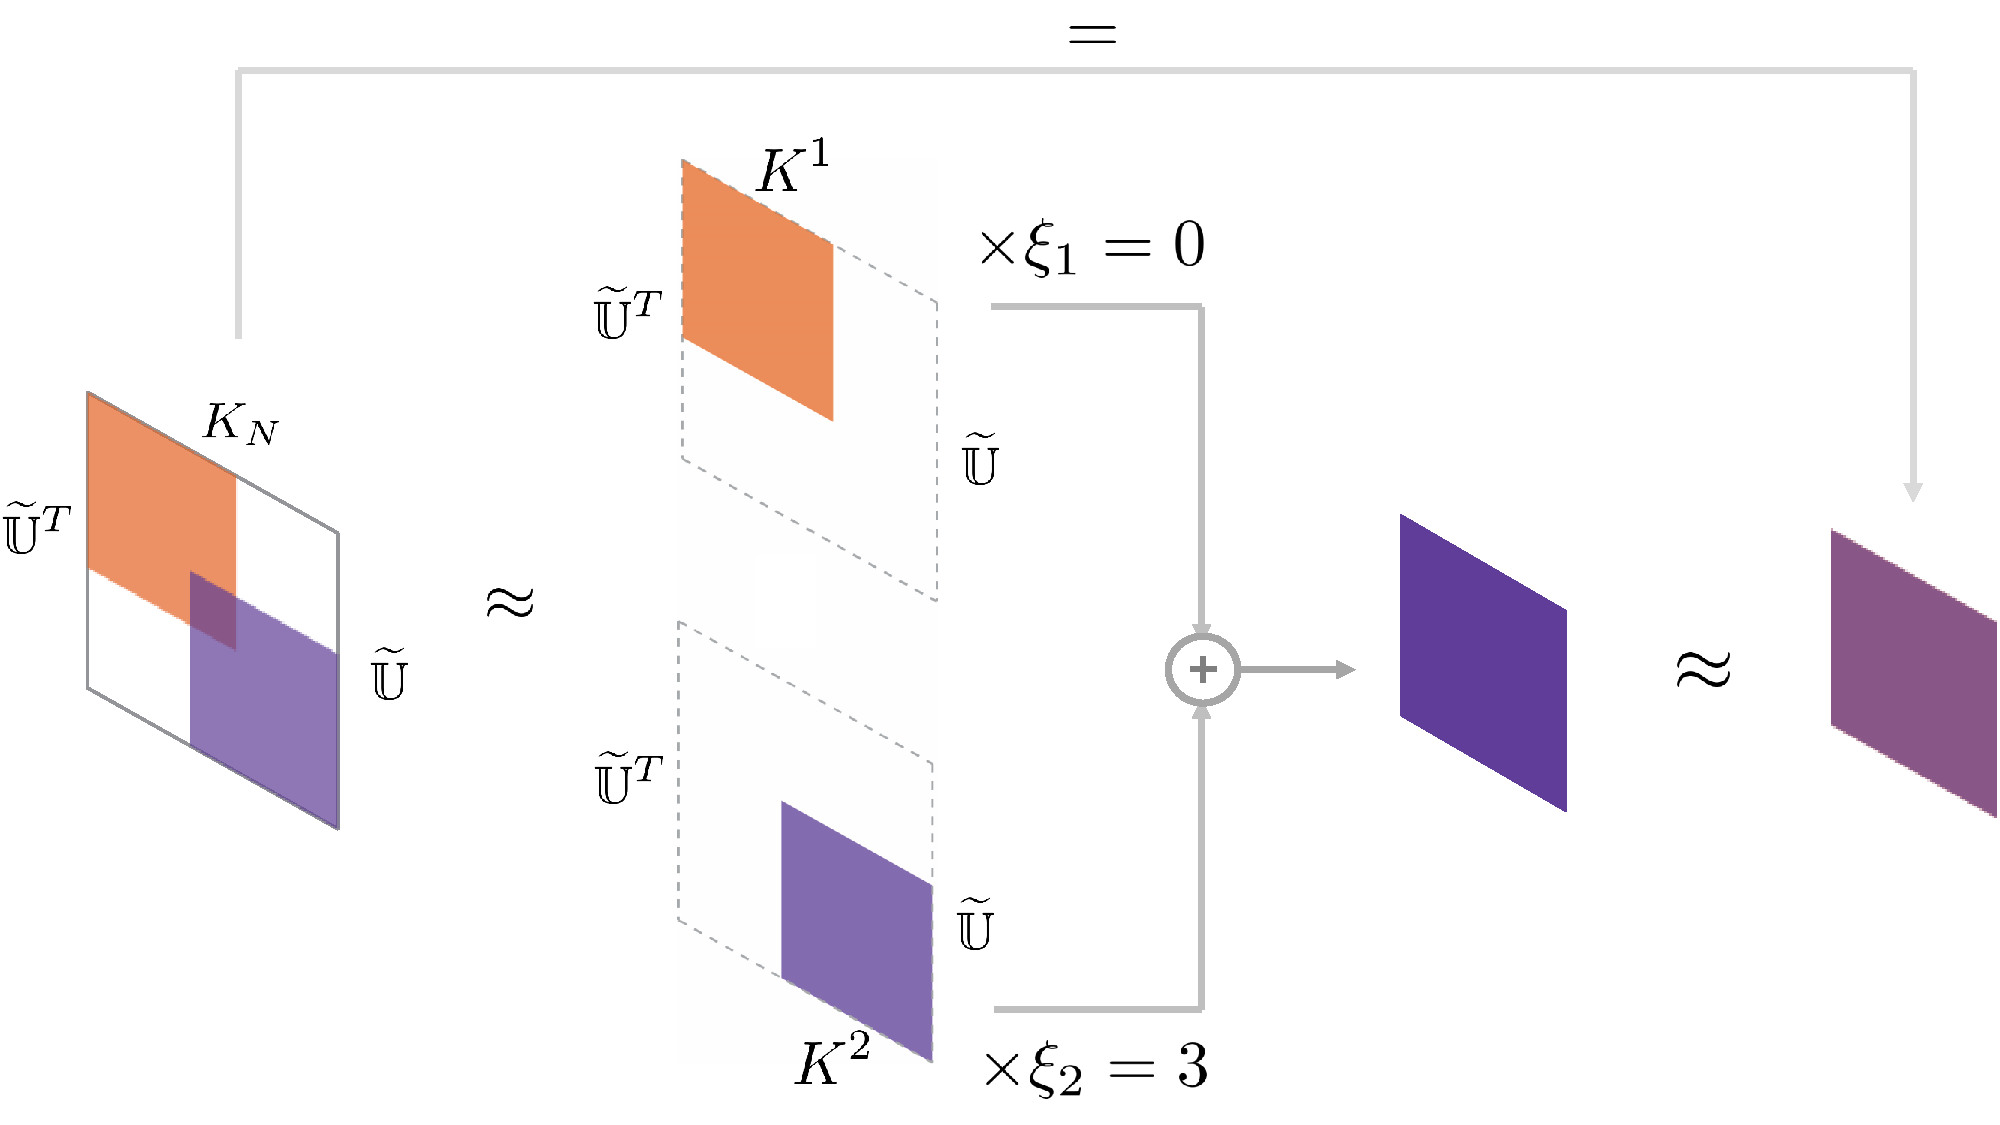
\includegraphics[width=\linewidth]{K_hyper_red.pdf}
        \caption{}
        \label{fig:visual_ROM_FEA}
    \end{subfigure}
\caption{Reduction in the computational cost of evaluating the reduced nonlinear stiffness matrix achieved with ECSW during the iterative solution process. (a) Derivation of the reduced stiffness matrix with equally weighted elemental contributions without hyper-reduction. (b) Efficient \textit{approximation} of the reduced stiffness matrix where the top element's weight \(\xi_1\) is zero, and the bottom element has a much larger weight \(\xi_2\), eliminating the cost of evaluating the top stiffness matrix during solution iteration.}
\label{fig:stiffness_matrices}
\end{figure}

\begin{figure}[t]
\centering
\begin{subfigure}[b]{0.47\linewidth}
\centering
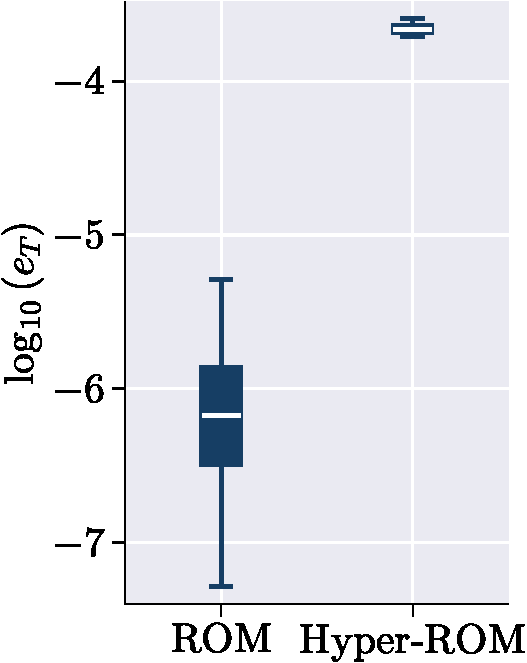
\includegraphics[height=0.95\linewidth]{error_comp_rom_hrom_ecsw.pdf}
\caption{}
\label{fig:HROM_ERROR_SPDUP_a}
\end{subfigure}\hfill
\begin{subfigure}[b]{0.47\linewidth}
\centering
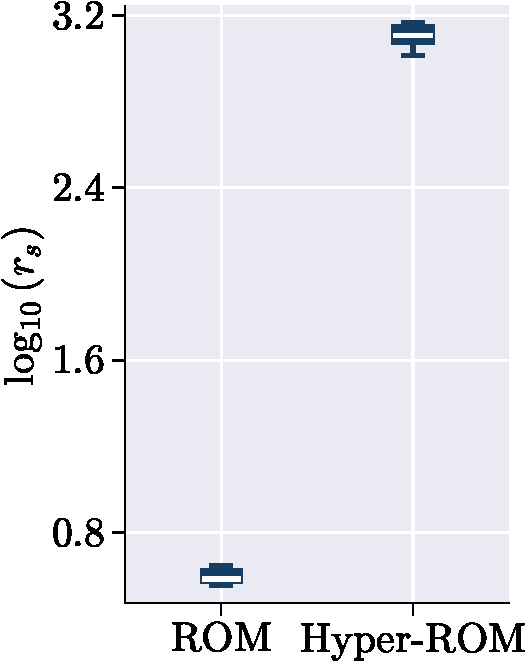
\includegraphics[height=0.95\linewidth]{speed_up_comp_rom_hrom_ecsw.pdf}
\caption{}
\label{fig:HROM_ERROR_SPDUP_b}
\end{subfigure}
\caption{Difference in accuracy ($e_T$) and speed-up ($r_s$) between the regular projection based ROM and ECSW Hyper-ROM.}
\label{fig:HROM_ERROR_SPDUP}
\end{figure}


\remark The Non-Negative Least Squares (NNLS) algorithm can be implemented in Python using the \texttt{scipy.optimize.nnls} function \cite{2020SciPy-NMeth}.
However, the standard version may be inefficient for large-scale problems.
\vspace{-8pt}
\remark Starting from SciPy version 1.13.1, the \texttt{nnls} function was improved by integrating the fast Non-Negativity-Constrained Least Squares (fast-NNLS \cite{fastnnls1997}) algorithm.
This method uses an active set approach for faster convergence, particularly benefiting large-scale applications.
The updated function also allows users to adjust error tolerance via the \texttt{atol} parameter.
\vspace{-8pt}

\remark Here we implemented the \texttt{fast-NNLS} algorithm from \texttt{scipy 1.13.1} with a tolerance of $10^{-4}$.

\remark While performing NNLS, it is important to check that the magnitude of $\Gamma$ in Equation \eqref{eq:NNLS} is at least a few orders of magnitude larger than the tolerance.
A small $\Gamma$ often leads to a dense weight vector $\boldsymbol{\xi}$ instead of sparse.








\subsubsection{Empirical cubature method (ECM)}




\noindent\hrulefill
\begin{itemize}
    \item \textbf{Objective:} Devise efficient cubature rules for the integrals in the reduced governing equations, typically resulting from the inner product with reduction bases.
    \item Low-dimensional solution structures imply low-dimensionality of nonlinear integrands.
    \item The integrals can be computed more efficiently using far fewer cubature points than high-fidelity models require.
    \item Compute projection integrals by evaluating the integrand over all cubature points for multiple parameter instances and express the exact integrals as a matrix-vector product.
    \item Formulate the matrix for element contributions and gather all Gauss weights into a single vector.
    \item Identify a subset of points and adjust the associated weights to approximate the vector of exact integrals with desired accuracy.
\end{itemize}
\noindent\hrulefill


The Empirical Cubature Method (ECM) \cite{hernandez2017dimensional} focuses on efficiently approximating the integrals of a system's internal forces, which are essential for computing system matrices in approaches like the Finite Element Method.
The key idea is that internal forces, similar to high-fidelity solutions, reside in a low-dimensional subspace that is independent of the finite element mesh size.
This characteristic allows their integrals to be efficiently approximated using a cubature rule with significantly fewer points than those used in standard methods.


\subsubsection*{Problem formulation}
The Empirical Cubature Method (ECM) identifies cubature points using a limited set of high-fidelity training data, as seen in other methods.
To illustrate the approach, we first outline its application for a general \( n \)-dimensional parameterized vector-valued function \( \vec{a} \), and subsequently demonstrate its use in hyper-reduced order models.
This section is adapted from \cite{hernandez2024cecm}, and follows the notation presented therein.


Let us define the vector-valued function \(\vec{a}: \Omega \times \mathcal{P} \to \mathbb{R}^n\), where \(\Omega\) is the spatial domain partitioned into finite elements as \(\Omega = \bigcup_{e=1}^{N_e} \Omega^e \subset \mathbb{R}^d\) with \(d = 1, 2,\) or \(3\), and \(\mathcal{P}\) is the parameter domain.
All finite elements \(\Omega^e\) are assumed to be isoparametric and share the same interpolation order, each containing \(r\) Gauss integration points.
For a set of \(N_s\) parameter instances \(\{ \mu_j \}_{j=1}^{N_s} \subset \mathcal{P}\), and given the values of the integrand at all Gauss points, the integral of the function over \(\Omega\) for each parameter \(\mu_j\) is computed using the element-wise Gauss quadrature rule:


\begin{equation}
b_k = \sum_{e=1}^{n_{\text{cell}}} \int_{\Omega^e} a_i(x, \mu_j) \, d\Omega = \sum_{e=1}^{n_{\text{cell}}} \sum_{g=1}^{r} a_i(x_g^e, \mu_j) W_g^e, \quad \text{where} \quad k = (j-1)n + i,
\end{equation}


for \(j = 1, \ldots, N_s\) and \(i = 1, \ldots, n\).
In this equation, \(x_g^e \in \Omega^e\) denotes the position of the \(g\)-th Gauss point within element \(\Omega^e\), and \(W_g^e > 0\) is the weight associated with the \(g\)-th Gauss point, calculated as the product of the Gauss weight and the Jacobian determinant for the isoparametric transformation.
The quantity \(b_k\) represents the "exact" integral value for each component \(i\) of \(\vec{a}\) and parameter instance \(\mu_j\), serving as the reference value we aim to approximate.
Here, \(n_{\text{cell}}\) denotes the total number of finite elements.

This computation can be concisely expressed in matrix form:
\begin{equation}
\mathbf{b}_{\text{FE}} = \mat{A}_{\text{FE}}^\top \mathbf{W}_{\text{FE}},
\end{equation}
where \(\mathbf{b}_{\text{FE}} \in \mathbb{R}^{nN_s}\) is the vector of "exact" integrals for all components and parameter instances.
The matrix \(\mat{A}_{\text{FE}}\) contains the values of the integrand \(a_i(x_g^e, \mu_j)\) at all Gauss points for each parameter \(\mu_j\), and \(\mathbf{W}_{\text{FE}}\) is a column vector containing all the finite element weights \(W_g^e\).
The ECM matrix $\mat{A}_{FE}\in\mathcal{R}^{M\times n N_s}$ ($M = r n_{cell}$ is the total number of original cubature points) can be expressed in terms of element contributions as:
\begin{equation}
\mat{A}_{FE} = \left[ 
\mat{A}_{FE}^{(1)\,\top}, 
\mat{A}_{FE}^{(2)\,\top},\quad
\hdots\quad
,\mat{A}_{FE}^{(n_{\text{cell}})\,\top} 
\right]^\top
\end{equation}
where each block matrix \(\mat{A}_{FE}^{(e)} \in \mathbb{R}^{r \times nN_s}\) corresponds to the \(r\) Gauss points of element \(e\) and is defined as:
\begin{equation}
\mat{A}_{FE}^{(e)} = 
\begin{bmatrix} 
a_1(x_1^e, \mu_1) & a_2(x_1^e, \mu_1) & \cdots & a_n(x_1^e, \mu_1) & a_1(x_1^e, \mu_2) & \cdots & a_n(x_1^e, \mu_{N_s})\\ 
a_1(x_2^e, \mu_1) & a_2(x_2^e, \mu_1) & \cdots & a_n(x_2^e, \mu_1) & a_1(x_2^e, \mu_2) & \cdots & a_n(x_2^e, \mu_{N_s})\\ 
\vdots & \vdots & \ddots & \vdots & \vdots & \ddots & \vdots \\ 
a_1(x_r^e, \mu_1) & a_2(x_r^e, \mu_1) & \cdots & a_n(x_r^e, \mu_1) & a_1(x_r^e, \mu_2)  & \cdots & a_n(x_r^e, \mu_{N_s}) 
\end{bmatrix}
\end{equation}


Similarly, the vector of quadrature weights \(\mathbf{W}_{FE} \in \mathbb{R}^{M \times 1}\) is expressed as:
\begin{equation}
\mathbf{W}_{FE} = \left[\vec{W}_{FE}^{(1)\top},
\vec{W}_{FE}^{(2)\top},\quad
\hdots\quad
,\vec{W}_{FE}^{(n_{\text{cell}})\top}\right]^\top
\label{eq:gaussian_weights}
\end{equation}
where each sub-vector \(\vec{W}_{FE}^{(e)} \in \mathbb{R}^{r \times 1}\) contains the weights for the Gauss points of element \(e\):
\begin{equation}
\vec{W}_{FE}^{(e)} = \left[ W_1^e, W_2^e, \quad\hdots\quad, W_r^e \right]^\top
\end{equation}
This formulation organizes the integrand values and corresponding weights for each finite element and Gauss point.

We further define vector $\vec{X}_{FE}\in\mathcal{R}^{M\times 1}$ which contains  the corresponding cubature points:
\begin{equation}
\mathbf{X}_{FE} = \left[\vec{X}_{FE}^{(1)\top}, 
\vec{X}_{FE}^{(2)\top},\quad
\hdots\quad
,\vec{X}_{FE}^{(n_{\text{cell}})\top}\right]^\top
\label{eq:X_points}
\end{equation}
and
\begin{equation}
\vec{X}_{FE}^{(e)} = \left[ x_1^e, x_2^e, \quad\hdots\quad, x_r^e \right]^\top
\end{equation}





\subsection*{Finding cubature points}
Similar to ECSW, we aim to find a sparse set of cubature points \( X = \{ x_g \}_{g=1}^{m} \) with \( x_g \in \Omega \) and their associated positive weights \( \{ \omega_g \}_{g=1}^{m} \), where \( m \ll M \).
The objective is to minimize \( m \) while approximating the vector of "exact" integrals \( \mathbf{b}_{FE} \) to a desired accuracy \( 0 \leq \epsilon \leq 1 \) by solving this best subset selection optimization problem:










\begin{equation}
\min_{\boldsymbol{\omega} \geq 0} \| \boldsymbol{\omega} \|_0, \quad \text{subject to} \quad \left\| \mat{A}_{FE}^\top \boldsymbol{\omega} - \mat{A}_{FE}^\top \vec{W}_{FE} \right\|_2 \leq \epsilon_b \left\| \mat{A}_{FE}^\top \vec{W}_{FE} \right\|_2,
\label{eq:ecm_opt2}
\end{equation}

where $\boldsymbol{\omega}\in\mathcal{R}^{M\times 1}$ \(\| \boldsymbol{\omega} \|_0\) denotes the \(l_0\)-norm, counting the number of nonzero entries in \(\boldsymbol{\omega}\), which we denote using $m$, and \(\epsilon_b\) is a specified tolerance.
However, as discussed in \cref{sec:ECSW}, such sparsity-promoting optimization problems are NP-hard and are typically solved using suboptimal greedy heuristics or convex relaxation techniques, such as non-negative least squares \cite{NNLSLawsonHanson1995,fastnnls1997} and non-negative \(l_1\)-norm minimization \cite{Patera_2017_EQP}.


However, the newly developed cubature point selection algorithm (see \cref{alg:ECM_PS}) introduced in \cite{bravo2024subspace} offers an efficient and optimal \textit{sparse} solution for the following alternative linear-least square problem:

\begin{equation}
\boldsymbol{\omega} = \arg \min_{\boldsymbol{\omega^*} \in \mathbb{R}^{M\times 1},\ \boldsymbol{\omega^*} \geq 0} \quad \left\| \mat{A}_{FE}^\top \boldsymbol{\omega^*} - \mat{A}_{FE}^\top \vec{W}_{FE} \right\|_2 
\label{eq:alternative_min_ecm}
\end{equation}




The python and MATLAB implementations of the algorithm is available at  Ref.~\cite{ecm_python_GitHub}.


\subsection*{Dimension reduction of $\mat{A}_{FE}$}

To reduce the computational cost of solving \cref{eq:alternative_min_ecm}, we approximate and decompose the ECM matrix \(\mat{A}_{FE}\) using singular value decomposition (SVD):
\begin{equation}
\mat{A}_{FE} \approx \widetilde{\mathbb{W}}\, \mat{S}\, \underline{\mathbb{V}}^{\top},
\end{equation}
where \(\widetilde{\mathbb{W}} \in \mathbb{R}^{M \times m}\) contains the left singular vectors for the \(m\) retained modes, \(\mat{S} \in \mathbb{R}^{m \times m}\) is the diagonal matrix of singular values, and \(\underline{\mathbb{V}} \in \mathbb{R}^{nN_s \times m}\) contains the corresponding right singular vectors.



As a result of this reduction, the objective function in \cref{eq:alternative_min_ecm} transforms into:
\begin{equation}
\left\| \mat{V} \mat{\Sigma} \left( \widetilde{\mathbb{W}}^{\top} \boldsymbol{\omega} - \widetilde{\mathbb{W}}^{\top} \vec{W}_{FE} \right) \right\|_2.
\label{eq:ecm_opt2_a}
\end{equation}
This reformulation simplifies the optimization problem, making it  computationally more tractable. 
We then use the cubature point selection strategy described in \cref{alg:ECM_PS} to solve this approximate optimization problem, which essentially boils down to finding  a sparse $\boldsymbol{\omega}$ such that
\begin{equation}
\widetilde{\mathbb{W}}^{\top} \boldsymbol{\omega} \approx \widetilde{\mathbb{W}}^{\top} \vec{W}_{FE}
\label{eq:ecm_opt3}
\end{equation}
The algorithm essentially yields $\boldsymbol{\omega}$ and a selection matrix $\mat{P}_z\in \mathcal{R}^{m\times M}$ with each row containing a single non-zero entry at the index specified by $z$ such that
\begin{equation}
\mat{P}_z \mathbb{\widetilde{W}} =
\begin{bmatrix}
w_1(x_1^*) & w_2(x_1^*) & \cdots & w_p(x_1^*) \\
w_1(x_2^*) & w_2(x_2^*) & \cdots & w_p(x_2^*) \\
\vdots & \vdots & \ddots & \vdots \\
w_1(x_m^*) & w_2(x_m^*) & \cdots & w_p(x_m^*)
\end{bmatrix}_{m \times m}
\end{equation}
where  
\begin{equation}
\mat{P}_z \vec{X}_{FE} = X^* = [x_1^*, x_2^*, \ldots, x_m^*]^{\top}
\end{equation}
are the cubature points corresponding to nonzero entries of $\boldsymbol\omega$. 
In essence,
\begin{equation}
(\mat{P}_z\widetilde{\mathbb{W}})^{\top} \mat{P}_z\boldsymbol{\omega} = \widetilde{\mathbb{W}}^{\top} \boldsymbol\omega
\end{equation}
This sparse selection of the cubature points leads to a reduced mesh, which is then used to compute the parametric nonlinearity more efficiently.




\subsection*{Implementation on the running example}
To implement ECM on the example problem in \cref{sec:ROM_example}, we begin by writing the nonlinear reduced stiffness matrix and the force vector in terms of the gauss-quadrature points for the $j-$th parameter pair $(\mu_j,\beta_j)$:

\begin{equation}
	\mat{K}_n(\mathbf{T}_n; \mu)  = \sum_{e=1}^{n_{\text{cell}}} \mat{K}^e_n,
	\label{eq:elemental_contrib_K_red}
\end{equation}
where
\begin{equation}
\mat{K}_n^e = \sum_{g=1}^{r}\,\,w_g\,\, \mat{K}_n^e(\vec{x}^e_g)
\end{equation}
and
\begin{equation}
\mathsf{K}_n^e(\vec{x}^e_g) =  k({T}(\vec{x}^{e}_{g};\mu_j,\beta_j),\mu_j)\,\widetilde{\mathbb{U}}^{e\,\top}{\nabla \boldsymbol\Phi}^e(\vec{x}^{e}_g) {\nabla\boldsymbol\Phi}^e(\vec{x}^{e}_g)^\top\widetilde{\mathbb{U}}^e  
\label{eq:elemental_stiffness_matrix}
\end{equation}
Here $k({T}(\vec{x}^{e}_{g};\mu_j,\beta_j);\mu_j)$ is the nonlinear thermal conductivity evaluated at $\vec{x}^e_g$, where $\vec{x}^{e}_g\in \Omega^e$ is the $g$-th cubature point within the $e-$th cell; $w^{e}_g$ is the cubature weight associated with $\vec{x}^{e}_g$; vector $\boldsymbol\Phi^e(\vec{x}^{e}_g) = [\phi^{e}_1(\vec{x}^{e}_g),\phi^{e}_2(\vec{x}^{e}_g)]^\top$ contains the two Lagrange basis functions associated with element $e$, which were used in the high fidelity finite element model in \cref{eq:FE_shape}; and $\widetilde{\mathbb{U}}^e$ is as defined in \cref{eq:ue_we}.


Similarly, the nonlinear reduced force vector is given by

\begin{equation}
	\vec{f}_n(\mathbf{T}_n; \mu) = \sum_{e=1}^{n_{\text{cell}}} \vec{f}^e_n,
	\label{eq:elemental_contrib_f_red}
\end{equation}
where
\begin{equation}
	\vec{f}^e_n = \sum_{g=1}^{r} \,\, w_g \,\, \vec{q}^e(\vec{x}^e_g),
	\label{eq:elemental_force_vector}
\end{equation}
and
\begin{equation}
\vec{q}_n^e(\vec{x}^e_g) = q(T(\vec{x}^{e}_{g}; \mu_j, \beta_j),\beta_j) \widetilde{\mathbb{U}}^{e\,\top} \, \boldsymbol\Phi^{e}(\vec{x}^{e}_g),
\label{eq:source_term_expression}
\end{equation}
where \( q({T}(\vec{x}^{e}_{g};\mu_j,\beta_j);\beta_j) \) represents the nonlinear source term evaluated at $\vec{x}^e_g\in\Omega^e$.


In ECM, similar to ECSW, we compute the elemental residual force vector \textit{at each quadrature point} to construct the $\mat{A}_{FE}$ matrix, subsequently using it to generate the reduced mesh by solving \cref{eq:alternative_min_ecm}.
Recall from \cref{eq:gamma_n_exampleP} that the residual balance vector for element $e$, corresponding to the $i$-th snapshot $\widetilde{\vec{T}}^i_n$ (see Eq.~\ref{eq:red_snapshot}) is given by
\begin{equation}
    \boldsymbol{\gamma}^{i,e}_{n} = \mat{K}^{i,e}_n \,\widetilde{\vec{T}}^i_n - \vec{f}^{i,e}_n.
\end{equation}
We rewrite the equation as
\begin{equation}
    \boldsymbol{\gamma}^{i,e}_{n} = \sum_{g=1}^{r}\,\,w_g\,\boldsymbol{\gamma}^{i,e}_{n,g}
\end{equation}
where
\begin{equation}
    \boldsymbol{\gamma}^{i,e}_{n,g} = \mat{K}_n^{i,e}(\vec{x}^e_g)\widetilde{\vec{T}}^i_n - \vec{q}_n^{i,e}(\vec{x}^e_g)
\end{equation}

The matrix $\mat{A}_{FE}\in \mathcal{R}^{M\times n N_s}$ is then built for the $N_s$ snapshots: 
\begin{equation}
 \mat{A}_{FE}^{(e)} = 
\begin{bmatrix} 
\left(\boldsymbol{\gamma}^{1,e}_{n,1}\right)_1 & \cdots & \left(\boldsymbol{\gamma}^{1,e}_{n,1}\right)_n & \left(\boldsymbol{\gamma}^{2,e}_{n,1}\right)_1 &\cdots &\left(\boldsymbol{\gamma}^{s,e}_{n,1}\right)_n\\ 
\left(\boldsymbol{\gamma}^{1,e}_{n,2}\right)_1 & \cdots & \left(\boldsymbol{\gamma}^{1,e}_{n,2}\right)_n & \left(\boldsymbol{\gamma}^{2,e}_{n,2}\right)_1 &\cdots &\left(\boldsymbol{\gamma}^{s,e}_{n,2}\right)_n\\ 
\vdots & \vdots & \vdots & \vdots &\ddots & \vdots \\ 
\left(\boldsymbol{\gamma}^{1,e}_{n,r}\right)_1 & \cdots & \left(\boldsymbol{\gamma}^{1,e}_{n,r}\right)_n & \left(\boldsymbol{\gamma}^{2,e}_{n,r}\right)_1 &\cdots &\left(\boldsymbol{\gamma}^{s,e}_{n,r}\right)_n
\end{bmatrix}_{r \times n N_s}
\end{equation}
where $\left(\boldsymbol{\gamma}^{i,e}_{n,g}\right)_i$ denotes the $i$-th component of the elemental balance vector $\boldsymbol{\gamma}^{i,e}_{n,g}$.
The weight vector $\vec{W}_{FE}$ is given by \cref{eq:gaussian_weights}.
We then performed singular value decomposition (SVD) of \(\mat{A}_{FE}\) while applying a truncation criterion of \(10^{-8}\).
This process resulted in the selection of the first 30 left singular vectors as shown in \cref{fig:svd_AE}, which were contained in \(\widetilde{\mathbb{W}}\).
Using $\widetilde{\mathbb{W}}$ and $\vec{W}_{FE}$ the reduced weight vector $\boldsymbol{\omega}$ was calculated using \cref{alg:ECM_PS}, which led to the generation of the reduced mesh shown in \cref{fig:reduced_mesh_ecm}.
Specifically, ECM led to the selection of only 30 cubature points, which roughly corresponds to 26 elements out of the 5000 in the domain, as depicted in \cref{fig:reduced_mesh_ecm}.
The value of the objective function in \cref{eq:ecm_opt2_a} is approximately $10^{-14}$, indicating a successful minimization.


In \cref{fig:HROM_ERROR_SPDUP__ecm_a,fig:HROM_ERROR_SPDUP__ecm_b}, we compare the speed-up (Eq.~\ref{eq:rom_speedup}) and the relative percentage error (Eq.~\ref{eq:rom_error}) associated with the hyper-ROM with the regular projection-based ROM.
\Cref{fig:HROM_ERROR_SPDUP__ecm_a} shows very high accuracy for the hyper-ROM, with a relative error percentage of $e_T = 10^{-5}$.
This error is almost comparable to the ROM.
Like ECSW, the gain in computational speed-up $r_s$ is significant—almost $100\times$ that of the regular ROM as shown in \cref{fig:HROM_ERROR_SPDUP__ecm_b}.
This is lower than that observed for ECSW-based hyper-ROM but higher than DEIM-based hyper-ROM.


\begin{figure}[t]
    \centering
    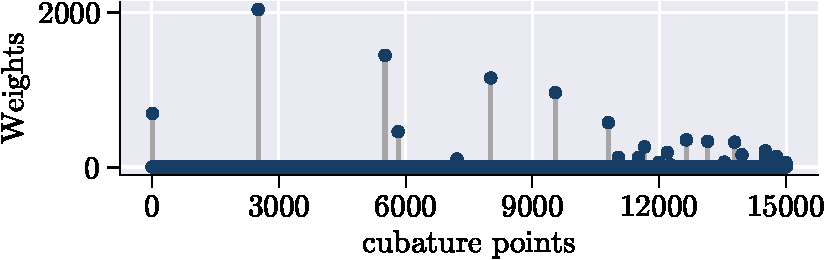
\includegraphics[width=0.8\linewidth]{reduced_mesh_empCM.pdf}
    \caption{Sparse distribution of cubature points and corresponding weights achieved using the ECM-based hyper-reduction technique. The ECM algorithm selected 30 points out of 15,000 cubature points (3 cubature points/element) employed in the high-fidelity model. The resulting reduced mesh effectively contains 26 elements out of 5,000 in the high-fidelity model, accounting for approximately 0.52\% of the total elements in the original mesh.}
    \label{fig:reduced_mesh_ecm}
\end{figure}

\begin{figure}[t!]
\centering
\begin{subfigure}[b]{0.33\linewidth}
\centering
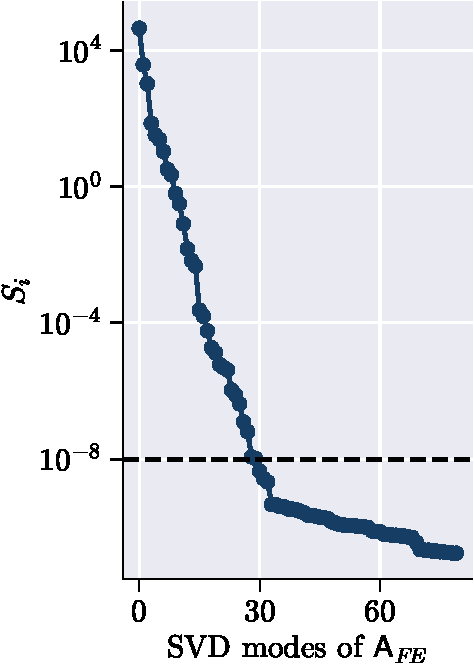
\includegraphics[height=1.3\linewidth]{S_AFE.pdf}
\caption{}
\label{fig:svd_AE}
\end{subfigure}\hfill
\begin{subfigure}[b]{0.33\linewidth}
\centering
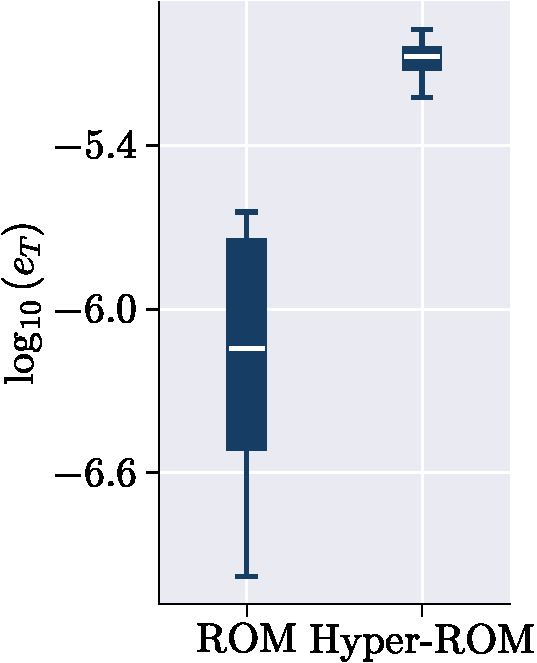
\includegraphics[height=1.3\linewidth]{error_comp_rom_hrom_ecm.pdf}
\caption{}
\label{fig:HROM_ERROR_SPDUP__ecm_a}
\end{subfigure}
\begin{subfigure}[b]{0.33\linewidth}
\centering
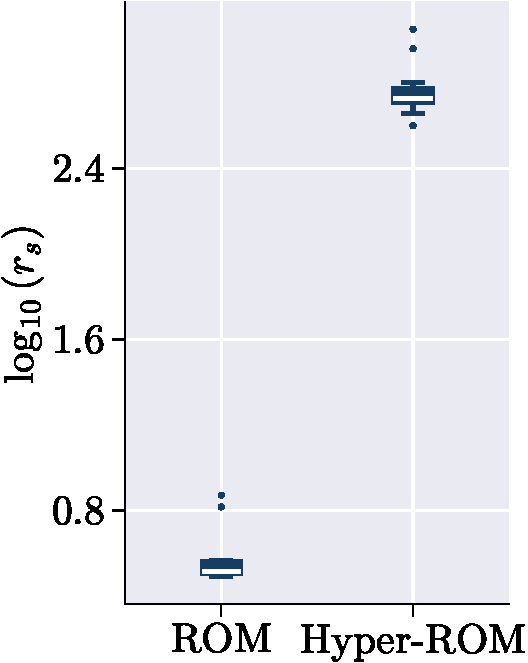
\includegraphics[height=1.3\linewidth]{speed_up_comp_rom_hrom_ecm.pdf}
\caption{}
\label{fig:HROM_ERROR_SPDUP__ecm_b}
\end{subfigure}
\caption{(a) Decay of the singular values of the ECM matrix \(\mat{A}_{FE}\), which is compressed to enhance computational efficiency in identifying a sparse set of cubature points. (b) Difference in accuracy (\(e_T\)) and (c) speed-up (\(r_s\)) between the regular projection-based ROM and the ECM Hyper-ROM.}
\label{fig:HROM_ERROR_SPDUP_ecm}
\end{figure}




\subsection{Deep-learning-based strategies}

In recent years, deep-learning-assisted hyper-reduced ROMs have seen significant advancements \cite{cicci2022deep-hyromneta,romor2025explicable}.
This section offers a concise overview of a few of such strategies.

Deep-learning-based approaches are especially relevant for Nonlinear Manifold ROMs (NM-ROMs) \cite{kim2022fast,jain2017quadratic}.
An NM-ROM represents the solution on a nonlinear manifold $\mathcal{S} := \{\mathscr{G} (\vec{v}) \mid \vec{v} \in \mathbb{R}^{n}\}$, where $\mathscr{G} : \mathbb{R}^{n} \rightarrow \mathbb{R}^{N}$ is a nonlinear function mapping a latent space of dimension $n$ (with $n \ll N$) to the full-order model space of dimension $N$.
The NM-ROM approximates the PDE solution within a trial manifold as follows:
\begin{equation}
    \vec{w}(t,\mu)_N \approx \widetilde{\vec{w}}(t,\mu)_N = \vec{w}^{\text{ref}}_N + \mathscr{G}_n(\vec{w}(t,\mu)),
    \label{eq:NM_ROM_gov}
\end{equation}
where $\vec{w}_n \in \mathbb{R}^{n}$ denotes the reduced coordinates.
The associated time derivative is given by
\begin{equation}
\dot{\vec{w}}_N \approx \dot{\widetilde{\vec{w}}}_N = \mat{J}_g(\vec{w}_n) \dot{\vec{w}}_n,
\end{equation}
where $\mat{J}_g$ denotes the Jacobian of $\mathscr{G}_n$, with the initial condition $\vec{w}_{n}(0,\mu) = \mathscr{H} (\vec{w}_{N}(0,\mu) - \vec{w}_N^{\text{ref}})$, where the nonlinear function  $\mathscr{H} \approx \mathscr{G}^{-1}$ satisfies the following:
\begin{equation}
    \widetilde{\vec{w}}_N - \vec{w}^{\text{ref}}_N \approx \mathscr{G}(\mathscr{H}(\vec{w}_N - \vec{w}^{\text{ref}}_N)).
\end{equation}

So far, we have introduced $\mathscr{G}$ and $\mathscr{H}$ in an abstract sense.
However, identifying \(\mathscr{G}\) and \(\mathscr{H}\) can be challenging; therefore, neural networks, particularly autoencoders, are frequently employed to approximate these functions \cite{kim2022fast}.
Specifically, the decoder serves as \(\mathscr{G}\), while the encoder serves as \(\mathscr{H}\).


The NM-ROM framework deals with two layers of nonlinearities: the nonlinearity in the original governing equations and the nonlinearity of the decoder, which influences the residual of the PDE.
The first layer can be addressed using the hyper-reduction strategies discussed earlier; however, the second layer necessitates special treatment.
The Jacobian of the decoder must be computed at each solver iteration, and its computational cost scales with the number of learnable parameters, potentially reducing computational efficiency.
To mitigate this, a subnet mask can be constructed to compute only the necessary outputs, bypassing the need for the full decoder or its Jacobian.


NM-ROMs are particularly effective for convection-dominated systems described by partial differential equations (PDEs) that exhibit a slow decay of the Kolmogorov $n$-width \cite{lee2020model}.
For such PDEs, the dimension of the linear subspace (\(\widetilde{\mathbb{U}}\)) required to capture the solution is typically characterized by a prohibitively large $n$, diminishing the effectiveness of pROMs and hyper-reduced ROMs.
By leveraging a nonlinear manifold, NM-ROMs directly address this width problem, providing a more efficient solution.


In a parallel effort to overcome the same $n$-width problem, Barnett et al.
\cite{barnett2023neural-network-augmenteda} introduced a neural-network-augmented strategy, but within the framework of LS-ROMs instead of NM-ROMs.
In their proposed framework, termed PROM-ANN, the PDE solution is retained within a linear subspace derived from the left reduced-order basis of the solution snapshot matrix, while incorporating an artificial neural network (ANN) which acts as a corrector to enhance the approximation:
\begin{equation}
  \vec{w}_N(t; \mu) \approx \widetilde{\mathbf{w}}_N(t; \mu) = \mathbf{w}_N^{\text{ref}} +  \widetilde{\mathbb{U}} \vec{w}_n(t; \mu) + \widetilde{\mathbb{U}}^{c} \mathscr{N}(\vec{w}_n(t; \mu)),
  \label{eq:pROM_idea}
\end{equation}
where \(\widetilde{\mathbb{U}}\) is a rank-\(n\) matrix obtained by truncating the first \(n\) dominant proper orthogonal decomposition (POD) modes of the snapshot matrix, and \(\widetilde{\mathbb{U}}^c\) is a rank-\(n_c\) matrix containing the next \(n_c\) POD modes.
The sum of \(n\) and \(n_c\) is chosen to be less than or equal to the rank of the snapshot matrix.
Note that \(\widetilde{\mathbb{U}}^\top \widetilde{\mathbb{U}} = \mat{I}_n\), \(\widetilde{\mathbb{U}}^{c\top} \widetilde{\mathbb{U}}^{c} = \mat{I}_{n_c}\), and \(\widetilde{\mathbb{U}}^\top \widetilde{\mathbb{U}}^c = \mat{0}\).
Here, the value of \(n\) is deliberately chosen to be small to maintain a low-dimensional ROM, implying that \(\widetilde{\mathbb{U}}\) captures a smaller fraction of the snapshot data variance compared to conventional approaches (e.g., 0.9999).



Given a training snapshot \(\vec{w}_N(t_i,\boldsymbol{\mu}_j)\), it can be shown that ideally
\begin{equation}
\label{eq:ann_prom}
\widetilde{\mathbb{U}}^{c\top} (\vec{w}(t_i,\boldsymbol{\mu}_j)_N-\mathbf{w}_N^{\text{ref}}) = \mathcal{N}(\vec{w}_n(t; \mu)) = \vec{w}^c_n
\end{equation}
Even though the equality in \cref{eq:ann_prom} is difficult to achieve in practice,
the neural network \(\mathcal{N}\) can be trained for all solution snapshots in the snapshot matrix, enabling it to output a vector that closely resembles \(\vec{w}^c_n \in \mathbb{R}^{n_c \times 1}\) for a given \(\vec{w}_n\).
Once trained, it is then sufficient to compute \(\vec{w}_n\) using an \(n\)-dimensional ROM and subsequently determine \(\widetilde{\vec{w}}_N\) via \cref{eq:pROM_idea}.
The authors further extended this formulation to develop ECSW-based hyper-reduced LSPG pROMs \cite{barnett2023neural-network-augmenteda}.



\section{Discussion and outlook}
Hyper-reduction methods have emerged as a powerful tool in addressing the computational challenges associated with large-scale nonlinear simulations across various engineering disciplines.
These methods, by efficiently handling nonlinear terms, significantly enhance the computational efficiency of ROMs, making them indispensable for real-time decision-making and large-scale data analysis.
The applications of hyper-reduction techniques span advanced manufacturing, thermal system simulations, reservoir simulations, fluid mechanics, nuclear engineering, structural dynamics, among others, demonstrating their effectiveness in tackling complex simulation challenges.

The development of deep-learning-based hyper-reduction approaches offers promising avenues for further enhancing computational efficiency.
These approaches, which utilize neural networks, can be particularly effective for NM-ROMs.
NM-ROMs represent the solution on a nonlinear manifold, which can be challenging to identify; therefore, neural networks, particularly autoencoders, are frequently employed to approximate these functions.
The use of subnet masks can also mitigate the computational cost associated with computing the Jacobian of the decoder, enhancing the efficiency of NM-ROMs.

The integration of hyper-reduction methods into commercial software tools is crucial for realizing their full potential in various engineering applications.
However, the lack of hyper-reduction capabilities in commercial software, as illustrated in Figure 3, presents a missed opportunity for commercial platforms.
This gap is primarily due to the intrusive nature of these techniques, which requires extensive modifications to existing codebases and databases within well-established computational pipelines.
Open-source tools, on the other hand, tend to have more flexibility to integrate such methods, but commercial platforms prioritize stability and broad applicability, making it challenging to adopt hyper-reduction without causing significant disruptions.

Despite these challenges, the potential benefits of hyper-reduction methods are substantial, particularly the integration of hyper-reduction techniques into digital twins presents a transformative potential for enhancing computational efficiency and real-time interaction capabilities.
The use of hyper-reduction methods can significantly optimize these processes, making digital twins more effective and responsive.
\begin{itemize}
\item \textit{Enhancing Computational Efficiency}

Hyper-reduction streamlines computational processes by reducing the complexity of models while maintaining essential features and accuracy. This reduction is crucial for digital twins, which often need to process vast amounts of data quickly to simulate real-world conditions effectively. By employing hyper-reduction, digital twins can handle nonlinearities more efficiently, allowing them to perform complex simulations without excessive computational overhead.

\item \textit{Real-Time Interaction and Decision-Making}

The ability of digital twins to interact with their physical counterparts in real-time is invaluable in many real-world applications. Hyper-reduction techniques facilitate this interaction by enabling faster processing speeds and reducing latency in data analysis and model updates. This capability ensures that digital twins can provide timely insights and support rapid decision-making processes, optimizing performance across various applications.

\item \textit{Optimizing Performance and Reducing Downtime}

With hyper-reduction methods, digital twins can help reduce downtime and improve operational efficiency. For instance, in industrial settings, digital twins enhanced with hyper-reduction techniques can simulate different scenarios to predict equipment failures or maintenance needs, thereby minimizing disruptions and extending the lifespan of machinery.

\item \textit{Facilitating Predictive Maintenance}

By continuously analyzing real-time data from sensors and other inputs, these digital twins can forecast when maintenance should be performed to prevent failures. This predictive capability not only saves costs associated with unscheduled downtime but also enhances the reliability and safety of operations.

\item \textit{Enhance Verification, Validation, and Uncertainty Quantification (VVUQ) of Digital Twins}

VVUQ plays an important role in all elements of the digital twin ecosystem \cite{engineering2024foundational}. Hyper-reduction methods can help enhance VVUQ processes in digital twins by increasing computational efficiency, improving model fidelity, and enabling real-time data integration. These improvements ensure that digital twins remain accurate and reliable tools for simulation and decision-making across various industries.

\end{itemize}

In conclusion, hyper-reduction methods hold significant potential for advancing computational efficiency across various disciplines.
Their integration into commercial software and further development through deep-learning-based approaches will be crucial for realizing their full potential in various applications.
By efficiently handling nonlinearities, hyper-reduction methods can facilitate the effective deployment of digital twins, optimize performance, reduce downtime, and facilitate real-time interaction between the physical and virtual worlds.


\bibliographystyle{unsrtnat}
\bibliography{reference_v5.bib}
\appendix








        


    










    
    
    
    































































\section{Key Jargons}
\label{sec:glossary}



\begin{itemize}
    \item \textbf{Subspace:} A subspace is a subset of a vector space that is itself a vector space under the same operations. A subspace must contain the zero vector, be closed under addition, and be closed under scalar multiplication.

    \item \textbf{Affine Subspace:} An affine subspace is a subset of a vector space that is closed under affine combinations. It can be viewed as a linear subspace that has been translated from the origin.

    \item \textbf{Manifold:} A manifold is a mathematical space that locally resembles Euclidean space near each point. Manifolds are used to generalize concepts such as curves and surfaces to higher dimensions.

    \item \textbf{Latent Space:} A latent space is a lower-dimensional space that captures the essential features of the data. For example, subspace spanned by the dominant POD modes. In a neural network setting, encoders map data to this space, and decoders reconstruct the data from it.

    \item \textbf{Modal Energies (SVD):} In singular value decomposition (SVD), modal \textit{energies} refer to the singular values, which represent the amount of \textbf{variance} captured by each mode in the data. The term \textit{energy} is essentially a misnomer, which often as nothing to do with the physical energy of the system \cite{bhattacharyya2020energy}.

    \item \textbf{Offline and Online:} In model reduction, ``offline'' refers to computations done prior to real-time use, often involving expensive and time-consuming tasks. ``Online'' refers to computations done in real-time, typically leveraging precomputed data to achieve fast and efficient results.

    \item \textbf{Residual:} The residual is the difference between the left and right sides of a differential equation after substituting an approximate solution. It provides a measure of how well the approximate solution satisfies the original equation.

    \item \textbf{Snapshots:} In model reduction, snapshots are sample solutions of the full-order model used to construct a reduced-order basis. These solutions are typically obtained by solving the original problem for different parameter values and/or at different time instants.

    \item \textbf{Affine Decomposition:} Affine decomposition is a mathematical technique commonly used in reduced order modeling (ROM), particularly for parametric problems. It separates the parametric dependencies in equations, enabling efficient computations for a wide range of parameter values.

    \textbf{Parametric Separation}:
    
       - A parametric problem is expressed in a form where the parameter dependency is isolated.
       
       - For example, consider a linear problem:
         \[
         A(\boldsymbol{\mu}) \mathbf{u} = \mathbf{f}(\boldsymbol{\mu}),
         \]
         where \(\boldsymbol{\mu}\) is a vector of parameters. Using affine decomposition, \(A(\boldsymbol{\mu})\) and \(\mathbf{f}(\boldsymbol{\mu})\) are represented as:
         \[
         A(\boldsymbol{\mu}) = \sum_{q=1}^Q \Theta_q^A(\boldsymbol{\mu}) A_q,
         \]
         \[
         \mathbf{f}(\boldsymbol{\mu}) = \sum_{q=1}^Q \Theta_q^f(\boldsymbol{\mu}) \mathbf{f}_q.
         \]
    
    \textbf{Offline-Online Decoupling}:
    
       - \textit{Offline Phase}: Parameter-independent terms (\(A_q\) and \(\mathbf{f}_q\)) are precomputed and stored.
       
       - \textit{Online Phase}: For a new parameter \(\boldsymbol{\mu}\), the computational effort involves only evaluating the parameter-dependent functions (\(\Theta_q^A(\boldsymbol{\mu})\) and \(\Theta_q^f(\boldsymbol{\mu})\)) and combining the precomputed terms.
    
    \item \textbf{Galerkin Projection:} Galerkin projection is a method for solving differential equations by projecting the infinite-dimensional problem onto a finite-dimensional subspace. Let \( V \) be the space in which the solution resides, and \( V_r \) be the finite-dimensional subspace (spanned by basis functions \( \{ \boldsymbol\phi_1, \boldsymbol\phi_2, \ldots, \boldsymbol\phi_r \} \)). The Galerkin projection seeks an approximate solution \( u_r \) in \( V_r \) such that the residual \( R(u_r) \) is orthogonal to the subspace \( V_r \):
    \[
    \text{Find } u_r \in V_r \text{ such that } \left( R(u_r), \phi_i \right) = 0, \quad \forall \, i = 1, 2, \ldots, r
    \]
    where \( R(u_r) \) is the residual, and \( \left( \cdot, \cdot \right) \) denotes the inner product.

    \item \textbf{Petrov-Galerkin Projection:} Petrov-Galerkin projection is a generalization of the Galerkin method, where the trial and test spaces are different. Given a trial space \( V_r \) and a test space \( W_r \), the Petrov-Galerkin method finds an approximate solution \( u_r \) in \( V_r \) such that the residual \( R(u_r) \) is orthogonal to the test space \( W_r \):
    \[
    \text{Find } u_r \in V_r \text{ such that } \left( R(u_r), \psi_i \right) = 0, \quad \forall \, i = 1, 2, \ldots, r
    \]
    where \( \psi_i \) are the basis functions of the test space \( W_r \). This approach is often used to improve stability and accuracy, especially in non-symmetric or convection-dominated problems.

    \begin{figure}[t]
    \centering
    \begin{subfigure}[b]{0.35\linewidth}
    \centering
    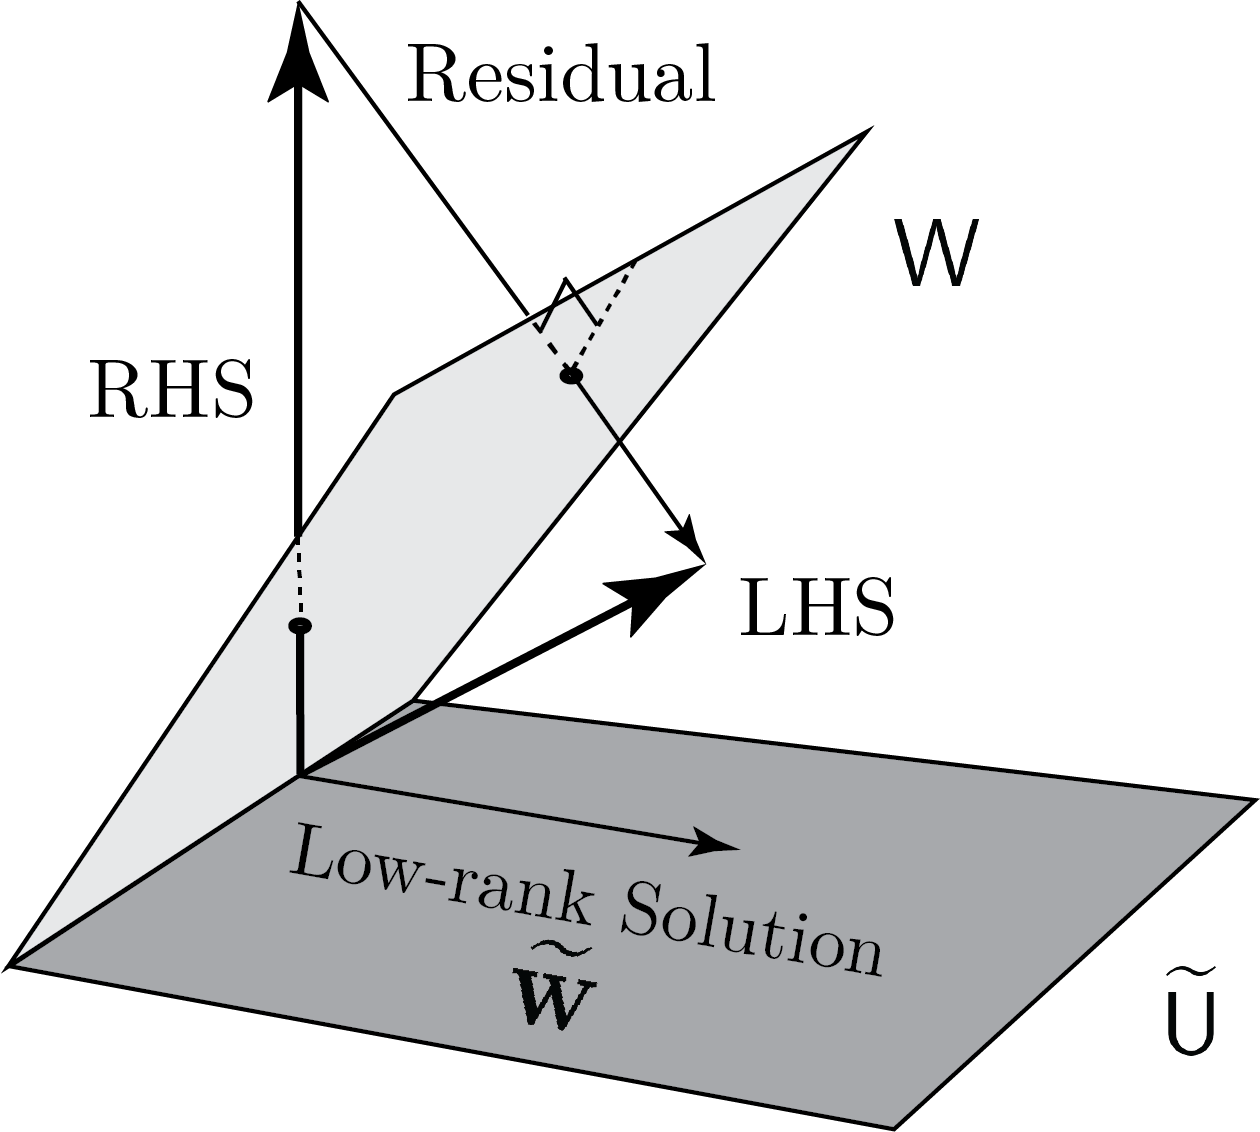
\includegraphics[width=\linewidth]{PG.png}
    \caption{}
    \label{fig:projections_PG}
    \end{subfigure}\hfill
    \begin{subfigure}[b]{0.35\linewidth}
    \centering
    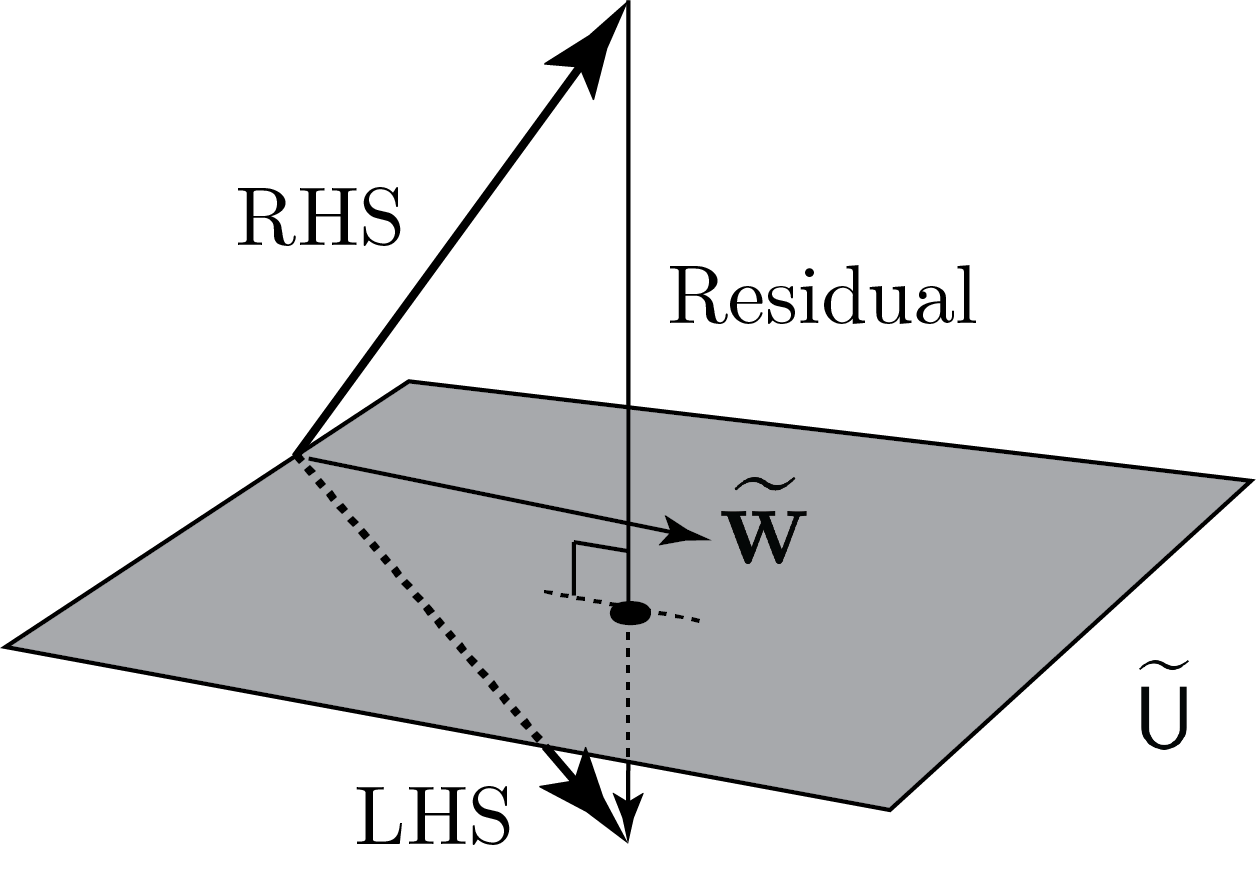
\includegraphics[width=\linewidth]{G.png}
    \caption{}
    \label{fig:projections_G}
    \end{subfigure}
    \caption{(a) Petrov-Galerkin Projection (b) Galerkin Projection}
    \label{fig:projections}
    \end{figure}

    \item \textbf{Left ROB and Right ROB:} Reduced-order bases (ROB) are used in model reduction techniques. The left ROB is associated with the solution space, ${\mathbb{U}}$, while the right ROB, ${\mathbb{W}}$ is typically associated with the test space (in Petrov-Galerkin projection).

    \item \textbf{Weak Form:} The weak form of a partial differential equation is obtained by multiplying the equation by a test function \( v \) and integrating over the domain, often leading to a variational problem. For a PDE \( \mathcal{L}(u) = f \) on \( \Omega \), the weak form is:
    \[
    \text{Find } u \in V \text{ such that } \int_\Omega \mathcal{L}(u) v \, d\Omega = \int_\Omega f v \, d\Omega \quad \forall \, v \in V
    \]
    where \( V \) is an appropriate function space. The weak form is fundamental in the finite element method as it allows for more flexible function spaces.

    \item \textbf{Oblique Projection Matrix}: An oblique projection matrix is a linear transformation matrix \( P \) that projects vectors onto a subspace \( M \) along a direction that is not necessarily perpendicular to \( M \). Given matrices \( \mat{A} \) and \( \mat{B} \):
    \[
    \mat{P} = \mat{A} (\mat{B}^\top \mat{A})^{-1} \mat{B}^\top
    \]
    provided \( \mat{B}^\top \mat{A} \) is invertible.
\end{itemize}

\section{Algorithms}
\label{sec:algorithms}







            
            
            
            



\subsection{Empirical Interpolation Method (EIM)}
Given a \textit{continuous} nonlinear function $f: \overline{\Omega} \times \mathcal{P}_{\text{EIM}} \rightarrow \mathbb{R}$, where $\overline{\Omega}$ is the spatial domain and $\mathcal{P}_{\text{EIM}}$ is the parameter space, EIM aims to approximate $f$ using a finite sum of basis functions $\{ U_q \}_{q=1}^Q$ evaluated at specific interpolation points $\{ x_q \}_{q=1}^Q$:
\[
f(x, w^\mu;\mu) \approx \sum_{q=1}^Q c_q(\mu) U_q(x),
\]
where the coefficients $c_q(\mu)$ are determined by enforcing the interpolation conditions:
\[
f(x_i, w^\mu;  \mu) = \sum_{q=1}^Q c_q(\mu) U_q(x_i), \quad \text{for } i = 1, \ldots, Q.
\]
This approach reduces the problem of evaluating \( f \) over the entire domain \( \Omega \) to computing it at a finite number of points \( \{ x_q \} \), thus enhancing computational efficiency.


\begin{algorithm}
\caption{EIM Algorithm for Nonlinear Term Approximation}
\begin{algorithmic}[1]
\STATE \textbf{Input:}$f$, $\overline{\Omega}$, $\mathcal{P}_{\text{EIM}}$, $tol$
\STATE \textbf{Output}: Basis functions $\{ U_q \}_{q=1}^Q$, Interpolation points $\{ x_q \}_{q=1}^Q$
\STATE \textcolor{blue}{Initialization:}
\STATE \textbf{Set:} iteration counter $q = 1$
\STATE \textbf{Initialize:} the interpolation operator $\mathcal{I}_0[f] = 0$
\STATE \textbf{Collect:} snapshots $[f(x, w^{\mu_1}; \mu_1), \ldots, f(x, w^{\mu_Q}; \mu_Q)]$ evaluated at selected parameters
\WHILE{$err_q > tol$ AND $q \le Q$}
    \STATE $ \mu_q = \arg \max_{\mu \in \mathcal{P}_{\text{EIM}}} \left\| f(\cdot, w^\mu; \mu) - \mathcal{I}_{q-1}[ f(\cdot, w^\mu; \mu) ] \right\|_{L^\infty(\Omega)} $ \textcolor{blue}{// Selection of Parameter}\vspace{6pt}
    \STATE $ x_q = \arg \max_{x \in \Omega} \left| f(x, w^{\mu_q}; \mu_q) - \mathcal{I}_{q-1}[ f(x, w^{\mu_q}; \mu_q) ] \right| $ \textcolor{blue}{// Selection of Interpolation Point:}\vspace{6pt}
    \STATE $ U_q(x) = \dfrac{ f(x, w^{\mu_q}; \mu_q) - \mathcal{I}_{q-1}[ f(x, w^{\mu_q}; \mu_q) ] }{ f(x_q, w^{\mu_q}; \mu_q) - \mathcal{I}_{q-1}[ f(x_q, w^{\mu_q}; \mu_q) ] } $ \textcolor{blue}{// Construction of Basis Function:}\vspace{6pt}
    \STATE $T_{ij} = U_j(x_i)$ satisfying $T_{ii} = 1$ and $T_{ij} = 0$ for $1 \leq i < j$ \textcolor{blue}{// Properties of Interpolation Matrix:}\vspace{6pt}
    \STATE $   \mathcal{I}_q[ f(x, w^{\mu}; \mu) ] = \sum_{j=1}^q c_j(\mu) U_j(x) $ \textcolor{blue}{// Update of Interpolation Operator, where $\vec{c}(\mu)$ is solved using the linear system $\mat{T} \vec{c}(\mu) = \vec{f}(\mu)$}\vspace{6pt}
    \STATE $ err_q = \sup_{\mu \in \mathcal{P}_{\text{EIM}}} \left\| f(\cdot, w^\mu; \mu) - \mathcal{I}_q[ f(\cdot, w^\mu; \mu) ] \right\|_{L^\infty(\Omega)}$  \textcolor{blue}{// check error}\vspace{6pt}
    \IF{$err_q > tol$}
        \STATE increment $q = q + 1$
    \ELSE
        \STATE exit loop
    \ENDIF
\ENDWHILE
\end{algorithmic}
\end{algorithm}
\subsection{S-OPT Sampling Algorithm}
\begin{algorithm}[H]
\caption{S-OPT Sampling Algorithm (Adapted from \cite{lauzon2024s-opt}).}
\begin{algorithmic}[1]
\STATE \textbf{Input:} Basis matrix $\mathsf{F}_{\text{basis}}$ of shape $(n_{\text{rows}}, n_f)$
\STATE \textbf{QR Factorization} - Obtain orthogonal basis $\mathsf{Q}$ from $\mathsf{F}_{\text{basis}}$ \textcolor{blue}{// Perform QR factorization on the input basis}
\STATE $\mathsf{Q}, \_ = \text{qr}(\mathsf{F}_{\text{basis}})$ \textcolor{blue}{// $\mathsf{Q}$ is an orthogonal matrix representing the basis}
\STATE \textbf{Initialize} $\mathcal{Z} = \{i^*\}$ where $i^* = \arg\max_i |\mathsf{Q}_{i,1}|$ \textcolor{blue}{// Select the index with the largest measure of $S$}
\FOR{$j = 1$ \textbf{to} $n_f - 1$}
    \STATE Construct $\mathsf{Z} = [\mathit{e}_i]_{i \in \mathcal{Z}}$, $\mathsf{A} = \mathsf{Z}^\top \mathsf{Q} [\mathsf{E}_1, \cdots, \mathsf{E}_j]$, $\mathbf{c} = \mathsf{Z}^\top \mathsf{Q} \mathit{e}_{j+1}$, and $\mathbf{g} = (\mathsf{A}^\top \mathsf{A})^{-1} \mathsf{A}^\top \mathbf{c}$ \textcolor{blue}{// Construct necessary components, where $\mathit{e} \in \mathbb{R}^{n_{\text{rows}}}$ and $\mathsf{E} \in \mathbb{R}^{n_{f\text{rows}} \times 1}$}
    \STATE Find $i^* = \arg\max_{i \notin \mathcal{Z}} \dfrac{1 + \mathbf{r}^\top \mathbf{b}}{\prod_{k=1}^{j} (\|\mathsf{Ae_k}\|^2 + r_k^2)} \dfrac{\mathbf{c}^\top \mathbf{c} + \gamma^2 - \alpha}{\mathbf{c}^\top \mathbf{c} + \gamma^2}$ \textcolor{blue}{// Identify the index with the optimal value}
    \STATE where $\mathbf{r}^\top = \mathit{e}_i^\top \mathsf{Q} [\mathsf{E}_1, \cdots, \mathsf{E}_j]$, $\mathbf{b} = (\mathsf{A}^\top \mathsf{A})^{-1} \mathbf{r}$, $\gamma = \mathsf{Q}_{i,j+1}$, \newline$\alpha = (\mathbf{c}^\top \mathsf{A} + \gamma \mathbf{r}^\top) \left( \mathsf{I} - \dfrac{\mathbf{b} \mathbf{r}^\top}{1 + \mathbf{r}^\top \mathbf{b}} \right) (\mathbf{g} + \gamma \mathbf{b})$ \textcolor{blue}{// Calculate necessary components for optimization}
    \STATE Enrich $\mathcal{Z} \leftarrow \mathcal{Z} \cup \{i^*\}$ \textcolor{blue}{// Add the new index to the sampling set}
\ENDFOR
\STATE \textbf{Output} $\mathcal{Z}$
\textcolor{blue}{// Oversampling Procedure}
\STATE \textbf{Initialize} $\mathcal{Z} = \{i^*\}$ where $i^* = \arg\max_i |\mathsf{Q}_{i,1}|$ \textcolor{blue}{// Select the index with the largest measure of $S$}
\FOR{$j = 1$ \textbf{to} $n_f - 1$}
    \STATE Construct $\mathsf{Z} = [\mathit{e}_i]_{i \in \mathcal{Z}}$ and $\mathsf{A} = \mathsf{Z}^\top \mathsf{Q}$ \textcolor{blue}{// Construct the current basis matrix, where $\mathit{e} \in \mathbb{R}^{n_{\text{rows}}}$}
    \STATE Find $i^* = \arg\max_{i \notin \mathcal{Z}} \dfrac{1 + \mathbf{r}^\top (\mathsf{A}^\top \mathsf{A})^{-1} \mathbf{r}}{\prod_{k=1}^{n_f} (\|\mathsf{Ae_k}\|^2 + r_k^2)}$ with $\mathbf{r}^\top = \mathit{e}_i^\top \mathsf{Q}$ \textcolor{blue}{// Select index based on the oversampling criterion}
    \STATE Enrich $\mathcal{Z} \leftarrow \mathcal{Z} \cup \{i^*\}$ \textcolor{blue}{// Add the new index to the sampling set}
\ENDFOR
\STATE \textbf{Output} $\mathcal{Z}$
\end{algorithmic}
\label{alg:S_OPT}
\end{algorithm}









\subsection{Point Selection in Empirical Cubature Method (ECM)}
\begin{algorithm}[H]
\caption{Empirical Cubature Method (Reproduced from \cite{bravo2024subspace})}
\label{alg:ECM_PS}
\begin{algorithmic}[1]
\STATE \textbf{Function} $[ \varepsilon, \boldsymbol\omega] = \text{ECM}(\widetilde{\mathbb{W}}, \vec{W}_{FE}, y^0)$
\STATE \textbf{Data}: $\widetilde{\mathbb{W}} \in \mathbb{R}^{K \times M}$, where $\widetilde{\mathbb{W}}^\top \widetilde{\mathbb{W}} = I$; $\vec{W}_{FE} \in \mathbb{R}^{M\times 1}$; $y^0 \subset \{1, 2, ..., M\}$: initial candidates; $\lambda \leftarrow 10$, threshold number of ineffective iterations
\STATE \textbf{Result}: $\varepsilon \subset \{1, 2, ..., M\}$; $\boldsymbol\omega > 0$ such that $ \widetilde{\mathbb{W}}(\varepsilon, :)^\top \boldsymbol\omega = \widetilde{\mathbb{W}}^\top \vec{W}_{FE}$ and $\text{card}(\varepsilon \cap y^0)$ is maximum.
\algstore{myalg2}
\end{algorithmic}
\end{algorithm}
\begin{algorithm}[H]                  
\begin{algorithmic} [1]                   %
\algrestore{myalg2}
\IF{$y^0 = \emptyset$ \textcolor{blue}{// no initial candidate set given}} 
    \STATE $y\leftarrow \{1, 2, ..., M\}$
    \STATE $y\leftarrow \{h_1, h_2, \dots\}$ such that $\| \widetilde{\mathbb{W}}(h_i, :) \| \leq \varepsilon$ \textcolor{blue}{// Remove low norm points on the candidate set ($\sim 10^{-10}$)}
\ELSE
    \STATE $y' \leftarrow \{1, 2, ..., M\} \setminus y^0$; \quad $y\leftarrow y^0$
    \STATE $y' \leftarrow \{h_1, h_2, \dots\}$ such that $\| \widetilde{\mathbb{W}}(h_i, :) \| \leq \varepsilon$ \textcolor{blue}{// Remove low norm points on the complement set ($\sim 10^{-10}$)}
\ENDIF
\STATE $\varepsilon \leftarrow \emptyset$; $\vec{b} \leftarrow \widetilde{\mathbb{W}}^\top \vec{W}_{FE}$; $\vec{r} \leftarrow \vec{b}$; $\boldsymbol\omega \leftarrow \emptyset$; $H \leftarrow \emptyset$ \textcolor{blue}{// Initializations}
\STATE $\phi \leftarrow 0$ \textcolor{blue}{// Failed iterations counter}

\WHILE{$\text{length}(\varepsilon) < p$ \textbf{AND} $\text{length}(y) > 0$}
    \IF{$\phi > \lambda$}
        \STATE $y\leftarrow y \cup y'$ \textcolor{blue}{// Enlarge candidate set to include the complement set}
    \ENDIF

    \STATE $j = \arg\max_{j \in y} \vec{g}_j^\top \vec{r}$, where $\vec{g}_j = \widetilde{\mathbb{W}}(j, :) / \| \widetilde{\mathbb{W}}(j, :) \|$ \textcolor{blue}{// Select the row most "positively" parallel to the residual}

    \IF{$\varepsilon = 0$}
        \STATE $\mat{H}\leftarrow (\widetilde{\mathbb{W}}(i, :) \widetilde{\mathbb{W}}(i, :)^\top)^{-1}$ \textcolor{blue}{// Inverse Hermitian matrix (first iteration)}
        \STATE $\boldsymbol\omega \leftarrow \mat{H}\widetilde{\mathbb{W}}(i, :)^\top \vec{b}$ \textcolor{blue}{// Weights computed through least-squares}
    \ELSE
        \STATE $[\boldsymbol\omega, \mat{H}] \leftarrow \text{LSTQNER}(i, \mat{H}, \widetilde{\mathbb{W}}(\varepsilon, :), \widetilde{\mathbb{W}}(i, :), \vec{r}, \vec{b})$ \textcolor{blue}{// Least-squares via rank-one update, see Algorithm 8 in Ref.~\cite{bravo2024subspace}}
    \ENDIF

    \STATE $\varepsilon \leftarrow \varepsilon \cup i$; $y\leftarrow y \setminus \{i\}$ \textcolor{blue}{// Move index $i$ from $y$ to $\varepsilon$}
    \STATE $n \leftarrow$ Indexes such that $\boldsymbol\omega(n) < 0$ \textcolor{blue}{// Identify negative weights}
    \STATE $y\leftarrow y \cup \{\varepsilon(n)\}$; $\varepsilon \leftarrow \varepsilon \setminus \{\varepsilon(n)\}$ \textcolor{blue}{// Remove indexes with negative weights}
    \STATE $\mat{H}\leftarrow \text{UPHERM}(\mat{H}, n)$ \textcolor{blue}{// Update inverse Hermitian Matrix (see Algorithm 9 in Ref.~\cite{bravo2024subspace})}
    \STATE $\boldsymbol\omega \leftarrow \mat{H}\widetilde{\mathbb{W}}(\varepsilon, :)^\top \vec{b}$ \textcolor{blue}{// Recalculate weights}
    \IF{successful iteration}
        \STATE $\phi \leftarrow 0$
    \ELSE
        \STATE $\phi \leftarrow \phi + 1$
    \ENDIF

    \STATE $\vec{r} \leftarrow \vec{b} - \widetilde{\mathbb{W}}(\varepsilon, :)^\top \boldsymbol\omega$ \textcolor{blue}{// Update the residual}
\ENDWHILE
\end{algorithmic}
\end{algorithm}


\subsection{Point Selection in GNAT hyper-reduction}
\begin{algorithm}[H]
\caption{Greedy algorithm for selecting sample nodes from a given  mesh (reproduced from \cite{carlberg2013gnat})}
\label{greedy}
\begin{algorithmic}[1]
\REQUIRE {$\widetilde{\mathbb{U}}_R$ (POD basis for residuals), $\widetilde{\mathbb{U}}_J$ (POD basis for Jacobians), target sample nodes $m_{\mathrm{node}}$, initial sample-node set $\mathcal{N}$ (see Remark 2), and number of working columns $n_c \leq \min(m_R, m_J, \nu m_{\mathrm{node}})$, where $\nu$ denotes the number of unknowns at a node (e.g., $\nu = 5$ for three-dimensional compressible flows without a turbulence model).}
\ENSURE{sample-node set $\mathcal{N}$}
\STATE Compute the additional number of nodes to sample: $n_a = m_{\mathrm{node}} - |\mathcal{N}|$
\STATE Initialize counter for the number of working basis vectors used: $n_b \leftarrow 0$
\STATE Set the number of greedy iterations to perform: $n_{\mathrm{it}} = \min(n_c, n_a)$ 
\STATE Compute the maximum number of right-hand sides in the least-squares problems: $n_{\mathrm{RHS}} = \mathrm{ceil}(n_c / n_a)$
\STATE Compute the minimum number of working basis vectors per iteration: $n_{ci,\mathrm{min}} = \mathrm{floor}(n_c / n_{\mathrm{it}})$
\STATE Compute the minimum number of sample nodes to add per iteration: $n_{ai,\mathrm{min}} = \mathrm{floor}(n_a n_{\mathrm{RHS}} / n_c)$
\FOR[greedy iteration loop]{$i = 1, \ldots, n_{\mathrm{it}}$}
\STATE Compute the number of working basis vectors for this iteration: $n_{ci} \leftarrow n_{ci,\mathrm{min}}$; 
\\ if ($i \leq n_c \mod n_{\mathrm{it}}$), then $n_{ci} \leftarrow n_{ci} + 1$
\STATE Compute the number of sample nodes to add during this iteration: $n_{ai} \leftarrow n_{ai,\mathrm{min}}$; 
\\ if ($n_{\mathrm{RHS}} = 1$) and ($i \leq n_a \mod n_c$), then $n_{ai} \leftarrow n_{ai} + 1$
\IF{$i = 1$}
\STATE $[\vec{r}^1 \ldots \vec{r}^{n_c}] \gets [\widetilde{\mathbb{U}}_R^1 \ldots \widetilde{\mathbb{U}}_R^{n_c}]$
\STATE $[\mathsf{J}^1 \ldots \mathsf{J}^{n_c}] \gets [\widetilde{\mathbb{U}}_J^1 \ldots \widetilde{\mathbb{U}}_J^{n_c}]$
\ELSE
\FOR{$q = 1, \ldots, n_{ci}$} \{basis vector loop\}
\STATE $\vec{r}^q \gets \widetilde{\mathbb{U}}_R^{n_b+q} - [\widetilde{\mathbb{U}}_R^1 \ldots \widetilde{\mathbb{U}}_R^{n_b}] \alpha$, with $\alpha = \arg \min_{\gamma \in \mathbb{R}^{n_b}} \| [Z^\top \widetilde{\mathbb{U}}_R^1 \ldots Z^\top \widetilde{\mathbb{U}}_R^{n_b}] \gamma - Z^\top \widetilde{\mathbb{U}}_R^{n_b+q} \|_2$
\STATE $\mathsf{J}^q \gets \widetilde{\mathbb{U}}_J^{n_b+q} - [\widetilde{\mathbb{U}}_J^1 \ldots \widetilde{\mathbb{U}}_J^{n_b}] \beta$, with $\beta = \arg \min_{\gamma \in \mathbb{R}^{n_b}} \| [Z^\top \widetilde{\mathbb{U}}_J^1 \ldots Z^\top \widetilde{\mathbb{U}}_J^{n_b}] \gamma - Z^\top \widetilde{\mathbb{U}}_J^{n_b+q} \|_2$
\ENDFOR
\ENDIF
\FOR{$j = 1, \ldots, n_{ai}$} \{sample node loop\}
\STATE Choose node with largest average error: $n \gets \arg \max_{l \notin \mathcal{N}} \sum_{q=1}^{n_{ci}} \left( \sum_{i \in \delta(l)} \left((\vec{r}_i^q)^2 + (\mathsf{J}_i^q)^2\right) \right)$,
\STATE where $\delta(l)$ denotes the degrees of freedom associated with node $l$.
\STATE $\mathcal{N} \gets \mathcal{N} \cup \{n\}$
\ENDFOR
\STATE $n_b \gets n_b + n_{ci}$
\ENDFOR
\end{algorithmic}
\end{algorithm}




\end{document}